\documentclass[10pt]{article}

\usepackage[letterpaper,margin=1in]{geometry}
\usepackage[T1]{fontenc}
\usepackage[utf8]{inputenc}
\usepackage{amsmath,amsthm}
\usepackage{newtxtext,newtxmath}
\usepackage{microtype}
\usepackage{mathtools}
\usepackage{booktabs,longtable,tabularx,array,multirow}
\usepackage{graphicx}
\usepackage[font=small,labelfont=bf]{caption}
\usepackage{subcaption}
\usepackage{tikz}
\usepackage{pgfplots}
\pgfplotsset{compat=1.16}
\usepackage{enumitem}
\usepackage{xcolor}
\usepackage{fancyhdr}
\usepackage{hyperref}
\usepackage[nameinlink,noabbrev]{cleveref}

\definecolor{linkblue}{HTML}{164E63}
\hypersetup{
  colorlinks=true,
  linkcolor=linkblue,
  citecolor=linkblue,
  urlcolor=linkblue,
  pdftitle={Extremal Connected Still Lifes in Square Boards},
  pdfauthor={Siddhartha Mahajan}
}
\graphicspath{{figures/}}
\setlist[itemize]{leftmargin=*,nosep}
\setlist[enumerate]{leftmargin=*,nosep}
\renewcommand{\arraystretch}{1.08}
\allowdisplaybreaks

\pagestyle{fancy}
\fancyhf{}
\fancyhead[L]{Extremal Connected Still Lifes}
\fancyhead[R]{Mahajan}
\fancyfoot[C]{\thepage}
\setlength{\headheight}{13.6pt}

\newtheorem{theorem}{Theorem}[section]
\newtheorem{proposition}[theorem]{Proposition}
\newtheorem{lemma}[theorem]{Lemma}
\newtheorem{corollary}[theorem]{Corollary}
\newtheorem{definition}[theorem]{Definition}
\theoremstyle{remark}
\newtheorem{remark}[theorem]{Remark}
\crefname{definition}{definition}{definitions}
\Crefname{definition}{Definition}{Definitions}

\newcommand{\B}{\mathcal B}
\newcommand{\N}{\mathcal N}
\newcommand{\Pop}{\operatorname{pop}}
\newcommand{\Dfour}{D_4}
\newcommand{\Rminus}{\mathcal R_{-2}}
\newcommand{\bits}{\{0,1\}}

\title{\bfseries Extremal Connected Still Lifes in Square Boards}
\author{
Siddhartha Mahajan\\[5pt]
\small Lossfunk Research Laboratory, Bengaluru, Karnataka, India\\[4pt]
\scriptsize Corresponding author: \href{mailto:siddharthamahajan03@gmail.com}{\texttt{siddharthamahajan03@gmail.com}}
}
\date{October 2026}

\begin{document}
\maketitle

\begin{abstract}
Let $C(n)$ denote the largest population of a stable Conway Life pattern in an
$n\times n$ square whose live cells form one component under Moore adjacency;
the exterior of the square is dead.  We determine
\[
\begin{aligned}
C(1),\ldots,C(25)={}&0,4,6,8,11,18,28,32,43,53,63,76,88,\\
&102,119,134,151,170,188,210,230,251,276,299,325
\end{aligned}
\]
and the further values $C(29)=435$, $C(31)=497$, $C(32)=528$,
$C(33)=562$, $C(37)=704$, $C(39)=782$, $C(41)=863$, $C(45)=1037$,
$C(49)=1228$, $C(53)=1434$, $C(57)=1657$, and $C(65)=2150$.  The first
unresolved case satisfies $350\le C(26)\le352$, and every unresolved size
$n\le50$ has a gap of at most five cells.

A live $2\times2$ block is an isolated Moore component, so every connected
still life with more than four cells is block-free.  Combining this local
obstruction with the Chu--Stuckey wastage identity yields finite-state
boundary relaxations, and exact min-plus composition of edge automata and
corner relations gives, for every $n\ge14$,
\[
 C(n)\le \min\!\left\{M(n),
 \left\lfloor\frac{4n^2+5n-d_{n\bmod8}}8\right\rfloor\right\},
 \qquad
 (d_0,\ldots,d_7)=(26,23,18,23,20,23,26,11),
\]
where $M(n)$ is the unrestricted maximum.  Explicit period-eight band
families give $C(n)\ge n(n+1)/2-4$ for every $n\ge1$, with equality of the
constant at $n=5$ and $n=8$, and hence $\lim_{n\to\infty}C(n)/n^2=1/2$.
\end{abstract}

\section{Introduction}

A still life is a fixed point of Conway's Game of Life: each live cell has two
or three live neighbours, and each dead cell has a number of live neighbours
different from three.  In the finite maximum-density problem the live set is
confined to an $n\times n$ square and every cell outside the square is dead.
Exact methods for this problem include variable elimination and boundary
relaxations~\cite{larrosa-2005,chu-stuckey-garcia-2009}, and the unrestricted
optimum, denoted $M(n)$ below, was completely determined by Chu and
Stuckey~\cite{chu-stuckey-2012}.

The connected problem, posed as a benchmark of the 2013 Answer Set Programming
Competition~\cite{drescher-2013}, adds a global condition: the live cells must
form one component under horizontal, vertical, and diagonal adjacency.  This
is not a small perturbation.  Dense unrestricted optima often consist of a
large maze and several stable $2\times2$ blocks, and such a block cannot be
attached to any other live cell, so it is forbidden in every connected pattern
of population greater than four.  The problem was also one of the challenges of
the Verifiable Problems Track of CAISc 2026~\cite{caisc-problem}, posed for the
thirteen sizes $8,9,10,11,13,15,16,17,19,20,21,31,32$.  There, an accepted
artifact is a board checked by a deterministic verifier, that is, a lower
bound.  The seven accepted submissions on this
problem~\cite{caisc-collier,caisc-jaswal,caisc-menta,caisc-reddy,caisc-rushdi,caisc-sodha,caisc-sridhar}
and the ideas taken from them are summarized in \cref{app:caisc}.  All thirteen
challenge sizes are now determined exactly.

Every lower bound in this paper is an explicitly verified board.  Upper bounds
come from proof-logged threshold instances, exhaustive finite-state transfers,
or min-plus boundary certificates; no exact value is inferred from an
unsuccessful search.

\begin{theorem}[Main results]\label{thm:main}
Let $C(n)$ be the connected finite-board optimum of
\cref{def:Cn}.  Then:
\begin{enumerate}[label=\textup{(\roman*)}]
\item
\[
\begin{aligned}
C(1),\ldots,C(25)={}&0,4,6,8,11,18,28,32,43,53,63,76,88,\\
&102,119,134,151,170,188,210,230,251,276,299,325.
\end{aligned}
\]
\item Moreover
\[
\begin{aligned}
&C(29)=435,\quad C(31)=497,\quad C(32)=528,\quad C(33)=562,\\
&C(37)=704,\quad C(39)=782,\quad C(41)=863,\quad C(45)=1037,\\
&C(49)=1228,\quad C(53)=1434,\quad C(57)=1657,\quad C(65)=2150.
\end{aligned}
\]
\item For the sixteen remaining sizes $n\le50$, namely
$n=26,27,28,30,34,35,36,38,40,42,43,44,46,47,48,50$, the optimum lies in the
interval of \cref{tab:bounds}.  In particular $350\le C(26)\le352$, and every
interval has width at most five.
\item For every $n\ge14$,
\begin{equation}\label{eq:main-upper}
C(n)\le \min\{M(n),U(n)\},\qquad
U(n)=\left\lfloor\frac{4n^2+5n-d_{n\bmod8}}8\right\rfloor,
\end{equation}
where
\begin{equation}\label{eq:d-vector}
(d_0,d_1,d_2,d_3,d_4,d_5,d_6,d_7)
=(26,23,18,23,20,23,26,11).
\end{equation}
\item For every $n\ge1$,
\begin{equation}\label{eq:main-lower}
C(n)\ge\frac{n(n+1)}2-4,
\end{equation}
and the constant $4$ cannot be lowered: equality holds at $n=5$ and $n=8$.
Hence $\lim_{n\to\infty}C(n)/n^2=1/2$.
\end{enumerate}
\end{theorem}

The model and the two local reductions are set up in \cref{sec:model}.
\Cref{sec:boundary} proves the upper bound (iv) by boundary automata.
\Cref{sec:exact} closes the exact values (i) and (ii), \cref{sec:bounds50}
records the ledger (iii), and \cref{sec:bands} proves (v).  \Cref{sec:open}
lists the remaining questions.  The appendices contain the CAISc provenance,
the details of the finite closures, the repair methods, earlier construction
families, the computational record, and an atlas of all verified boards.

\section{Finite-board model and local structure}\label{sec:model}

For $n\ge1$ let $\B_n=\{0,1,\ldots,n-1\}^2\subset\mathbb Z^2$, and let
$\N(z)=\{z+(a,b):(a,b)\in\{-1,0,1\}^2\setminus\{(0,0)\}\}$ be the Moore
neighbourhood of $z$.  For $S\subseteq\B_n$ put $\nu_S(z)=|S\cap\N(z)|$ and
extend the indicator of $S$ by zero to all of $\mathbb Z^2$.

\begin{definition}\label{def:still-life}
A set $S\subseteq\B_n$ is a \emph{finite-board still life} if, for every
$z\in\mathbb Z^2$, $z\in S$ implies $\nu_S(z)\in\{2,3\}$ and $z\notin S$
implies $\nu_S(z)\ne3$.  It is \emph{connected} if the graph on $S$ with edges
between Moore-adjacent cells is connected.
\end{definition}

\begin{definition}\label{def:Cn}
For $n\ge2$, let
\[
 C(n)=\max\{|S|:S\subseteq\B_n\text{ is a nonempty connected still life}\},
\]
and set $C(1)=0$, since a single live cell is unstable.  The unrestricted
optimum $M(n)$ is defined by omitting connectivity.
\end{definition}

\begin{lemma}[Complete exterior ring]\label{lem:ring}
Let $R_n=\{-1,0,\ldots,n\}^2\setminus\B_n$.  A set $S\subseteq\B_n$ is a still
life if and only if the Life conditions hold at every cell of $\B_n\cup R_n$.
\end{lemma}

\begin{proof}
Every point outside $\B_n\cup R_n$ has Chebyshev distance at least two from
$\B_n$, hence has no live neighbour and cannot be born.
\end{proof}

\begin{lemma}[Sealed block]\label{lem:sealed-block}
If a stable Life pattern contains all four cells of a unit $2\times2$ square,
then those four cells form an entire Moore-connected component.
\end{lemma}

\begin{proof}
Each block cell already has the other three as live neighbours.  An additional
live cell Moore-adjacent to the block would give some block cell at least four
live neighbours.
\end{proof}

\begin{corollary}[Block-free relaxation]\label{cor:block-free}
Every connected still life with more than four live cells contains no live
$2\times2$ block.
\end{corollary}

\begin{figure}[t]
\centering
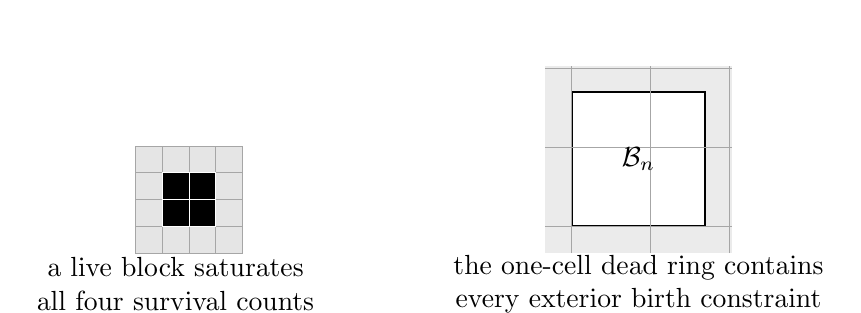
\begin{tikzpicture}[x=.34cm,y=.34cm]
  \begin{scope}
    \foreach \i in {-1,...,2}{\foreach \j in {-1,...,2}{
      \fill[black!10] (\i,\j) rectangle ++(1,1);
      \draw[black!35,line width=.25pt] (\i,\j) rectangle ++(1,1);
    }}
    \foreach \i in {0,1}{\foreach \j in {0,1}{
      \fill[black] (\i,\j) rectangle ++(1,1);
      \draw[white,line width=.25pt] (\i,\j) rectangle ++(1,1);
    }}
    \node[align=center] at (.5,-2.15) {a live block saturates\\all four survival counts};
  \end{scope}
  \begin{scope}[xshift=5.2cm]
    \fill[black!8] (-1,-1) rectangle (6,6);
    \fill[white] (0,0) rectangle (5,5);
    \draw[black,line width=.7pt] (0,0) rectangle (5,5);
    \draw[black!35,line width=.25pt] (-1,-1) grid (6,6);
    \node at (2.5,2.5) {$\B_n$};
    \node[align=center] at (2.5,-2.15) {the one-cell dead ring contains\\every exterior birth constraint};
  \end{scope}
\end{tikzpicture}
\caption{The two local reductions.  The gray cells around the live block
cannot be live; the shaded layer is the complete exterior verification ring.}
\label{fig:local-reductions}
\end{figure}

\subsection{The unrestricted benchmark and wastage}\label{sec:wastage}

\begin{theorem}[Chu--Stuckey]\label{thm:chu}
Every connected still life is unrestricted, so $C(n)\le M(n)$.  The values of
$M(n)$ for $n\le60$ are given by the exact table in~\cite{chu-stuckey-2012};
those used in the ledger appear in \cref{tab:bounds}.  For $n\ge61$, let
\[
\Rminus=\{0,1,3,8,9,11,16,17,19,25,27,31,33,39,41,47,49\}
 \pmod {54}.
\]
Then
\begin{equation}\label{eq:chu-formula}
M(n)=
\begin{cases}
\left\lfloor\dfrac{n^2}{2}+\dfrac{17n}{27}-2\right\rfloor,
 & n\bmod54\in\Rminus,\\[6pt]
\left\lfloor\dfrac{n^2}{2}+\dfrac{17n}{27}-1\right\rfloor,
 & n\bmod54\notin\Rminus.
\end{cases}
\end{equation}
\end{theorem}

Chu and Stuckey redistribute two tokens initially placed at every lattice
cell.  Each live cell receives at least four tokens, and the undistributed
tokens define a nonnegative local wastage.  For a dead centre with
$0,1,2,3,4$ live orthogonal neighbours the preliminary charge is $2,1,0,0,2$; a
live centre is charged for eligible dead orthogonal donors beyond two, with the
four exceptional donor and recipient patterns of~\cite{chu-stuckey-2012}
assigned charge zero.  On a finite dead-exterior square the identity is exact.

\begin{theorem}[Wastage identity]\label{thm:wastage}
For every finite-board still life $S\subseteq\B_n$ there is a sum $W(S)$ of
nonnegative radius-one local charges and side contributions such that
\begin{equation}\label{eq:wastage}
 W(S)=2n^2+4n-4|S|,
 \qquad
 |S|=\frac{2n^2+4n-W(S)}4.
\end{equation}
In particular $W(S)\equiv2n^2+4n\pmod4$.
\end{theorem}

\begin{lemma}[Partial-charge upper bound]\label{lem:partial-charge}
If a set of local terms completely determined by a boundary annulus has total
charge at least $B$, then every full still-life completion satisfies
$|S|\le\lfloor(2n^2+4n-B)/4\rfloor$.
\end{lemma}

\begin{proof}
All omitted wastage terms are nonnegative, so $W(S)\ge B$; substitute in
\eqref{eq:wastage}.
\end{proof}

\section{Boundary automata and a residue-eight upper bound}\label{sec:boundary}

The connected upper bound is a relaxation.  By \cref{cor:block-free} every
relevant connected pattern is block-free, so we minimize wastage over all
locally stable, block-free boundary annuli, without requiring that the annulus
extend to a connected interior.  The relaxed class is larger, so its minimum
charge is a valid lower bound on the charge of every connected board.

\subsection{Straight edges, corners, and min-plus composition}

Fix a depth $h\ge3$.  A straight-edge state is an ordered pair $(a,b)$ of
binary column masks of height $h+2$: the outermost bit is the dead exterior,
the next $h$ bits are the charged boundary strip, and the last bit is an inward
halo.  A transition $(a,b)\to(b,c)$ is admitted exactly when appending $c$
satisfies the Life rule at every centre whose neighbourhood has just become
complete, suppresses births at the exterior centre finalized by the transition,
and creates no live $2\times2$ block.  Its weight is the sum of the newly
finalized local wastage terms.  With $E_h$ the weighted adjacency matrix and
$(A\otimes B)_{ij}=\min_k(A_{ik}+B_{kj})$ the min-plus product, the minimum-cost
length-$L$ path matrix satisfies
\begin{equation}\label{eq:minplus-step}
 D_{h,L+1}=D_{h,L}\otimes E_h.
\end{equation}
A corner is not determined by two independent edge endpoints, so the complete
$(h+1)\times(h+1)$ corner patches are enumerated directly, giving a weighted
corner relation $K_h$.  A depth-$h$ ring has straight length $n-2h$ on each side
and minimum charge
\begin{equation}\label{eq:ring-product}
 B_h(n)=
 \min_{\alpha_j,\beta_j}
 \sum_{j=0}^3
 \left(D_{h,n-2h}(\alpha_j,\beta_j)+K_h(\beta_j,\alpha_{j+1})\right),
 \qquad \alpha_4=\alpha_0.
\end{equation}
Straight strips and corners partition the annular local terms, every full board
projects to a feasible ring, and the uncharged interior terms are nonnegative,
so by \cref{lem:partial-charge}
\begin{equation}\label{eq:Bh-upper}
 C(n)\le
 \left\lfloor\frac{2n^2+4n-B_h(n)}4\right\rfloor.
\end{equation}

\begin{figure}[t]
\centering
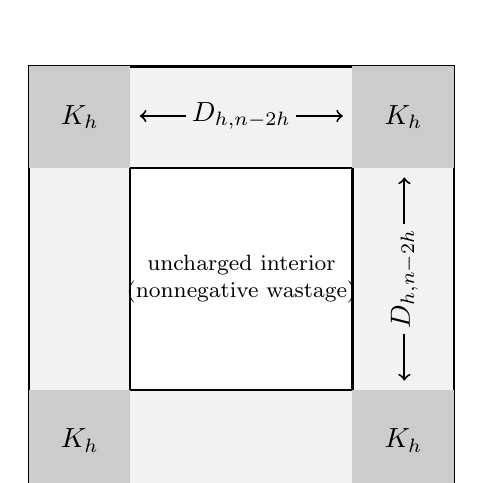
\begin{tikzpicture}[scale=.6]
  \fill[black!5] (0,0) rectangle (9,9);
  \fill[white] (2.15,2.15) rectangle (6.85,6.85);
  \draw[line width=.8pt] (0,0) rectangle (9,9);
  \draw[line width=.8pt] (2.15,2.15) rectangle (6.85,6.85);
  \fill[black!20] (0,6.85) rectangle (2.15,9);
  \fill[black!20] (6.85,6.85) rectangle (9,9);
  \fill[black!20] (6.85,0) rectangle (9,2.15);
  \fill[black!20] (0,0) rectangle (2.15,2.15);
  \draw[<->,line width=.7pt] (2.35,7.95) -- (6.65,7.95)
    node[midway,fill=black!5,inner sep=2pt] {$D_{h,n-2h}$};
  \draw[<->,line width=.7pt] (7.95,6.65) -- (7.95,2.35)
    node[midway,fill=black!5,inner sep=2pt,rotate=90] {$D_{h,n-2h}$};
  \node at (1.08,7.93) {$K_h$};
  \node at (7.93,7.93) {$K_h$};
  \node at (7.93,1.08) {$K_h$};
  \node at (1.08,1.08) {$K_h$};
  \node[align=center,font=\footnotesize] at (4.5,4.5) {uncharged interior\\(nonnegative wastage)};
\end{tikzpicture}
\caption{The square boundary as a cyclic min-plus product of four straight path
matrices and four corner relations.}
\label{fig:ring-automaton}
\end{figure}

The finite certificates rest on an entrywise matrix recurrence, not on a
recurrence for the scalar minimum.

\begin{lemma}[Propagation of a min-plus period]\label{lem:minplus-period}
If $D_{h,L_0+p}=D_{h,L_0}+\delta$ entrywise, including equality of the
$+\infty$ pattern, then $D_{h,L+p}=D_{h,L}+\delta$ for all $L\ge L_0$.
\end{lemma}

\begin{proof}
By \eqref{eq:minplus-step},
$D_{h,L_0+p+1}=(D_{h,L_0}+\delta)\otimes E_h=D_{h,L_0+1}+\delta$, and the
argument iterates; equality of the infinite entries preserves reachability.
\end{proof}

Since the corner relation is fixed, an entrywise side recurrence passes through
\eqref{eq:ring-product}: increasing $n$ by eight increases the four-side minimum
by $4\cdot3=12$.

\subsection{The bound}

At depth three the block-free edge graph has 214 states and 771 arcs, and an
integer potential $p$ on its states satisfies $8w(e)-3+p(s)-p(t)\ge0$ for every
arc $e:s\to t$ of wastage $w(e)$; summing around a cycle shows that every cycle
has mean weight at least $3/8$, and length-eight cycles of cost three attain it.
Together with the complete $4\times4$ corner census and the entrywise recurrence
$D_{3,L+8}=D_{3,L}+3$ for $L\ge20$, this gives the depth-three bound.  Depth
four retains one more inward layer.  The certificate data for depths three
through six are listed in \cref{app:boundary}.

\begin{proposition}[Depths three and four]\label{prop:U4}
For $n\ge10$ and $n\ge14$ respectively,
\[
 C(n)\le U_3(n)=\left\lfloor\frac{4n^2+5n-b_{n\bmod8}}8\right\rfloor,
 \qquad
 C(n)\le U_4(n)=\left\lfloor\frac{4n^2+5n-c_{n\bmod8}}8\right\rfloor,
\]
where $(b_0,\ldots,b_7)=(18,15,10,15,12,15,18,3)$ and
$(c_0,\ldots,c_7)=(18,23,18,23,20,15,26,11)$.
\end{proposition}

Residues zero and five require equality-language arguments.  At depth five the
minima at $n=21,29,37,45,53$ are one unit above the depth-four charges, and the
restricted matrix recurrence propagates the improvement.  For residue zero, the
equality rings of depth five lie in a small support, and a safe depth-six lift
of that support, which keeps every valid incoming and outgoing edge and both
choices of the new halo bit, contains no ring at the old target for
$n=16,24,32,40$; the restricted matrix again increases entrywise by three.

\begin{proposition}[Residues five and zero]\label{prop:residue}
If $n\ge21$ and $n\equiv5\pmod8$, then $C(n)\le U_4(n)-1$.  If $n\ge16$ and
$n\equiv0\pmod8$, then $C(n)\le U_3(n)-1$.
\end{proposition}

\begin{theorem}[Connected boundary upper bound]\label{thm:upper}
For every $n\ge14$, $C(n)\le U(n)$ with $U$ as in \eqref{eq:main-upper} and $d$
as in \eqref{eq:d-vector}.  Therefore $C(n)\le\min\{M(n),U(n)\}$.
\end{theorem}

\begin{proof}
Use $U_4$ in residues $1,2,3,4,6,7$.  In residue five, subtracting one from
$U_4$ changes $c_5=15$ to $d_5=23$; in residue zero, subtracting one from $U_3$
changes $b_0=18$ to $d_0=26$.  The unrestricted inequality is \cref{thm:chu}.
\end{proof}

\begin{corollary}[Upper-bound recurrence]\label{cor:U-recurrence}
For every $n\ge14$, $U(n+8)=U(n)+8n+37$.
\end{corollary}

\begin{proof}
The residue correction is unchanged, and $4(n+8)^2+5(n+8)-(4n^2+5n)=8(8n+37)$
is divisible by eight, so the increment passes through the floor.
\end{proof}

This is a recurrence for a proved upper bound, not for $C(n)$: boundary
feasibility does not guarantee a connected interior completion.

\section{Exact values}\label{sec:exact}

The exact values of \cref{thm:main} are closed by the arguments of
\cref{tab:exact-methods}.  In every row the lower bound is a verified connected
board.  The proof index of the accompanying repository~\cite{repo} records, for
some small sizes, further independent routes: equality with $M(n)$ at
$n=2,3,4,6,7,9$ and complete block-free row enumerations at $n=5,8,10,11$.

\begin{table}[!htbp]
\centering
\caption{Upper-bound method for each exact value.}
\label{tab:exact-methods}
\small
\begin{tabularx}{\textwidth}{@{}>{\raggedright\arraybackslash}p{0.2\textwidth} >{\raggedright\arraybackslash}p{0.3\textwidth} X@{}}
\toprule
sizes & exact values & upper-bound mechanism \\
\midrule
$1$ & $0$ & a single live cell dies \\
$2$--$11$ & $4,6,8,11,18,28,32,43,53,63$ & complete connected threshold encodings with proof-logged refutations (\cref{app:sat}) \\
$12,15,20,23,31,39$ & $76,119,210,276,497,782$ & connected boards attain $M(n)$ \\
$13$ & $88$ & exhaustive block-free row dynamic program (\cref{app:n13}) \\
$14$ & $102$ & complete depth-four low-wastage belt enumeration (\cref{app:n14}) \\
$16,21,24,25,29,32,33$ & $134,230,299,325,435,528,562$ & connected boards attain $U(n)$ \\
$37,41,45,49,53,57,65$ & $704,863,1037,1228,1434,1657,2150$ & connected boards attain $U(n)$ \\
$17$ & $151$ & depth-five equality support and zero-charge depth-six lift (\cref{app:n17}) \\
$18$ & $170$ & depth-seven exclusion of population $171$ (\cref{app:n18}) \\
$19$ & $188$ & depth-nine exclusion of population $189$ (\cref{app:n19}) \\
$22$ & $251$ & depth-eleven exclusion of population $252$ (\cref{app:n22}) \\
\bottomrule
\end{tabularx}
\end{table}

\subsection{Closures by the unrestricted optimum and by the boundary bound}
\label{sec:closures-U}

At $n=12,15,20,23,31,39$ connected boards attain
$M(n)=76,119,210,276,497,782$, so $C(n)=M(n)$ there.  At $n=23,31,39$ the
boundary formula is one cell weaker, since $U(23)=277$, $U(31)=498$, and
$U(39)=783$.  Elsewhere the boundary bound is attained.

\begin{proposition}[Closure by the boundary bound]\label{prop:closure-U}
For $n\in\{16,21,24,25,29,32,33,37,41,45,49,53,57,65\}$ there is a verified
connected still life in $\B_n$ of population $U(n)$, so $C(n)=U(n)$:
\[
\begin{array}{c|cccccccccccccc}
n&16&21&24&25&29&32&33&37&41&45&49&53&57&65\\
\hline
C(n)&134&230&299&325&435&528&562&704&863&1037&1228&1434&1657&2150
\end{array}
\]
\end{proposition}

\begin{proof}
By \cref{thm:upper}, $C(n)\le U(n)$ for $n\ge14$, and each listed board has
exactly $U(n)$ live cells, is stable on $\B_n\cup R_n$, and has one Moore
component.  These properties are recomputed by the audit script of
\cref{app:certificates}.
\end{proof}

The exact values with $n\equiv5\pmod8$, $21\le n\le53$, and with
$n\equiv1\pmod8$, $25\le n\le65$, form the chains
\[
 21\to29\to37\to45\to53
 \qquad\text{and}\qquad
 25\to33\to41\to49\to57\to65,
\]
in which consecutive values differ by exactly $8n+37$, the increment of $U$ in
\cref{cor:U-recurrence}; for example $C(65)=2150=1657+8\cdot57+37$.  These are
finite verified chains, not a proof that they continue.

\subsection{Specialized closures}\label{sec:special}

The remaining exact values need finite arguments beyond
\cref{thm:upper}.  We summarize them here; the complete arguments are in
\cref{app:closures}.

\begin{itemize}[leftmargin=1.2em,label={}]
\item \emph{$n\le11$.} Complete threshold encodings with a rooted spanning-tree
connectivity model; unsatisfiability at $C(n)+1$ is certified by replayed
proofs.
\item \emph{$n=13$.} Any connected board with 89 cells is block-free; an exhaustive
block-free row dynamic program, over 3,926,925,326 transitions, has maximum 88.
\item \emph{$n=14$.} A 103-cell board would have wastage 36; all 261,225 physical
low-charge depth-four belts and their centre completions give 224 stable
103-cell boards, none connected.
\item \emph{$n=16,17$.} A corrected depth-six charge with the wastage congruence gives
$C(16)\le134$; at $n=17$ the depth-five equality support for wastage $38$ has a
safe depth-six lift of minimum cost $39$, excluding 152.
\item \emph{$n=18,19,22$.} Here $U(n)$ is one cell too weak.  For the target
population $P=U(n)$ the wastage is $W=2n^2+4n-4P$, and the complete set of
boundary rings of charge at most $W$ is lifted inward, layer by layer, keeping
every physical corner and extension that could still spend the remaining
slack.  The set becomes empty at depth seven for $n=18$ ($W=36$), at depth nine
for $n=19$ ($W=42$), and at depth eleven for $n=22$ ($W=48$), where the
straight sides have length zero.  Verified boards of populations 170, 188, and
251 meet the resulting bounds.  The 170-cell board at $n=18$ does not come from
component repair of the unrestricted optimum, where all 170-cell repairs have
three components; it was recovered from the complete low-slack boundary
language, and it is checked directly.
\end{itemize}

\begin{figure}[t]
\centering
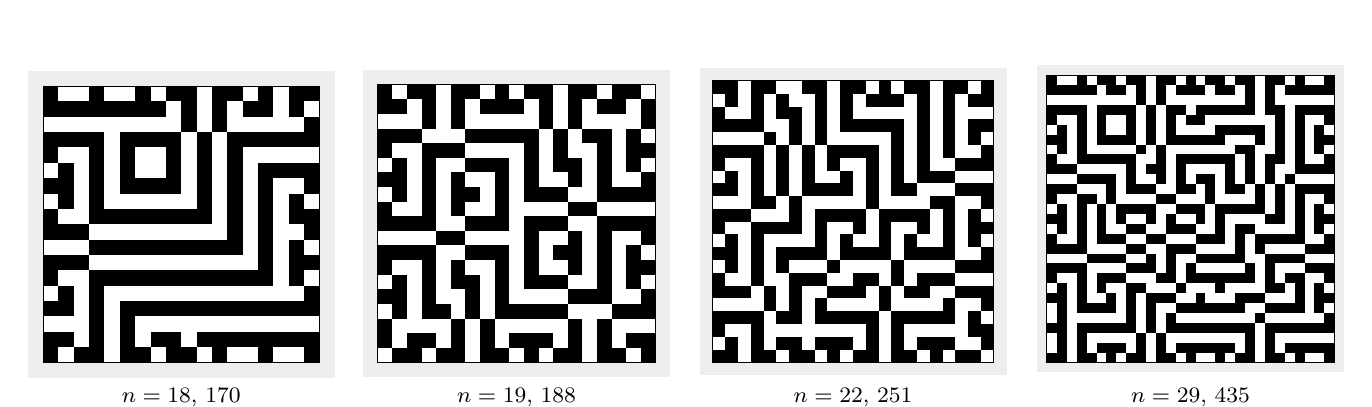
\begin{tikzpicture}
\begin{scope}[xshift=0.000cm]
\begin{scope}[x=0.1950cm,y=0.1950cm]
\fill[black!7] (-1,-1) rectangle (19,19);
\fill[white] (0,0) rectangle (18,18);
\draw[black,line width=.35pt] (0,0) rectangle (18,18);
\fill (0,17) rectangle (1,18);
\fill (3,17) rectangle (4,18);
\fill (6,17) rectangle (7,18);
\fill (8,17) rectangle (10,18);
\fill (11,17) rectangle (13,18);
\fill (14,17) rectangle (15,18);
\fill (16,17) rectangle (18,18);
\fill (0,16) rectangle (8,17);
\fill (9,16) rectangle (10,17);
\fill (11,16) rectangle (12,17);
\fill (13,16) rectangle (15,17);
\fill (16,16) rectangle (17,17);
\fill (9,15) rectangle (10,16);
\fill (11,15) rectangle (12,16);
\fill (17,15) rectangle (18,16);
\fill (0,14) rectangle (4,15);
\fill (5,14) rectangle (9,15);
\fill (10,14) rectangle (11,15);
\fill (12,14) rectangle (18,15);
\fill (0,13) rectangle (1,14);
\fill (3,13) rectangle (4,14);
\fill (5,13) rectangle (6,14);
\fill (8,13) rectangle (9,14);
\fill (10,13) rectangle (11,14);
\fill (12,13) rectangle (13,14);
\fill (1,12) rectangle (2,13);
\fill (3,12) rectangle (4,13);
\fill (5,12) rectangle (6,13);
\fill (8,12) rectangle (9,13);
\fill (10,12) rectangle (11,13);
\fill (12,12) rectangle (13,13);
\fill (14,12) rectangle (18,13);
\fill (0,11) rectangle (2,12);
\fill (3,11) rectangle (4,12);
\fill (5,11) rectangle (9,12);
\fill (10,11) rectangle (11,12);
\fill (12,11) rectangle (13,12);
\fill (14,11) rectangle (15,12);
\fill (17,11) rectangle (18,12);
\fill (1,10) rectangle (2,11);
\fill (3,10) rectangle (4,11);
\fill (10,10) rectangle (11,11);
\fill (12,10) rectangle (13,11);
\fill (14,10) rectangle (15,11);
\fill (16,10) rectangle (17,11);
\fill (0,9) rectangle (1,10);
\fill (3,9) rectangle (11,10);
\fill (12,9) rectangle (13,10);
\fill (14,9) rectangle (15,10);
\fill (16,9) rectangle (18,10);
\fill (0,8) rectangle (3,9);
\fill (12,8) rectangle (13,9);
\fill (14,8) rectangle (15,9);
\fill (17,8) rectangle (18,9);
\fill (3,7) rectangle (13,8);
\fill (14,7) rectangle (15,8);
\fill (16,7) rectangle (17,8);
\fill (0,6) rectangle (3,7);
\fill (14,6) rectangle (15,7);
\fill (16,6) rectangle (18,7);
\fill (0,5) rectangle (1,6);
\fill (3,5) rectangle (15,6);
\fill (16,5) rectangle (17,6);
\fill (1,4) rectangle (2,5);
\fill (3,4) rectangle (4,5);
\fill (17,4) rectangle (18,5);
\fill (0,3) rectangle (2,4);
\fill (3,3) rectangle (4,4);
\fill (5,3) rectangle (18,4);
\fill (3,2) rectangle (4,3);
\fill (5,2) rectangle (6,3);
\fill (0,1) rectangle (2,2);
\fill (3,1) rectangle (4,2);
\fill (5,1) rectangle (6,2);
\fill (7,1) rectangle (9,2);
\fill (10,1) rectangle (18,2);
\fill (0,0) rectangle (1,1);
\fill (2,0) rectangle (4,1);
\fill (5,0) rectangle (7,1);
\fill (8,0) rectangle (10,1);
\fill (11,0) rectangle (12,1);
\fill (14,0) rectangle (15,1);
\fill (17,0) rectangle (18,1);
\end{scope}
\node[align=center,font=\footnotesize] at (1.755,-0.45) {$n=18$, $170$};
\end{scope}
\begin{scope}[xshift=4.250cm]
\begin{scope}[x=0.1857cm,y=0.1857cm]
\fill[black!7] (-1,-1) rectangle (20,20);
\fill[white] (0,0) rectangle (19,19);
\draw[black,line width=.35pt] (0,0) rectangle (19,19);
\fill (0,18) rectangle (1,19);
\fill (2,18) rectangle (4,19);
\fill (5,18) rectangle (7,19);
\fill (8,18) rectangle (9,19);
\fill (10,18) rectangle (12,19);
\fill (13,18) rectangle (15,19);
\fill (16,18) rectangle (18,19);
\fill (0,17) rectangle (2,18);
\fill (3,17) rectangle (4,18);
\fill (5,17) rectangle (6,18);
\fill (7,17) rectangle (10,18);
\fill (11,17) rectangle (12,18);
\fill (13,17) rectangle (14,18);
\fill (15,17) rectangle (17,18);
\fill (18,17) rectangle (19,18);
\fill (3,16) rectangle (4,17);
\fill (5,16) rectangle (6,17);
\fill (11,16) rectangle (12,17);
\fill (13,16) rectangle (14,17);
\fill (18,16) rectangle (19,17);
\fill (0,15) rectangle (3,16);
\fill (6,15) rectangle (11,16);
\fill (12,15) rectangle (13,16);
\fill (14,15) rectangle (16,16);
\fill (17,15) rectangle (18,16);
\fill (0,14) rectangle (1,15);
\fill (3,14) rectangle (6,15);
\fill (10,14) rectangle (11,15);
\fill (12,14) rectangle (13,15);
\fill (15,14) rectangle (16,15);
\fill (17,14) rectangle (19,15);
\fill (1,13) rectangle (2,14);
\fill (3,13) rectangle (4,14);
\fill (6,13) rectangle (9,14);
\fill (10,13) rectangle (11,14);
\fill (12,13) rectangle (14,14);
\fill (15,13) rectangle (16,14);
\fill (17,13) rectangle (18,14);
\fill (0,12) rectangle (2,13);
\fill (3,12) rectangle (4,13);
\fill (5,12) rectangle (6,13);
\fill (8,12) rectangle (9,13);
\fill (10,12) rectangle (11,13);
\fill (13,12) rectangle (14,13);
\fill (15,12) rectangle (16,13);
\fill (18,12) rectangle (19,13);
\fill (1,11) rectangle (2,12);
\fill (3,11) rectangle (4,12);
\fill (5,11) rectangle (7,12);
\fill (8,11) rectangle (9,12);
\fill (10,11) rectangle (13,12);
\fill (15,11) rectangle (19,12);
\fill (0,10) rectangle (1,11);
\fill (3,10) rectangle (4,11);
\fill (5,10) rectangle (6,11);
\fill (8,10) rectangle (9,11);
\fill (13,10) rectangle (15,11);
\fill (0,9) rectangle (4,10);
\fill (6,9) rectangle (9,10);
\fill (10,9) rectangle (13,10);
\fill (15,9) rectangle (19,10);
\fill (4,8) rectangle (6,9);
\fill (10,8) rectangle (11,9);
\fill (13,8) rectangle (14,9);
\fill (15,8) rectangle (16,9);
\fill (18,8) rectangle (19,9);
\fill (0,7) rectangle (4,8);
\fill (6,7) rectangle (9,8);
\fill (10,7) rectangle (11,8);
\fill (12,7) rectangle (14,8);
\fill (15,7) rectangle (16,8);
\fill (17,7) rectangle (18,8);
\fill (0,6) rectangle (1,7);
\fill (3,6) rectangle (4,7);
\fill (5,6) rectangle (6,7);
\fill (8,6) rectangle (9,7);
\fill (10,6) rectangle (11,7);
\fill (13,6) rectangle (14,7);
\fill (15,6) rectangle (16,7);
\fill (17,6) rectangle (19,7);
\fill (1,5) rectangle (2,6);
\fill (3,5) rectangle (4,6);
\fill (5,5) rectangle (7,6);
\fill (8,5) rectangle (9,6);
\fill (10,5) rectangle (13,6);
\fill (15,5) rectangle (16,6);
\fill (17,5) rectangle (18,6);
\fill (0,4) rectangle (2,5);
\fill (3,4) rectangle (4,5);
\fill (6,4) rectangle (7,5);
\fill (8,4) rectangle (9,5);
\fill (13,4) rectangle (16,5);
\fill (18,4) rectangle (19,5);
\fill (1,3) rectangle (2,4);
\fill (3,3) rectangle (5,4);
\fill (6,3) rectangle (7,4);
\fill (8,3) rectangle (13,4);
\fill (16,3) rectangle (19,4);
\fill (0,2) rectangle (1,3);
\fill (5,2) rectangle (6,3);
\fill (7,2) rectangle (8,3);
\fill (13,2) rectangle (14,3);
\fill (15,2) rectangle (16,3);
\fill (0,1) rectangle (1,2);
\fill (2,1) rectangle (4,2);
\fill (5,1) rectangle (6,2);
\fill (7,1) rectangle (8,2);
\fill (9,1) rectangle (12,2);
\fill (13,1) rectangle (14,2);
\fill (15,1) rectangle (16,2);
\fill (17,1) rectangle (19,2);
\fill (1,0) rectangle (3,1);
\fill (4,0) rectangle (6,1);
\fill (7,0) rectangle (9,1);
\fill (10,0) rectangle (11,1);
\fill (12,0) rectangle (14,1);
\fill (15,0) rectangle (17,1);
\fill (18,0) rectangle (19,1);
\end{scope}
\node[align=center,font=\footnotesize] at (1.764,-0.45) {$n=19$, $188$};
\end{scope}
\begin{scope}[xshift=8.500cm]
\begin{scope}[x=0.1625cm,y=0.1625cm]
\fill[black!7] (-1,-1) rectangle (23,23);
\fill[white] (0,0) rectangle (22,22);
\draw[black,line width=.35pt] (0,0) rectangle (22,22);
\fill (0,21) rectangle (2,22);
\fill (3,21) rectangle (5,22);
\fill (7,21) rectangle (9,22);
\fill (10,21) rectangle (12,22);
\fill (13,21) rectangle (14,22);
\fill (15,21) rectangle (17,22);
\fill (18,21) rectangle (20,22);
\fill (21,21) rectangle (22,22);
\fill (1,20) rectangle (2,21);
\fill (3,20) rectangle (4,21);
\fill (5,20) rectangle (6,21);
\fill (8,20) rectangle (9,21);
\fill (10,20) rectangle (11,21);
\fill (12,20) rectangle (15,21);
\fill (16,20) rectangle (17,21);
\fill (18,20) rectangle (19,21);
\fill (20,20) rectangle (22,21);
\fill (0,19) rectangle (1,20);
\fill (3,19) rectangle (4,20);
\fill (5,19) rectangle (7,20);
\fill (8,19) rectangle (9,20);
\fill (10,19) rectangle (11,20);
\fill (16,19) rectangle (17,20);
\fill (18,19) rectangle (19,20);
\fill (0,18) rectangle (4,19);
\fill (6,18) rectangle (7,19);
\fill (8,18) rectangle (9,19);
\fill (10,18) rectangle (15,19);
\fill (16,18) rectangle (17,19);
\fill (18,18) rectangle (19,19);
\fill (20,18) rectangle (22,19);
\fill (4,17) rectangle (5,18);
\fill (6,17) rectangle (7,18);
\fill (8,17) rectangle (9,18);
\fill (14,17) rectangle (15,18);
\fill (16,17) rectangle (17,18);
\fill (18,17) rectangle (19,18);
\fill (20,17) rectangle (21,18);
\fill (0,16) rectangle (4,17);
\fill (5,16) rectangle (6,17);
\fill (7,16) rectangle (8,17);
\fill (9,16) rectangle (13,17);
\fill (14,16) rectangle (15,17);
\fill (16,16) rectangle (17,17);
\fill (18,16) rectangle (19,17);
\fill (21,16) rectangle (22,17);
\fill (0,15) rectangle (1,16);
\fill (3,15) rectangle (4,16);
\fill (5,15) rectangle (6,16);
\fill (7,15) rectangle (8,16);
\fill (9,15) rectangle (10,16);
\fill (12,15) rectangle (13,16);
\fill (14,15) rectangle (15,16);
\fill (16,15) rectangle (17,16);
\fill (19,15) rectangle (22,16);
\fill (1,14) rectangle (2,15);
\fill (3,14) rectangle (4,15);
\fill (5,14) rectangle (6,15);
\fill (7,14) rectangle (8,15);
\fill (10,14) rectangle (11,15);
\fill (12,14) rectangle (13,15);
\fill (14,14) rectangle (15,15);
\fill (16,14) rectangle (19,15);
\fill (0,13) rectangle (2,14);
\fill (3,13) rectangle (4,14);
\fill (5,13) rectangle (6,14);
\fill (7,13) rectangle (11,14);
\fill (12,13) rectangle (13,14);
\fill (14,13) rectangle (16,14);
\fill (19,13) rectangle (22,14);
\fill (3,12) rectangle (5,13);
\fill (6,12) rectangle (7,13);
\fill (12,12) rectangle (13,13);
\fill (17,12) rectangle (19,13);
\fill (21,12) rectangle (22,13);
\fill (0,11) rectangle (3,12);
\fill (6,11) rectangle (7,12);
\fill (8,11) rectangle (12,12);
\fill (13,11) rectangle (17,12);
\fill (18,11) rectangle (19,12);
\fill (20,11) rectangle (21,12);
\fill (0,10) rectangle (1,11);
\fill (3,10) rectangle (7,11);
\fill (8,10) rectangle (9,11);
\fill (11,10) rectangle (12,11);
\fill (13,10) rectangle (14,11);
\fill (16,10) rectangle (17,11);
\fill (18,10) rectangle (19,11);
\fill (20,10) rectangle (22,11);
\fill (1,9) rectangle (2,10);
\fill (3,9) rectangle (4,10);
\fill (8,9) rectangle (9,10);
\fill (10,9) rectangle (11,10);
\fill (13,9) rectangle (14,10);
\fill (15,9) rectangle (16,10);
\fill (18,9) rectangle (19,10);
\fill (20,9) rectangle (21,10);
\fill (0,8) rectangle (2,9);
\fill (3,8) rectangle (4,9);
\fill (5,8) rectangle (9,9);
\fill (10,8) rectangle (14,9);
\fill (15,8) rectangle (19,9);
\fill (21,8) rectangle (22,9);
\fill (1,7) rectangle (2,8);
\fill (3,7) rectangle (4,8);
\fill (5,7) rectangle (6,8);
\fill (9,7) rectangle (10,8);
\fill (14,7) rectangle (15,8);
\fill (19,7) rectangle (22,8);
\fill (0,6) rectangle (1,7);
\fill (3,6) rectangle (4,7);
\fill (6,6) rectangle (9,7);
\fill (11,6) rectangle (13,7);
\fill (14,6) rectangle (15,7);
\fill (16,6) rectangle (19,7);
\fill (0,5) rectangle (3,6);
\fill (4,5) rectangle (5,6);
\fill (6,5) rectangle (7,6);
\fill (9,5) rectangle (12,6);
\fill (13,5) rectangle (14,6);
\fill (15,5) rectangle (17,6);
\fill (19,5) rectangle (22,6);
\fill (4,4) rectangle (5,5);
\fill (6,4) rectangle (7,5);
\fill (8,4) rectangle (9,5);
\fill (13,4) rectangle (14,5);
\fill (18,4) rectangle (19,5);
\fill (21,4) rectangle (22,5);
\fill (0,3) rectangle (4,4);
\fill (5,3) rectangle (7,4);
\fill (8,3) rectangle (13,4);
\fill (14,3) rectangle (19,4);
\fill (20,3) rectangle (21,4);
\fill (0,2) rectangle (1,3);
\fill (3,2) rectangle (4,3);
\fill (12,2) rectangle (13,3);
\fill (14,2) rectangle (15,3);
\fill (20,2) rectangle (22,3);
\fill (1,1) rectangle (2,2);
\fill (3,1) rectangle (4,2);
\fill (5,1) rectangle (7,2);
\fill (8,1) rectangle (11,2);
\fill (12,1) rectangle (13,2);
\fill (14,1) rectangle (15,2);
\fill (16,1) rectangle (19,2);
\fill (21,1) rectangle (22,2);
\fill (0,0) rectangle (2,1);
\fill (3,0) rectangle (5,1);
\fill (6,0) rectangle (8,1);
\fill (9,0) rectangle (10,1);
\fill (11,0) rectangle (13,1);
\fill (14,0) rectangle (16,1);
\fill (17,0) rectangle (18,1);
\fill (19,0) rectangle (21,1);
\end{scope}
\node[align=center,font=\footnotesize] at (1.787,-0.45) {$n=22$, $251$};
\end{scope}
\begin{scope}[xshift=12.750cm]
\begin{scope}[x=0.1258cm,y=0.1258cm]
\fill[black!7] (-1,-1) rectangle (30,30);
\fill[white] (0,0) rectangle (29,29);
\draw[black,line width=.35pt] (0,0) rectangle (29,29);
\fill (0,28) rectangle (1,29);
\fill (3,28) rectangle (4,29);
\fill (5,28) rectangle (7,29);
\fill (8,28) rectangle (10,29);
\fill (11,28) rectangle (13,29);
\fill (14,28) rectangle (15,29);
\fill (16,28) rectangle (18,29);
\fill (19,28) rectangle (21,29);
\fill (22,28) rectangle (24,29);
\fill (25,28) rectangle (26,29);
\fill (28,28) rectangle (29,29);
\fill (0,27) rectangle (5,28);
\fill (6,27) rectangle (8,28);
\fill (9,27) rectangle (10,28);
\fill (11,27) rectangle (12,28);
\fill (13,27) rectangle (16,28);
\fill (17,27) rectangle (19,28);
\fill (20,27) rectangle (21,28);
\fill (22,27) rectangle (23,28);
\fill (24,27) rectangle (29,28);
\fill (9,26) rectangle (10,27);
\fill (11,26) rectangle (12,27);
\fill (20,26) rectangle (21,27);
\fill (22,26) rectangle (23,27);
\fill (0,25) rectangle (4,26);
\fill (5,25) rectangle (9,26);
\fill (10,25) rectangle (11,26);
\fill (12,25) rectangle (14,26);
\fill (15,25) rectangle (21,26);
\fill (22,25) rectangle (24,26);
\fill (25,25) rectangle (29,26);
\fill (0,24) rectangle (1,25);
\fill (3,24) rectangle (4,25);
\fill (5,24) rectangle (6,25);
\fill (8,24) rectangle (9,25);
\fill (10,24) rectangle (11,25);
\fill (12,24) rectangle (13,25);
\fill (14,24) rectangle (16,25);
\fill (23,24) rectangle (24,25);
\fill (25,24) rectangle (26,25);
\fill (28,24) rectangle (29,25);
\fill (1,23) rectangle (2,24);
\fill (3,23) rectangle (4,24);
\fill (5,23) rectangle (6,24);
\fill (8,23) rectangle (9,24);
\fill (10,23) rectangle (11,24);
\fill (12,23) rectangle (13,24);
\fill (17,23) rectangle (22,24);
\fill (23,23) rectangle (24,24);
\fill (25,23) rectangle (26,24);
\fill (27,23) rectangle (28,24);
\fill (0,22) rectangle (2,23);
\fill (3,22) rectangle (4,23);
\fill (5,22) rectangle (9,23);
\fill (10,22) rectangle (11,23);
\fill (12,22) rectangle (18,23);
\fill (21,22) rectangle (22,23);
\fill (23,22) rectangle (24,23);
\fill (25,22) rectangle (26,23);
\fill (27,22) rectangle (29,23);
\fill (1,21) rectangle (2,22);
\fill (3,21) rectangle (4,22);
\fill (9,21) rectangle (10,22);
\fill (11,21) rectangle (12,22);
\fill (19,21) rectangle (21,22);
\fill (23,21) rectangle (24,22);
\fill (25,21) rectangle (26,22);
\fill (27,21) rectangle (28,22);
\fill (0,20) rectangle (1,21);
\fill (3,20) rectangle (9,21);
\fill (11,20) rectangle (12,21);
\fill (13,20) rectangle (19,21);
\fill (20,20) rectangle (21,21);
\fill (22,20) rectangle (24,21);
\fill (25,20) rectangle (26,21);
\fill (28,20) rectangle (29,21);
\fill (0,19) rectangle (3,20);
\fill (8,19) rectangle (9,20);
\fill (10,19) rectangle (12,20);
\fill (13,19) rectangle (14,20);
\fill (18,19) rectangle (19,20);
\fill (20,19) rectangle (21,20);
\fill (22,19) rectangle (23,20);
\fill (25,19) rectangle (29,20);
\fill (3,18) rectangle (7,19);
\fill (8,18) rectangle (9,19);
\fill (11,18) rectangle (12,19);
\fill (13,18) rectangle (14,19);
\fill (15,18) rectangle (17,19);
\fill (18,18) rectangle (19,19);
\fill (20,18) rectangle (21,19);
\fill (22,18) rectangle (23,19);
\fill (24,18) rectangle (25,19);
\fill (0,17) rectangle (3,18);
\fill (6,17) rectangle (7,18);
\fill (8,17) rectangle (11,18);
\fill (13,17) rectangle (15,18);
\fill (16,17) rectangle (17,18);
\fill (18,17) rectangle (20,18);
\fill (21,17) rectangle (22,18);
\fill (23,17) rectangle (24,18);
\fill (25,17) rectangle (29,18);
\fill (0,16) rectangle (1,17);
\fill (3,16) rectangle (5,17);
\fill (6,16) rectangle (7,17);
\fill (11,16) rectangle (13,17);
\fill (16,16) rectangle (17,17);
\fill (21,16) rectangle (22,17);
\fill (23,16) rectangle (24,17);
\fill (25,16) rectangle (26,17);
\fill (28,16) rectangle (29,17);
\fill (1,15) rectangle (2,16);
\fill (3,15) rectangle (4,16);
\fill (5,15) rectangle (6,16);
\fill (7,15) rectangle (11,16);
\fill (13,15) rectangle (16,16);
\fill (17,15) rectangle (22,16);
\fill (23,15) rectangle (24,16);
\fill (25,15) rectangle (26,16);
\fill (27,15) rectangle (28,16);
\fill (0,14) rectangle (2,15);
\fill (3,14) rectangle (4,15);
\fill (5,14) rectangle (6,15);
\fill (7,14) rectangle (8,15);
\fill (10,14) rectangle (11,15);
\fill (12,14) rectangle (13,15);
\fill (15,14) rectangle (16,15);
\fill (17,14) rectangle (18,15);
\fill (22,14) rectangle (24,15);
\fill (25,14) rectangle (26,15);
\fill (27,14) rectangle (29,15);
\fill (1,13) rectangle (2,14);
\fill (3,13) rectangle (4,14);
\fill (5,13) rectangle (6,14);
\fill (8,13) rectangle (10,14);
\fill (12,13) rectangle (15,14);
\fill (17,13) rectangle (18,14);
\fill (19,13) rectangle (21,14);
\fill (25,13) rectangle (26,14);
\fill (27,13) rectangle (28,14);
\fill (0,12) rectangle (1,13);
\fill (3,12) rectangle (4,13);
\fill (5,12) rectangle (8,13);
\fill (10,12) rectangle (12,13);
\fill (15,12) rectangle (18,13);
\fill (19,12) rectangle (20,13);
\fill (21,12) rectangle (26,13);
\fill (28,12) rectangle (29,13);
\fill (0,11) rectangle (4,12);
\fill (8,11) rectangle (10,12);
\fill (12,11) rectangle (15,12);
\fill (19,11) rectangle (20,12);
\fill (21,11) rectangle (22,12);
\fill (26,11) rectangle (29,12);
\fill (4,10) rectangle (8,11);
\fill (10,10) rectangle (11,11);
\fill (12,10) rectangle (13,11);
\fill (15,10) rectangle (20,11);
\fill (22,10) rectangle (26,11);
\fill (0,9) rectangle (4,10);
\fill (8,9) rectangle (11,10);
\fill (12,9) rectangle (13,10);
\fill (14,9) rectangle (15,10);
\fill (20,9) rectangle (21,10);
\fill (22,9) rectangle (23,10);
\fill (26,9) rectangle (29,10);
\fill (0,8) rectangle (1,9);
\fill (3,8) rectangle (4,9);
\fill (5,8) rectangle (8,9);
\fill (11,8) rectangle (13,9);
\fill (14,8) rectangle (21,9);
\fill (22,8) rectangle (23,9);
\fill (24,8) rectangle (26,9);
\fill (28,8) rectangle (29,9);
\fill (1,7) rectangle (2,8);
\fill (3,7) rectangle (4,8);
\fill (5,7) rectangle (6,8);
\fill (8,7) rectangle (10,8);
\fill (13,7) rectangle (14,8);
\fill (17,7) rectangle (18,8);
\fill (22,7) rectangle (24,8);
\fill (25,7) rectangle (26,8);
\fill (27,7) rectangle (28,8);
\fill (0,6) rectangle (2,7);
\fill (3,6) rectangle (4,7);
\fill (6,6) rectangle (7,7);
\fill (8,6) rectangle (9,7);
\fill (10,6) rectangle (13,7);
\fill (15,6) rectangle (16,7);
\fill (19,6) rectangle (22,7);
\fill (25,6) rectangle (26,7);
\fill (27,6) rectangle (29,7);
\fill (1,5) rectangle (2,6);
\fill (3,5) rectangle (7,6);
\fill (8,5) rectangle (9,6);
\fill (10,5) rectangle (11,6);
\fill (13,5) rectangle (20,6);
\fill (22,5) rectangle (26,6);
\fill (27,5) rectangle (28,6);
\fill (1,4) rectangle (2,5);
\fill (8,4) rectangle (9,5);
\fill (10,4) rectangle (11,5);
\fill (12,4) rectangle (13,5);
\fill (21,4) rectangle (22,5);
\fill (28,4) rectangle (29,5);
\fill (0,3) rectangle (2,4);
\fill (3,3) rectangle (9,4);
\fill (10,3) rectangle (11,4);
\fill (12,3) rectangle (21,4);
\fill (22,3) rectangle (29,4);
\fill (1,2) rectangle (2,3);
\fill (3,2) rectangle (4,3);
\fill (9,2) rectangle (10,3);
\fill (11,2) rectangle (12,3);
\fill (20,2) rectangle (21,3);
\fill (22,2) rectangle (23,3);
\fill (1,1) rectangle (2,2);
\fill (3,1) rectangle (4,2);
\fill (5,1) rectangle (8,2);
\fill (9,1) rectangle (10,2);
\fill (11,1) rectangle (12,2);
\fill (13,1) rectangle (19,2);
\fill (20,1) rectangle (21,2);
\fill (22,1) rectangle (23,2);
\fill (24,1) rectangle (29,2);
\fill (0,0) rectangle (2,1);
\fill (3,0) rectangle (5,1);
\fill (6,0) rectangle (7,1);
\fill (8,0) rectangle (10,1);
\fill (11,0) rectangle (13,1);
\fill (14,0) rectangle (15,1);
\fill (17,0) rectangle (18,1);
\fill (19,0) rectangle (21,1);
\fill (22,0) rectangle (24,1);
\fill (25,0) rectangle (26,1);
\fill (28,0) rectangle (29,1);
\end{scope}
\node[align=center,font=\footnotesize] at (1.824,-0.45) {$n=29$, $435$};
\end{scope}
\end{tikzpicture}

\caption{Exact constructions at $n=18,19,22,29$ with their populations.  The
first three are optimal by the specialized closures, and $C(29)=U(29)$ by
\cref{prop:closure-U}.}
\label{fig:new-exact}
\end{figure}

\section{Bounds through fifty}\label{sec:bounds50}

Every board in the ledger was found by exact component repair of unrestricted
optima, large-neighbourhood optimization, local replacement rules, or the
periodic families; these methods are described in \cref{app:repair}.  Each board
is checked on the complete exterior ring and for a single Moore component.  Let
$L_n$ be the population of the retained board and $\overline C(n)$ the
strongest upper bound obtained from $M(n)$, \cref{thm:upper}, and the
specialized closures.  \Cref{tab:bounds} gives the ledger from $n=18$ to
$n=50$; seventeen of these sizes are exact and sixteen are open.  The retained
boards exceed the capped-brick constructions of \cref{app:families} at every
size $22\le n\le50$ and the band families of \cref{sec:bands} at 20 of the 27
sizes $24\le n\le50$, equalling them at the other seven.

\begin{table}[t]
\centering
\caption{Rigorous connected bounds for $18\le n\le50$: $L_n$ is the verified
construction, $M(n)$ the unrestricted optimum, $U(n)$ the bound of
\cref{thm:upper}, and $\overline C(n)$ the final upper bound.  The dagger marks
the specialized exclusions at $n=18,19,22$.  At $n=18,20,23,28,31,36,39,44,47$
the unrestricted optimum satisfies $M(n)\le U(n)$; elsewhere the boundary bound
is strictly stronger.}
\label{tab:bounds}
\small
\begin{tabular}{@{}rrrrrr@{\hspace{1.6em}}c@{\hspace{1.6em}}rrrrrr@{}}
\toprule
$n$ & $L_n$ & $M(n)$ & $U(n)$ & $\overline C(n)$ & gap & & $n$ & $L_n$ & $M(n)$ & $U(n)$ & $\overline C(n)$ & gap \\
\midrule
18 & 170 & 171 & 171 & 170$^{\dagger}$ & 0 & & 35 & 627 & 633 & 631 & 631 & 4 \\
19 & 188 & 190 & 189 & 188$^{\dagger}$ & 0 & & 36 & 665 & 668 & 668 & 668 & 3 \\
20 & 210 & 210 & 210 & 210 & 0 & & 37 & 704 & 706 & 704 & 704 & 0 \\
21 & 230 & 232 & 230 & 230 & 0 & & 38 & 738 & 744 & 742 & 742 & 4 \\
22 & 251 & 253 & 252 & 251$^{\dagger}$ & 0 & & 39 & 782 & 782 & 783 & 782 & 0 \\
23 & 276 & 276 & 277 & 276 & 0 & & 40 & 817 & 824 & 821 & 821 & 4 \\
24 & 299 & 302 & 299 & 299 & 0 & & 41 & 863 & 864 & 863 & 863 & 0 \\
25 & 325 & 326 & 325 & 325 & 0 & & 42 & 902 & 907 & 906 & 906 & 4 \\
26 & 350 & 353 & 352 & 352 & 2 & & 43 & 943 & 949 & 948 & 948 & 5 \\
27 & 375 & 379 & 378 & 378 & 3 & & 44 & 989 & 993 & 993 & 993 & 4 \\
28 & 406 & 407 & 407 & 407 & 1 & & 45 & 1037 & 1039 & 1037 & 1037 & 0 \\
29 & 435 & 437 & 435 & 435 & 0 & & 46 & 1078 & 1085 & 1083 & 1083 & 5 \\
30 & 462 & 467 & 465 & 465 & 3 & & 47 & 1131 & 1132 & 1132 & 1132 & 1 \\
31 & 497 & 497 & 498 & 497 & 0 & & 48 & 1174 & 1181 & 1178 & 1178 & 4 \\
32 & 528 & 531 & 528 & 528 & 0 & & 49 & 1228 & 1229 & 1228 & 1228 & 0 \\
33 & 562 & 563 & 562 & 562 & 0 & & 50 & 1276 & 1280 & 1279 & 1279 & 3 \\
34 & 594 & 598 & 597 & 597 & 3 & & & & & & & \\
\bottomrule
\end{tabular}

\end{table}

\begin{figure}[t]
\centering
\begin{minipage}{.49\textwidth}
\centering
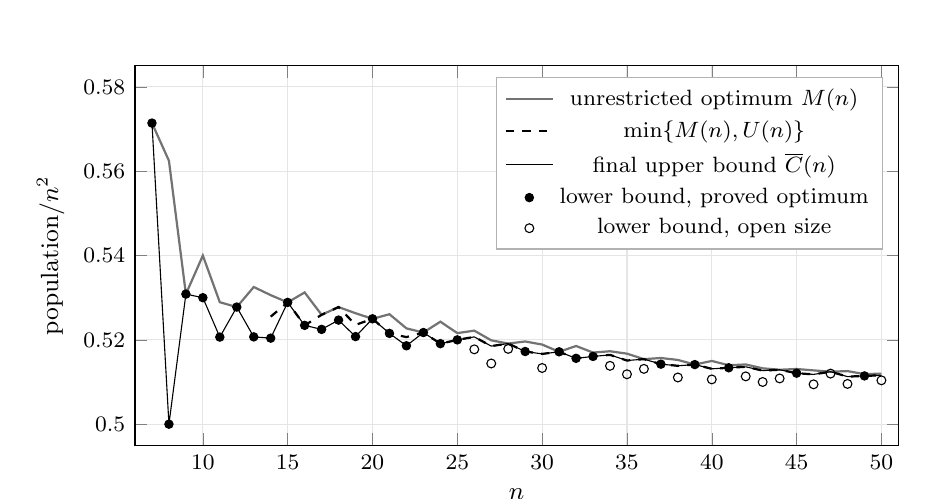
\begin{tikzpicture}
\begin{axis}[width=.93\textwidth,height=6.4cm,xlabel={$n$},ylabel={population$/n^2$},
 xmin=6,xmax=51,ymin=0.495,ymax=0.585,grid=both,grid style={black!10},
 legend style={font=\footnotesize,at={(0.98,0.97)},anchor=north east,draw=black!30},
 tick label style={font=\footnotesize},label style={font=\small}]
\addplot[black!55,thick,mark=none] coordinates {(7,0.57143) (8,0.56250) (9,0.53086) (10,0.54000) (11,0.52893) (12,0.52778) (13,0.53254) (14,0.53061) (15,0.52889) (16,0.53125) (17,0.52595) (18,0.52778) (19,0.52632) (20,0.52500) (21,0.52608) (22,0.52273) (23,0.52174) (24,0.52431) (25,0.52160) (26,0.52219) (27,0.51989) (28,0.51913) (29,0.51962) (30,0.51889) (31,0.51717) (32,0.51855) (33,0.51699) (34,0.51730) (35,0.51673) (36,0.51543) (37,0.51570) (38,0.51524) (39,0.51414) (40,0.51500) (41,0.51398) (42,0.51417) (43,0.51325) (44,0.51291) (45,0.51309) (46,0.51276) (47,0.51245) (48,0.51259) (49,0.51187) (50,0.51200)};
\addlegendentry{unrestricted optimum $M(n)$}
\addplot[black,thick,dashed,mark=none] coordinates {(14,0.52551) (15,0.52889) (16,0.52344) (17,0.52595) (18,0.52778) (19,0.52355) (20,0.52500) (21,0.52154) (22,0.52066) (23,0.52174) (24,0.51910) (25,0.52000) (26,0.52071) (27,0.51852) (28,0.51913) (29,0.51724) (30,0.51667) (31,0.51717) (32,0.51562) (33,0.51607) (34,0.51644) (35,0.51510) (36,0.51543) (37,0.51424) (38,0.51385) (39,0.51414) (40,0.51313) (41,0.51338) (42,0.51361) (43,0.51271) (44,0.51291) (45,0.51210) (46,0.51181) (47,0.51245) (48,0.51128) (49,0.51145) (50,0.51160)};
\addlegendentry{$\min\{M(n),U(n)\}$}
\addplot[black,thin,mark=none] coordinates {(7,0.57143) (8,0.50000) (9,0.53086) (10,0.53000) (11,0.52066) (12,0.52778) (13,0.52071) (14,0.52041) (15,0.52889) (16,0.52344) (17,0.52249) (18,0.52469) (19,0.52078) (20,0.52500) (21,0.52154) (22,0.51860) (23,0.52174) (24,0.51910) (25,0.52000) (26,0.52071) (27,0.51852) (28,0.51913) (29,0.51724) (30,0.51667) (31,0.51717) (32,0.51562) (33,0.51607) (34,0.51644) (35,0.51510) (36,0.51543) (37,0.51424) (38,0.51385) (39,0.51414) (40,0.51313) (41,0.51338) (42,0.51361) (43,0.51271) (44,0.51291) (45,0.51210) (46,0.51181) (47,0.51245) (48,0.51128) (49,0.51145) (50,0.51160)};
\addlegendentry{final upper bound $\overline C(n)$}
\addplot[only marks,mark=*,mark size=1.5pt,black] coordinates {(7,0.57143) (8,0.50000) (9,0.53086) (10,0.53000) (11,0.52066) (12,0.52778) (13,0.52071) (14,0.52041) (15,0.52889) (16,0.52344) (17,0.52249) (18,0.52469) (19,0.52078) (20,0.52500) (21,0.52154) (22,0.51860) (23,0.52174) (24,0.51910) (25,0.52000) (29,0.51724) (31,0.51717) (32,0.51562) (33,0.51607) (37,0.51424) (39,0.51414) (41,0.51338) (45,0.51210) (49,0.51145)};
\addlegendentry{lower bound, proved optimum}
\addplot[only marks,mark=o,mark size=1.6pt,black] coordinates {(26,0.51775) (27,0.51440) (28,0.51786) (30,0.51333) (34,0.51384) (35,0.51184) (36,0.51312) (38,0.51108) (40,0.51062) (42,0.51134) (43,0.51001) (44,0.51085) (46,0.50945) (47,0.51200) (48,0.50955) (50,0.51040)};
\addlegendentry{lower bound, open size}
\end{axis}
\end{tikzpicture}

\end{minipage}\hfill
\begin{minipage}{.49\textwidth}
\centering
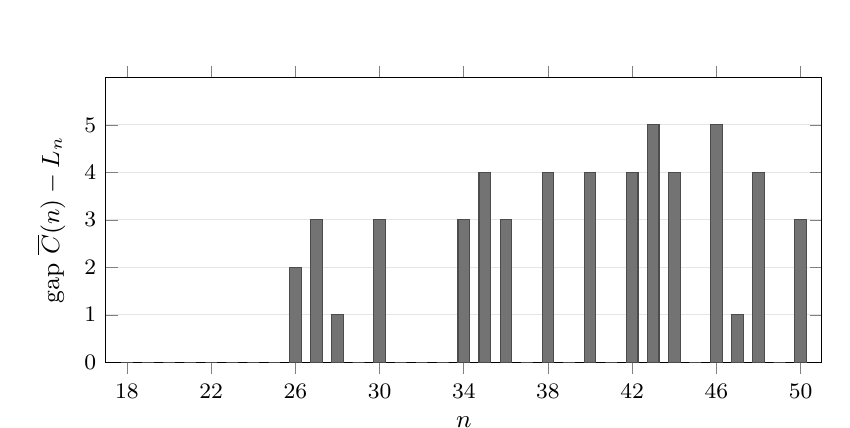
\begin{tikzpicture}
\begin{axis}[ybar,bar width=4.2pt,width=.88\textwidth,height=5.2cm,xlabel={$n$},
 ylabel={gap $\overline C(n)-L_n$},xmin=17,xmax=51,ymin=0,ymax=6,
 ytick={0,1,2,3,4,5},xtick={18,22,...,50},ymajorgrids=true,grid style={black!10},
 tick label style={font=\footnotesize},label style={font=\small}]
\addplot[fill=black!55,draw=black!70] coordinates {(18,0) (19,0) (20,0) (21,0) (22,0) (23,0) (24,0) (25,0) (26,2) (27,3) (28,1) (29,0) (30,3) (31,0) (32,0) (33,0) (34,3) (35,4) (36,3) (37,0) (38,4) (39,0) (40,4) (41,0) (42,4) (43,5) (44,4) (45,0) (46,5) (47,1) (48,4) (49,0) (50,3)};
\end{axis}
\end{tikzpicture}

\end{minipage}
\caption{Left: unrestricted optimum, connected upper bound, and verified lower
bound for $7\le n\le50$, normalized by area; filled markers are proved optima.
Densities can exceed $1/2$ because boundary cells receive the $O(n)$ edge bonus
of \eqref{eq:wastage}.  Right: the remaining gap $\overline C(n)-L_n$, at most
five, attained at $n=43$ and $n=46$.}
\label{fig:ledger}
\end{figure}

Small gaps do not by themselves indicate that a uniform formula is near.  At
$n=28$ and $n=47$ the intervals have width one, and in both cases
$M(n)=U(n)$, so a further cell needs either a connected board that is an
unrestricted optimum or an exclusion beyond the present boundary language.  The
construction-side difficulty is the compatibility of a dense periodic bulk with
four finite caps and one global component; the upper-bound difficulty is that a
shallow boundary relaxation need not detect a connectivity obstruction that
occurs only after several inward layers.

\section{Period-eight band families and a uniform lower bound}\label{sec:bands}

Let $S$ be a binary $n_0\times n_0$ seed and let $h\ge2$ satisfy $n_0-h-8\ge2$.
Call rows $h,\ldots,h+7$ and columns $h,\ldots,h+7$ of $S$ the \emph{bands}.  For
$k\ge1$ put $n=n_0+8(k-1)$ and
\begin{equation}\label{eq:band-index}
 f_k(i)=
 \begin{cases}
 i,&0\le i<h,\\
 h+((i-h)\bmod8),&h\le i<h+8k,\\
 i-8(k-1),&h+8k\le i<n,
 \end{cases}
 \qquad
 G_k(i,j)=S\bigl(f_k(i),f_k(j)\bigr).
\end{equation}
Thus $G_1=S$, and $G_{k+1}$ arises from $G_k$ by inserting one more copy of
each band.  The rows of $G_k$ fall into a top cap of $h$ rows, $k$ copies of the
band, and a bottom cap, and likewise the columns.  The resulting nine tile types
are four corners, four sides, and one centre, and the content of a tile depends
only on its type.  If $A$, $B$, $C$ count the live cells in the central tile, in
the four side tiles together, and in the four corner tiles together, then
\begin{equation}\label{eq:band-pop}
 |G_k|=Ak^2+Bk+C\qquad(k\ge1).
\end{equation}

Nine seeds were found by the search methods of \cref{app:repair}; they are
stored in \nolinkurl{ancillary/data/families.json}.  For each residue
$r\in\{0,\ldots,7\}$ there is a seed of side $24+r$, and a ninth seed of side
$40$ improves residue zero.  In every family the central $8\times8$ tile has
half density, $A=32$ (\cref{tab:bands}).

\begin{table}[t]
\centering
\caption{The nine band families: seed side $n_0$, band start $h$, tile counts
$A,B,C$ of \eqref{eq:band-pop}, deficit $a_r=n(n+1)/2-|G_k|$, and the radius $R$
of the connectivity certificate.  The primed row is the ninth family.}
\label{tab:bands}
\begin{tabular}{@{}ccccrrcc@{}}
\toprule
$r$ & $n_0$ & $h$ & $A$ & $B$ & $C$ & $a_r$ & $R$ \\
\midrule
0 & 24 & 8 & 32 & 132 & 132 & 4 & 2 \\
1 & 25 & 6 & 32 & 140 & 150 & 3 & 1 \\
2 & 26 & 8 & 32 & 148 & 167 & 4 & 2 \\
3 & 27 & 6 & 32 & 156 & 187 & 3 & 1 \\
4 & 28 & 6 & 32 & 164 & 206 & 4 & 1 \\
5 & 29 & 6 & 32 & 172 & 230 & 1 & 1 \\
6 & 30 & 6 & 32 & 180 & 250 & 3 & 1 \\
7 & 31 & 6 & 32 & 188 & 274 & 2 & 1 \\
0$'$ & 40 & 16 & 32 & 260 & 525 & 3 & 1 \\
\bottomrule
\end{tabular}

\end{table}

\begin{theorem}[Band families]\label{thm:bands}
Let $a=(a_0,\ldots,a_7)=(4,3,4,3,4,1,3,2)$.  For every $n\ge24$ there is a
connected still life in $\B_n$ of population
\begin{equation}\label{eq:band-family}
 \frac{n(n+1)}2-a_{n\bmod8},
\end{equation}
and for $n\equiv0\pmod8$, $n\ge40$, one of population $n(n+1)/2-3$.  Consequently
\begin{equation}\label{eq:uniform-lower}
 C(n)\ge\frac{n(n+1)}2-4\qquad\text{for every }n\ge1,
\end{equation}
and the constant $4$ is best possible.
\end{theorem}

Stability is local, but connectivity is not.  For each tile type list its
Moore components and, for every pair of neighbouring tile types (cardinal or
diagonal), the pairs of components joined across the common boundary.  In each
tile type call its largest component the \emph{main} component.  The tile grid
of $G_k$ has $k+2$ rows and columns, labelled top, band, \ldots, band, bottom.
For $R\ge1$, the \emph{context} of a tile position is the array of labels of the
tiles within distance $R$ in each coordinate, clipped at the boundary.  A family
is \emph{$R$-linked} if, for every $k\in\{1,\ldots,2R+1\}$ and every tile
position of $G_k$, inside the graph spanned by the tiles of its context, every
component of the tile and the main component of each cardinally adjacent tile
are joined to the main component of the tile.

\begin{lemma}[Connectivity pumping]\label{lem:pumping}
If a band family is $R$-linked, then $G_k$ is connected for every $k\ge1$.
\end{lemma}

\begin{proof}
In one direction the clipped context at tile index $p\in\{0,\ldots,k+1\}$ is
determined by $(\min(p,R),\min(k+1-p,R))$.  For $k\ge2R+1$ the set of these
pairs is $\{(p,R):p\le R\}\cup\{(R,R)\}\cup\{(R,q):q\le R\}$, independent of $k$
and already realized at $k=2R+1$.  A context in the plane is a pair of a row and
a column context, and tile contents and interfaces depend only on tile types, so
the linking property holds at every position of every $G_k$.  Hence every
component is joined to the main component of its tile, the main components of
cardinally adjacent tiles are joined, and since the tile grid is connected, so
is $G_k$.
\end{proof}

\begin{proof}[Proof of \cref{thm:bands}]
\emph{Population.}  For each seed, \cref{tab:bands} gives $A=32$, and
substituting $k=(n-n_0)/8+1$ into \eqref{eq:band-pop} gives exactly
$n(n+1)/2-a_r$.  For instance, for $r=5$ and $n=21+8k$ one has
$n(n+1)/2=32k^2+172k+231$ and $|G_k|=32k^2+172k+230$.  Both sides are
quadratics in $k$ with leading coefficient $32$, so comparing the other two
coefficients suffices.  The ninth family has $|G_k|=32k^2+260k+525=n(n+1)/2-3$
with $n=32+8k$.

\emph{Stability.}  Stability is a condition on the $3\times3$ windows of the
zero-extended array at the centres of $\B_n\cup R_n$.  The caps and the band
each have at least two lines, so three consecutive lines of $G_k$ are three
consecutive lines of $S$, or straddle a seam between two band copies (lines
$h+6,h+7,h$ or $h+7,h,h+1$), possibly with dead lines beyond the boundary.  The
set of such types is the same for all $k\ge2$, and a window is a pair of a row
type and a column type, so every window of $G_k$ with $k\ge3$ occurs in $G_2$.
Direct verification of $G_1$ and $G_2$ on $\B_n\cup R_n$ therefore proves
stability for all $k$.

\emph{Connectivity.}  The base families with $r=0$ and $r=2$ are $2$-linked,
with 79 distinct contexts, and the other seven are $1$-linked, with 30.
\Cref{lem:pumping} gives connectivity for every $k$.

\emph{The uniform bound.}  Every $n\ge24$ equals $n_0+8(k-1)$ for the seed with
$n_0=24+(n\bmod8)$ and some $k\ge1$, and the largest deficit is $4$.  For
$n\le23$ the exact values give $C(n)-n(n+1)/2\ge-4$:
\[
\scriptsize
\begin{array}{c|ccccccccccccccccccccccc}
n&1&2&3&4&5&6&7&8&9&10&11&12&13&14&15&16&17&18&19&20&21&22&23\\
\hline
C(n)-\frac{n(n+1)}2&-1&1&0&-2&-4&-3&0&-4&-2&-2&-3&-2&-3&-3&-1&-2&-2&-1&-2&0&-1&-2&0
\end{array}
\]
Equality occurs at $n=5$ and $n=8$, so the constant $4$ is best possible.  The
population formulas, the window containment for $3\le k\le8$, every context, and
the absence of new contexts for $2R+1\le k\le2R+4$ are rechecked by the audit
script of \cref{app:certificates}.
\end{proof}

\begin{figure}[t]
\centering
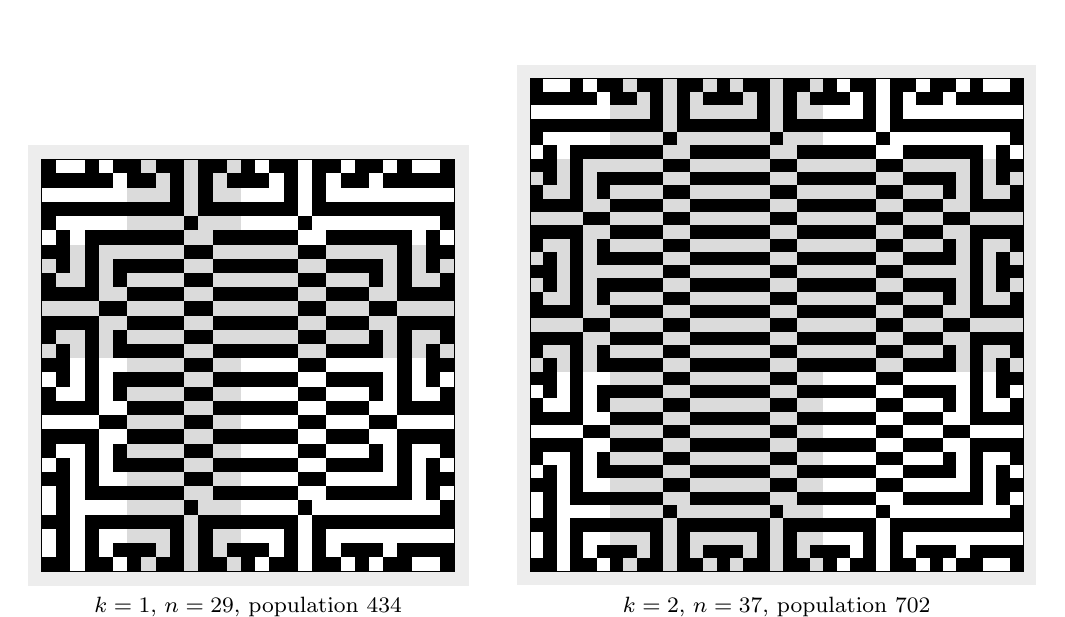
\begin{tikzpicture}
\begin{scope}[xshift=0.000cm]
\begin{scope}[x=0.1806cm,y=0.1806cm]
\fill[black!7] (-1,-1) rectangle (30,30);
\fill[white] (0,0) rectangle (29,29);
\fill[black!14] (0,15) rectangle (29,23);
\fill[black!14] (6,0) rectangle (14,29);
\draw[black,line width=.35pt] (0,0) rectangle (29,29);
\fill (0,28) rectangle (1,29);
\fill (3,28) rectangle (4,29);
\fill (5,28) rectangle (7,29);
\fill (8,28) rectangle (10,29);
\fill (11,28) rectangle (13,29);
\fill (14,28) rectangle (15,29);
\fill (16,28) rectangle (18,29);
\fill (19,28) rectangle (21,29);
\fill (22,28) rectangle (24,29);
\fill (25,28) rectangle (26,29);
\fill (28,28) rectangle (29,29);
\fill (0,27) rectangle (5,28);
\fill (6,27) rectangle (8,28);
\fill (9,27) rectangle (10,28);
\fill (11,27) rectangle (12,28);
\fill (13,27) rectangle (16,28);
\fill (17,27) rectangle (18,28);
\fill (19,27) rectangle (20,28);
\fill (21,27) rectangle (23,28);
\fill (24,27) rectangle (29,28);
\fill (9,26) rectangle (10,27);
\fill (11,26) rectangle (12,27);
\fill (17,26) rectangle (18,27);
\fill (19,26) rectangle (20,27);
\fill (0,25) rectangle (10,26);
\fill (11,25) rectangle (18,26);
\fill (19,25) rectangle (29,26);
\fill (0,24) rectangle (1,25);
\fill (10,24) rectangle (11,25);
\fill (18,24) rectangle (19,25);
\fill (28,24) rectangle (29,25);
\fill (1,23) rectangle (2,24);
\fill (3,23) rectangle (10,24);
\fill (12,23) rectangle (18,24);
\fill (20,23) rectangle (26,24);
\fill (27,23) rectangle (28,24);
\fill (0,22) rectangle (2,23);
\fill (3,22) rectangle (4,23);
\fill (10,22) rectangle (12,23);
\fill (18,22) rectangle (20,23);
\fill (25,22) rectangle (26,23);
\fill (27,22) rectangle (29,23);
\fill (1,21) rectangle (2,22);
\fill (3,21) rectangle (4,22);
\fill (5,21) rectangle (10,22);
\fill (12,21) rectangle (18,22);
\fill (20,21) rectangle (24,22);
\fill (25,21) rectangle (26,22);
\fill (27,21) rectangle (28,22);
\fill (0,20) rectangle (1,21);
\fill (3,20) rectangle (4,21);
\fill (5,20) rectangle (6,21);
\fill (10,20) rectangle (12,21);
\fill (18,20) rectangle (20,21);
\fill (23,20) rectangle (24,21);
\fill (25,20) rectangle (26,21);
\fill (28,20) rectangle (29,21);
\fill (0,19) rectangle (4,20);
\fill (6,19) rectangle (10,20);
\fill (12,19) rectangle (18,20);
\fill (20,19) rectangle (23,20);
\fill (25,19) rectangle (29,20);
\fill (4,18) rectangle (6,19);
\fill (10,18) rectangle (12,19);
\fill (18,18) rectangle (20,19);
\fill (23,18) rectangle (25,19);
\fill (0,17) rectangle (4,18);
\fill (6,17) rectangle (10,18);
\fill (12,17) rectangle (18,18);
\fill (20,17) rectangle (23,18);
\fill (25,17) rectangle (29,18);
\fill (0,16) rectangle (1,17);
\fill (3,16) rectangle (4,17);
\fill (5,16) rectangle (6,17);
\fill (10,16) rectangle (12,17);
\fill (18,16) rectangle (20,17);
\fill (23,16) rectangle (24,17);
\fill (25,16) rectangle (26,17);
\fill (28,16) rectangle (29,17);
\fill (1,15) rectangle (2,16);
\fill (3,15) rectangle (4,16);
\fill (5,15) rectangle (10,16);
\fill (12,15) rectangle (18,16);
\fill (20,15) rectangle (24,16);
\fill (25,15) rectangle (26,16);
\fill (27,15) rectangle (28,16);
\fill (0,14) rectangle (2,15);
\fill (3,14) rectangle (4,15);
\fill (10,14) rectangle (12,15);
\fill (18,14) rectangle (20,15);
\fill (25,14) rectangle (26,15);
\fill (27,14) rectangle (29,15);
\fill (1,13) rectangle (2,14);
\fill (3,13) rectangle (4,14);
\fill (5,13) rectangle (10,14);
\fill (12,13) rectangle (18,14);
\fill (20,13) rectangle (24,14);
\fill (25,13) rectangle (26,14);
\fill (27,13) rectangle (28,14);
\fill (0,12) rectangle (1,13);
\fill (3,12) rectangle (4,13);
\fill (5,12) rectangle (6,13);
\fill (10,12) rectangle (12,13);
\fill (18,12) rectangle (20,13);
\fill (23,12) rectangle (24,13);
\fill (25,12) rectangle (26,13);
\fill (28,12) rectangle (29,13);
\fill (0,11) rectangle (4,12);
\fill (6,11) rectangle (10,12);
\fill (12,11) rectangle (18,12);
\fill (20,11) rectangle (23,12);
\fill (25,11) rectangle (29,12);
\fill (4,10) rectangle (6,11);
\fill (10,10) rectangle (12,11);
\fill (18,10) rectangle (20,11);
\fill (23,10) rectangle (25,11);
\fill (0,9) rectangle (4,10);
\fill (6,9) rectangle (10,10);
\fill (12,9) rectangle (18,10);
\fill (20,9) rectangle (23,10);
\fill (25,9) rectangle (29,10);
\fill (0,8) rectangle (1,9);
\fill (3,8) rectangle (4,9);
\fill (5,8) rectangle (6,9);
\fill (10,8) rectangle (12,9);
\fill (18,8) rectangle (20,9);
\fill (23,8) rectangle (24,9);
\fill (25,8) rectangle (26,9);
\fill (28,8) rectangle (29,9);
\fill (1,7) rectangle (2,8);
\fill (3,7) rectangle (4,8);
\fill (5,7) rectangle (10,8);
\fill (12,7) rectangle (18,8);
\fill (20,7) rectangle (24,8);
\fill (25,7) rectangle (26,8);
\fill (27,7) rectangle (28,8);
\fill (0,6) rectangle (2,7);
\fill (3,6) rectangle (4,7);
\fill (10,6) rectangle (12,7);
\fill (18,6) rectangle (20,7);
\fill (25,6) rectangle (26,7);
\fill (27,6) rectangle (29,7);
\fill (1,5) rectangle (2,6);
\fill (3,5) rectangle (10,6);
\fill (12,5) rectangle (18,6);
\fill (20,5) rectangle (26,6);
\fill (27,5) rectangle (28,6);
\fill (1,4) rectangle (2,5);
\fill (10,4) rectangle (11,5);
\fill (18,4) rectangle (19,5);
\fill (28,4) rectangle (29,5);
\fill (0,3) rectangle (2,4);
\fill (3,3) rectangle (10,4);
\fill (11,3) rectangle (18,4);
\fill (19,3) rectangle (29,4);
\fill (1,2) rectangle (2,3);
\fill (3,2) rectangle (4,3);
\fill (9,2) rectangle (10,3);
\fill (11,2) rectangle (12,3);
\fill (17,2) rectangle (18,3);
\fill (19,2) rectangle (20,3);
\fill (1,1) rectangle (2,2);
\fill (3,1) rectangle (4,2);
\fill (5,1) rectangle (8,2);
\fill (9,1) rectangle (10,2);
\fill (11,1) rectangle (12,2);
\fill (13,1) rectangle (16,2);
\fill (17,1) rectangle (18,2);
\fill (19,1) rectangle (20,2);
\fill (21,1) rectangle (24,2);
\fill (25,1) rectangle (29,2);
\fill (0,0) rectangle (2,1);
\fill (3,0) rectangle (5,1);
\fill (6,0) rectangle (7,1);
\fill (8,0) rectangle (10,1);
\fill (11,0) rectangle (13,1);
\fill (14,0) rectangle (15,1);
\fill (16,0) rectangle (18,1);
\fill (19,0) rectangle (21,1);
\fill (22,0) rectangle (23,1);
\fill (24,0) rectangle (26,1);
\fill (28,0) rectangle (29,1);
\end{scope}
\node[font=\footnotesize] at (2.619,-0.45) {$k=1$, $n=29$, population $434$};
\end{scope}
\begin{scope}[xshift=6.200cm]
\begin{scope}[x=0.1692cm,y=0.1692cm]
\fill[black!7] (-1,-1) rectangle (38,38);
\fill[white] (0,0) rectangle (37,37);
\fill[black!14] (0,15) rectangle (37,31);
\fill[black!14] (6,0) rectangle (22,37);
\draw[black,line width=.35pt] (0,0) rectangle (37,37);
\fill (0,36) rectangle (1,37);
\fill (3,36) rectangle (4,37);
\fill (5,36) rectangle (7,37);
\fill (8,36) rectangle (10,37);
\fill (11,36) rectangle (13,37);
\fill (14,36) rectangle (15,37);
\fill (16,36) rectangle (18,37);
\fill (19,36) rectangle (21,37);
\fill (22,36) rectangle (23,37);
\fill (24,36) rectangle (26,37);
\fill (27,36) rectangle (29,37);
\fill (30,36) rectangle (32,37);
\fill (33,36) rectangle (34,37);
\fill (36,36) rectangle (37,37);
\fill (0,35) rectangle (5,36);
\fill (6,35) rectangle (8,36);
\fill (9,35) rectangle (10,36);
\fill (11,35) rectangle (12,36);
\fill (13,35) rectangle (16,36);
\fill (17,35) rectangle (18,36);
\fill (19,35) rectangle (20,36);
\fill (21,35) rectangle (24,36);
\fill (25,35) rectangle (26,36);
\fill (27,35) rectangle (28,36);
\fill (29,35) rectangle (31,36);
\fill (32,35) rectangle (37,36);
\fill (9,34) rectangle (10,35);
\fill (11,34) rectangle (12,35);
\fill (17,34) rectangle (18,35);
\fill (19,34) rectangle (20,35);
\fill (25,34) rectangle (26,35);
\fill (27,34) rectangle (28,35);
\fill (0,33) rectangle (10,34);
\fill (11,33) rectangle (18,34);
\fill (19,33) rectangle (26,34);
\fill (27,33) rectangle (37,34);
\fill (0,32) rectangle (1,33);
\fill (10,32) rectangle (11,33);
\fill (18,32) rectangle (19,33);
\fill (26,32) rectangle (27,33);
\fill (36,32) rectangle (37,33);
\fill (1,31) rectangle (2,32);
\fill (3,31) rectangle (10,32);
\fill (12,31) rectangle (18,32);
\fill (20,31) rectangle (26,32);
\fill (28,31) rectangle (34,32);
\fill (35,31) rectangle (36,32);
\fill (0,30) rectangle (2,31);
\fill (3,30) rectangle (4,31);
\fill (10,30) rectangle (12,31);
\fill (18,30) rectangle (20,31);
\fill (26,30) rectangle (28,31);
\fill (33,30) rectangle (34,31);
\fill (35,30) rectangle (37,31);
\fill (1,29) rectangle (2,30);
\fill (3,29) rectangle (4,30);
\fill (5,29) rectangle (10,30);
\fill (12,29) rectangle (18,30);
\fill (20,29) rectangle (26,30);
\fill (28,29) rectangle (32,30);
\fill (33,29) rectangle (34,30);
\fill (35,29) rectangle (36,30);
\fill (0,28) rectangle (1,29);
\fill (3,28) rectangle (4,29);
\fill (5,28) rectangle (6,29);
\fill (10,28) rectangle (12,29);
\fill (18,28) rectangle (20,29);
\fill (26,28) rectangle (28,29);
\fill (31,28) rectangle (32,29);
\fill (33,28) rectangle (34,29);
\fill (36,28) rectangle (37,29);
\fill (0,27) rectangle (4,28);
\fill (6,27) rectangle (10,28);
\fill (12,27) rectangle (18,28);
\fill (20,27) rectangle (26,28);
\fill (28,27) rectangle (31,28);
\fill (33,27) rectangle (37,28);
\fill (4,26) rectangle (6,27);
\fill (10,26) rectangle (12,27);
\fill (18,26) rectangle (20,27);
\fill (26,26) rectangle (28,27);
\fill (31,26) rectangle (33,27);
\fill (0,25) rectangle (4,26);
\fill (6,25) rectangle (10,26);
\fill (12,25) rectangle (18,26);
\fill (20,25) rectangle (26,26);
\fill (28,25) rectangle (31,26);
\fill (33,25) rectangle (37,26);
\fill (0,24) rectangle (1,25);
\fill (3,24) rectangle (4,25);
\fill (5,24) rectangle (6,25);
\fill (10,24) rectangle (12,25);
\fill (18,24) rectangle (20,25);
\fill (26,24) rectangle (28,25);
\fill (31,24) rectangle (32,25);
\fill (33,24) rectangle (34,25);
\fill (36,24) rectangle (37,25);
\fill (1,23) rectangle (2,24);
\fill (3,23) rectangle (4,24);
\fill (5,23) rectangle (10,24);
\fill (12,23) rectangle (18,24);
\fill (20,23) rectangle (26,24);
\fill (28,23) rectangle (32,24);
\fill (33,23) rectangle (34,24);
\fill (35,23) rectangle (36,24);
\fill (0,22) rectangle (2,23);
\fill (3,22) rectangle (4,23);
\fill (10,22) rectangle (12,23);
\fill (18,22) rectangle (20,23);
\fill (26,22) rectangle (28,23);
\fill (33,22) rectangle (34,23);
\fill (35,22) rectangle (37,23);
\fill (1,21) rectangle (2,22);
\fill (3,21) rectangle (4,22);
\fill (5,21) rectangle (10,22);
\fill (12,21) rectangle (18,22);
\fill (20,21) rectangle (26,22);
\fill (28,21) rectangle (32,22);
\fill (33,21) rectangle (34,22);
\fill (35,21) rectangle (36,22);
\fill (0,20) rectangle (1,21);
\fill (3,20) rectangle (4,21);
\fill (5,20) rectangle (6,21);
\fill (10,20) rectangle (12,21);
\fill (18,20) rectangle (20,21);
\fill (26,20) rectangle (28,21);
\fill (31,20) rectangle (32,21);
\fill (33,20) rectangle (34,21);
\fill (36,20) rectangle (37,21);
\fill (0,19) rectangle (4,20);
\fill (6,19) rectangle (10,20);
\fill (12,19) rectangle (18,20);
\fill (20,19) rectangle (26,20);
\fill (28,19) rectangle (31,20);
\fill (33,19) rectangle (37,20);
\fill (4,18) rectangle (6,19);
\fill (10,18) rectangle (12,19);
\fill (18,18) rectangle (20,19);
\fill (26,18) rectangle (28,19);
\fill (31,18) rectangle (33,19);
\fill (0,17) rectangle (4,18);
\fill (6,17) rectangle (10,18);
\fill (12,17) rectangle (18,18);
\fill (20,17) rectangle (26,18);
\fill (28,17) rectangle (31,18);
\fill (33,17) rectangle (37,18);
\fill (0,16) rectangle (1,17);
\fill (3,16) rectangle (4,17);
\fill (5,16) rectangle (6,17);
\fill (10,16) rectangle (12,17);
\fill (18,16) rectangle (20,17);
\fill (26,16) rectangle (28,17);
\fill (31,16) rectangle (32,17);
\fill (33,16) rectangle (34,17);
\fill (36,16) rectangle (37,17);
\fill (1,15) rectangle (2,16);
\fill (3,15) rectangle (4,16);
\fill (5,15) rectangle (10,16);
\fill (12,15) rectangle (18,16);
\fill (20,15) rectangle (26,16);
\fill (28,15) rectangle (32,16);
\fill (33,15) rectangle (34,16);
\fill (35,15) rectangle (36,16);
\fill (0,14) rectangle (2,15);
\fill (3,14) rectangle (4,15);
\fill (10,14) rectangle (12,15);
\fill (18,14) rectangle (20,15);
\fill (26,14) rectangle (28,15);
\fill (33,14) rectangle (34,15);
\fill (35,14) rectangle (37,15);
\fill (1,13) rectangle (2,14);
\fill (3,13) rectangle (4,14);
\fill (5,13) rectangle (10,14);
\fill (12,13) rectangle (18,14);
\fill (20,13) rectangle (26,14);
\fill (28,13) rectangle (32,14);
\fill (33,13) rectangle (34,14);
\fill (35,13) rectangle (36,14);
\fill (0,12) rectangle (1,13);
\fill (3,12) rectangle (4,13);
\fill (5,12) rectangle (6,13);
\fill (10,12) rectangle (12,13);
\fill (18,12) rectangle (20,13);
\fill (26,12) rectangle (28,13);
\fill (31,12) rectangle (32,13);
\fill (33,12) rectangle (34,13);
\fill (36,12) rectangle (37,13);
\fill (0,11) rectangle (4,12);
\fill (6,11) rectangle (10,12);
\fill (12,11) rectangle (18,12);
\fill (20,11) rectangle (26,12);
\fill (28,11) rectangle (31,12);
\fill (33,11) rectangle (37,12);
\fill (4,10) rectangle (6,11);
\fill (10,10) rectangle (12,11);
\fill (18,10) rectangle (20,11);
\fill (26,10) rectangle (28,11);
\fill (31,10) rectangle (33,11);
\fill (0,9) rectangle (4,10);
\fill (6,9) rectangle (10,10);
\fill (12,9) rectangle (18,10);
\fill (20,9) rectangle (26,10);
\fill (28,9) rectangle (31,10);
\fill (33,9) rectangle (37,10);
\fill (0,8) rectangle (1,9);
\fill (3,8) rectangle (4,9);
\fill (5,8) rectangle (6,9);
\fill (10,8) rectangle (12,9);
\fill (18,8) rectangle (20,9);
\fill (26,8) rectangle (28,9);
\fill (31,8) rectangle (32,9);
\fill (33,8) rectangle (34,9);
\fill (36,8) rectangle (37,9);
\fill (1,7) rectangle (2,8);
\fill (3,7) rectangle (4,8);
\fill (5,7) rectangle (10,8);
\fill (12,7) rectangle (18,8);
\fill (20,7) rectangle (26,8);
\fill (28,7) rectangle (32,8);
\fill (33,7) rectangle (34,8);
\fill (35,7) rectangle (36,8);
\fill (0,6) rectangle (2,7);
\fill (3,6) rectangle (4,7);
\fill (10,6) rectangle (12,7);
\fill (18,6) rectangle (20,7);
\fill (26,6) rectangle (28,7);
\fill (33,6) rectangle (34,7);
\fill (35,6) rectangle (37,7);
\fill (1,5) rectangle (2,6);
\fill (3,5) rectangle (10,6);
\fill (12,5) rectangle (18,6);
\fill (20,5) rectangle (26,6);
\fill (28,5) rectangle (34,6);
\fill (35,5) rectangle (36,6);
\fill (1,4) rectangle (2,5);
\fill (10,4) rectangle (11,5);
\fill (18,4) rectangle (19,5);
\fill (26,4) rectangle (27,5);
\fill (36,4) rectangle (37,5);
\fill (0,3) rectangle (2,4);
\fill (3,3) rectangle (10,4);
\fill (11,3) rectangle (18,4);
\fill (19,3) rectangle (26,4);
\fill (27,3) rectangle (37,4);
\fill (1,2) rectangle (2,3);
\fill (3,2) rectangle (4,3);
\fill (9,2) rectangle (10,3);
\fill (11,2) rectangle (12,3);
\fill (17,2) rectangle (18,3);
\fill (19,2) rectangle (20,3);
\fill (25,2) rectangle (26,3);
\fill (27,2) rectangle (28,3);
\fill (1,1) rectangle (2,2);
\fill (3,1) rectangle (4,2);
\fill (5,1) rectangle (8,2);
\fill (9,1) rectangle (10,2);
\fill (11,1) rectangle (12,2);
\fill (13,1) rectangle (16,2);
\fill (17,1) rectangle (18,2);
\fill (19,1) rectangle (20,2);
\fill (21,1) rectangle (24,2);
\fill (25,1) rectangle (26,2);
\fill (27,1) rectangle (28,2);
\fill (29,1) rectangle (32,2);
\fill (33,1) rectangle (37,2);
\fill (0,0) rectangle (2,1);
\fill (3,0) rectangle (5,1);
\fill (6,0) rectangle (7,1);
\fill (8,0) rectangle (10,1);
\fill (11,0) rectangle (13,1);
\fill (14,0) rectangle (15,1);
\fill (16,0) rectangle (18,1);
\fill (19,0) rectangle (21,1);
\fill (22,0) rectangle (23,1);
\fill (24,0) rectangle (26,1);
\fill (27,0) rectangle (29,1);
\fill (30,0) rectangle (31,1);
\fill (32,0) rectangle (34,1);
\fill (36,0) rectangle (37,1);
\end{scope}
\node[font=\footnotesize] at (3.131,-0.45) {$k=2$, $n=37$, population $702$};
\end{scope}
\end{tikzpicture}

\caption{The band family of residue $r=5$ at $k=1$ (the seed, $n_0=29$) and
$k=2$ ($n=37$).  Shaded rows and columns are the repeated bands.}
\label{fig:band-family}
\end{figure}

\begin{theorem}[Density]\label{thm:density}
$\lim_{n\to\infty}C(n)/n^2=1/2$.  More precisely,
\[
 \frac12\le\liminf_{n\to\infty}\frac{C(n)-n^2/2}n\le
 \limsup_{n\to\infty}\frac{C(n)-n^2/2}n\le\frac58.
\]
\end{theorem}

\begin{proof}
The lower bounds follow from \cref{thm:bands}, since $C(n)\ge n^2/2+n/2-4$.  The
upper bounds follow from $C(n)\le U(n)\le n^2/2+5n/8$.
\end{proof}

The earlier families of \cref{app:families} are weaker: the pond lattice has
density $4/9$, the capped bricks have density $1/2$ with a negative linear
coefficient, and the period-fifty-four family has linear coefficient $13/27<1/2$.
The bound \eqref{eq:uniform-lower} is not an upper bound either:
$C(65)=2150=65\cdot66/2+5$.  Whether $C(n)-n(n+1)/2$ is bounded is open.  The
density statement is consistent with Elkies's theorem for infinite still
lifes~\cite{elkies-1999}.

\section{Open questions}\label{sec:open}

The immediate finite problems are $350\le C(26)\le352$ and the one-cell
intervals $406\le C(28)\le407$ and $1131\le C(47)\le1132$.

The chains of \cref{sec:closures-U} suggest a sharper question: is
$C(n)=U(n)$ for every $n\equiv5\pmod8$ with $n\ge21$ and every $n\equiv1\pmod8$
with $n\ge25$?  In the other classes the optimum equals $U(n)$ at $n=16,24,32$
and is strictly smaller at $n=14,17,18,19,22$.

The upper expression satisfies the exact period of \cref{cor:U-recurrence}, but
that is not a recurrence for $C(n)$: a construction pump must carry compatible
states through all four corners, fill the enlarged interior stably, and preserve
one component.  The band families achieve this with linear coefficient $1/2$,
while $U$ has linear coefficient $5/8$, and the true linear coefficient is not
known.  A natural route to an exact formula is a pair of finite transducers whose
states record the four boundary phases together with a connectivity signature of
the interior interface; the present boundary automata control wastage but forget
that global information.

The sequence $C(n)$ appears in the On-Line Encyclopedia of Integer Sequences as
A398723~\cite{oeis-a398723}, with the unrestricted sequence A055397 as its
companion upper bound~\cite{oeis-a055397}.  All boards, certificates, scripts,
and verifiers are available in the public repository~\cite{repo}.

\section*{Acknowledgments}

The author thanks Paras Chopra, his mentor at Lossfunk, for guidance and support
throughout this work.  Dr.~Ankan Pal (Birla Institute of Technology and
Science, Pilani) served as reviewer of the Connected Still Life problem in the
CAISc 2026 Verifiable Problems Track, and the author thanks him for his review.
The author thanks the CAISc 2026 organizing team, Dhruv Trehan, Dhruv Kumar,
Sasank Tripathi, and Devansh Agarwal, who organized the track from which the
problem was drawn and who were co-authors of an earlier version of this
manuscript, and the authors of the accepted CAISc submissions, whose boards and
methods informed this work.

\subsection*{AI declaration}

OpenAI's ChatGPT (Sol 5.6 and 6 Astra) was used mainly to find and run the
search programs, certificate generators, and proofs, and Anthropic's Claude was
used to help prepare this manuscript.  The author directed the work, checked the
claims, and is responsible for every statement.  Every result rests on a
verified board, a finite certificate, a cited theorem, or an argument given in
the paper.

\begingroup
\footnotesize
\begin{thebibliography}{99}

\bibitem{elkies-1999}
N. D. Elkies,
The still-life density problem and its generalizations,
\emph{Voronoi's Impact on Modern Science}, Book I, 228--253, 1998;
arXiv:math/9905194.

\bibitem{larrosa-2005}
J. Larrosa, E. Morancho, and D. Niso,
On the practical use of variable elimination in constraint optimization
problems: ``still-life'' as a case study,
\emph{Journal of Artificial Intelligence Research} 23 (2005), 421--440.

\bibitem{chu-stuckey-garcia-2009}
G. Chu, P. J. Stuckey, and M. Garcia de la Banda,
Using relaxations in maximum density still life,
in \emph{Principles and Practice of Constraint Programming},
Lecture Notes in Computer Science 5732, Springer, 2009, 258--273.

\bibitem{chu-stuckey-2012}
G. Chu and P. J. Stuckey,
A complete solution to the maximum density still life problem,
\emph{Artificial Intelligence} 184--185 (2012), 1--16.

\bibitem{drescher-2013}
Connected maximum-density still life, benchmark of the Fourth Answer Set
Programming Competition, 2013,
\url{https://www.mat.unical.it/aspcomp2013/ConnectedMaximumDensityStillLife}.

\bibitem{oeis-a055397}
OEIS Foundation,
A055397: maximum number of live cells in a still life of Conway's Game of Life
fitting in an $n\times n$ square,
\url{https://oeis.org/A055397}.

\bibitem{oeis-a398723}
OEIS Foundation,
A398723: maximum population of an 8-connected still life contained in an
$n\times n$ square in Conway's Game of Life, with a dead exterior,
\url{https://oeis.org/A398723}.

\bibitem{repo}
S. Mahajan,
Maximum connected still lifes: witnesses, bounds, and reproducible optimality
proofs, \url{https://github.com/Siddhartha-Mahajan/connected-still-life}, 2026.

\bibitem{caisc-problem}
S. Mahajan,
Connected Still Life, CAISc 2026 Verifiable Problems Track, 2026,
\url{https://caisc2026.github.io/verifiable-problems/?problem=connected-still-life}.

\bibitem{caisc-collier}
M. Collier and B. Derfer,
Connected Still Life Across an AI-Inclusive Cognitive Ecosystem: A
Verifier-Attested Case Study, CAISc 2026,
\url{https://openreview.net/forum?id=2RLaZFD49N}.

\bibitem{caisc-jaswal}
A. S. Jaswal,
How Dense Can a Connected Still Life Be? Records, Proven Optima, and
Machine-Checked Certificates up to $n=32$, CAISc 2026,
\url{https://openreview.net/forum?id=3WPIRgk9pS}.

\bibitem{caisc-menta}
V. P. T. Menta,
Verifier-Clean Connected Still Lifes Across All Box Sizes: A Complete CP-SAT
Encoding with Annealing Polish, CAISc 2026,
\url{https://openreview.net/forum?id=4LBYPzoSUW}.

\bibitem{caisc-reddy}
S. Reddy, J. M. S. Zakkam, S. R. Kanakamedala, S. Myana, and S. S. Gunturi,
Still Life, Still Living: An LLM Coding Agent's Trajectory on Connected
Game-of-Life Patterns, CAISc 2026,
\url{https://openreview.net/forum?id=ojLUNf0fcA}.

\bibitem{caisc-rushdi}
A. A. Rushdi,
A Spanning-Tree Encoding for the Connected Maximum Still-Life Problem, CAISc
2026, \url{https://openreview.net/forum?id=c14oLVAvr5}.

\bibitem{caisc-sodha}
T. Sodha,
The Cost of Connectivity: Exact and Heuristic Bounds for the Connected Maximum
Density Still Life Problem, CAISc 2026,
\url{https://openreview.net/forum?id=l3mTljsAht}.

\bibitem{caisc-sridhar}
P. Sridhar,
Hybrid Exact and Heuristic Search for Dense Connected Still Lifes, CAISc 2026,
\url{https://openreview.net/forum?id=BGHqGZz1iK}.

\end{thebibliography}
\endgroup

\appendix

\section{The CAISc 2026 challenge}\label{app:caisc}

The first Conference for AI Scientists (CAISc 2026) was held online on 24--25
July 2026; its Verifiable Problems Track paired each submission with an
automatically checkable artifact~\cite{caisc-problem}.  For a prescribed size
$n$, an artifact was a binary array $x\in\{0,1\}^{n\times n}$ and a claimed
population $p$, accepted exactly when $p=\sum x_{ij}$, the B3/S23 conditions
held on the board and its complete dead ring, and the support was one Moore
component.  An accepted artifact therefore proves $C(n)\ge p$ but says nothing
about $C(n)\le p$.  \Cref{tab:caisc-submissions} summarizes the seven accepted
submissions; the entries report their own claims.

\begin{table}[h]
\centering
\caption{Accepted CAISc 2026 connected-still-life submissions.}
\label{tab:caisc-submissions}
\scriptsize
\begin{tabularx}{\textwidth}{@{}>{\raggedright\arraybackslash}p{0.11\textwidth}>{\raggedright\arraybackslash}p{0.33\textwidth}X@{}}
\toprule
submission & stated results & principal methods\\
\midrule
Collier~\cite{caisc-collier} & exact for $n\in\{8,9,10,11,13\}$; $209,495,526$ at $n=20,31,32$ & wastage-aware CP-SAT with lazy connectivity, MaxSAT, Chuffed, an IPASIR-UP propagator, stripe DP, cross-engine validation\\
Jaswal~\cite{caisc-jaswal} & exact for $n\in\{8,9,10,11,15\}$; $133,208,495,524$ at $n=16,20,31,32$ & pseudo-Boolean model with strict-rank connectivity and VeriPB proof logging, CP-SAT, large-neighbourhood search; the $2\times8$ brick motif\\
Menta~\cite{caisc-menta} & exact for $n\in\{8,9,10\}$; $133,207,485,515$ at $n=16,20,31,32$ & complete CP-SAT with breadth-first connectivity, symmetry, parallel tempering, verifier-gated acceptance\\
Reddy~\cite{caisc-reddy} & exact for $n\in\{8,9,15\}$; $133,207,495,525$ at $n=16,20,31,32$ & CP-SAT, strip DP, symmetry audits, exact re-solving of pockets cut from dense still lifes\\
Rushdi~\cite{caisc-rushdi} & exact for $n\in\{8,9,10,11,15\}$; $132,206,479,515$ at $n=16,20,31,32$ & parent-pointer spanning tree in CP-SAT, local-search polishing\\
Sodha~\cite{caisc-sodha} & exact for $n\in\{8,9,10,11,15\}$; $133,206,445,463$ at $n=16,20,31,32$ & wastage-aware CP-SAT and lazy constraints, GPU annealing\\
Sridhar~\cite{caisc-sridhar} & exact for $n\in\{8,9,10,11,15\}$; $131,208,483,515$ at $n=16,20,31,32$ & SAT and MaxSAT encodings, static connectivity, row-frontier DP, seeds, annealing, repair\\
\bottomrule
\end{tabularx}
\end{table}

Every board from these submissions was passed through the independent
full-ring verifier; solver labels and declared populations were not trusted.
The present paper raises the values at $n=16,19,20,31,32$ to
$134,188,210,497,528$ and closes all thirteen sizes.  Several ideas were carried
over.  Cross-engine rechecking follows Collier; the separation of an optimizer
transcript from a replayable proof object follows Jaswal and Sridhar; complete
static connectivity encodings of the kind used by Menta and Rushdi are used for
small threshold instances; Reddy's pocket repair becomes the exact
large-neighbourhood repair of \cref{app:repair}; and Sodha's cost-of-connectivity
viewpoint and Collier's wastage-aware search motivated the block-free boundary
relaxation of \cref{sec:boundary}.  Each theorem in this paper nevertheless rests
on its own certificate or finite argument.

\section{Boundary certificate data}\label{app:boundary}

\emph{Depth three.}  The unrestricted depth-three edge graph has 222 states and
787 arcs with minimum cycle mean $4/11$; removing block-creating arcs leaves 214
states and 771 arcs with minimum cycle mean $3/8$, certified by the integer
potential of \cref{sec:boundary}.  If $f(L)$ is the minimum cost of a free-ended
block-free path of length $L$, a phase-potential check gives $f(L+8)=f(L)+3$ for
$L\ge4$.  All $2^{16}$ binary $4\times4$ patches are examined for the corner
relation: 784 are valid physical corners, giving 722 state mappings.

\emph{Depth four.}  809 edge states and 3685 arcs.  The complete $5\times5$ corner
census has 14,225 valid physical patches, 9957 minimum-cost mappings, and 711
distinct output states, so the recurrence check uses a $711\times809$ restricted
path matrix; at both recurrence phases all 470,400 finite entries increase by
three and the infinite entries are unchanged.

\emph{Depth five.}  3051 edge states and 17,649 arcs; the $6\times6$ corner census
has 500,297 valid physical patches, 179,476 minimum-cost mappings, and 2706 output
states.  For a target cost $K$, every closed four-step walk of cost at most $K$
contains an arc of cost at most $\lfloor K/4\rfloor$; anchoring every such arc and
computing exact two- and three-step return costs enumerates all low-cost rings.
At $n=21,29,37,45,53$ the depth-five minima are $43,55,67,79,91$, one more than
the depth-four charges $42,54,66,78,90$.

\emph{Depth six, residue zero.}  At $n=16,24,32,40,48$ depth five attains the
old minimum.  The equality rings lie in a support of 15 corner-output states, 29
side arcs, 14 four-cycle shapes, and 23 physical equality corner mappings.  The
lift charges only the genuinely new inward corner cell and keeps, for each of
the 23 corners, every valid incoming and outgoing depth-five edge and both
choices of the new halo bit.  The lifted language has 266 corner sources, 10,996
depth-six edge states, and 55,422 arcs, contains no ring at the old target for
$n=16,24,32,40$, and from the $n=40$ phase to the $n=48$ phase the restricted
matrix increases entrywise by three.

\section{Details of the specialized closures}\label{app:closures}

\subsection[Threshold encodings for n <= 11]{Threshold encodings for $n\le11$}\label{app:sat}

For each $v\in\B_n$ let $x_v$ be the live-cell variable.  The stability encoding
forbids every assignment to a centre and its in-box neighbours that violates
B3/S23, and for each centre of the exterior ring every assignment with exactly
three live in-box neighbours; a sequential counter imposes $\sum_v x_v\ge K$.
Connectivity chooses a root, the first live cell in row-major order; every other
live cell chooses a Moore-adjacent live parent $u$ and every cell a binary rank
$r_v\in\{0,\ldots,n^2-1\}$ with $p_{uv}=1\Rightarrow x_u=x_v=1$ and $r_u<r_v$.  A
second component would contain a minimum-rank vertex without a parent of
smaller rank, and conversely a connected live set admits such a tree, so the
encoding is complete.  Requiring a live cell on the top and on the left side
removes translations; no reflection or rotation is removed.  The excluded
thresholds $K$ are
\begin{center}
\begin{tabular}{@{}c|rrrrrrrrrr@{}}
$n$ & 2&3&4&5&6&7&8&9&10&11\\
\midrule
construction &4&6&8&11&18&28&32&43&53&63\\
excluded $K$ &5&7&9&12&19&29&33&44&54&64
\end{tabular}
\end{center}
Complete CNF and DRUP streams are retained and replayable through $n=7$.  The
streams for $n=8,9,10,11$, of about $35$ MB, $79$ MB, $585$ MB, and $1.44$ GB,
were independently replayed when generated; their hashes and replay records are
retained.

\subsection[The block-free row program at n=13]{The block-free row program at $n=13$}\label{app:n13}

Any connected candidate with at least 89 cells is block-free, so it suffices to
optimize over all block-free stable boards.  Rows are masks in $\bits^{13}$; for
consecutive masks $a,b,c$ let $T(a,b,c)$ hold when every cell of $b$ satisfies the
Life rule, the dead centres to the left and right of $b$ are not born, and rows
$b,c$ contain no live block.  With $F_k(a,b)$ the maximum population of a partial
board with final row pair $(a,b)$,
\[
 F_{k+1}(b,c)=\max_{a:T(a,b,c)}\bigl(F_k(a,b)+\Pop(c)\bigr),
\]
starting from the dead pair $(0,0)$ and ending with two forced zero rows.
Successors are generated left to right with pruning of invalid prefixes.  The
computation examines 3,926,925,326 transitions, with 24,235,166 active row-pair
states after row 13 and final maximum 88.  An exhaustive generator agrees with
the pruned one on 21,844 row pairs and 63,318 successors; the same recurrence
gives block-free maxima $0,0,6,8,12,18,28,33$ for widths $1$ to $8$; and GCC and
Clang reconstructions agree in layer counts, maxima, transition counts, and three
64-bit layer digests.  Hence $C(13)=88$.

\subsection[Complete low-wastage closure at n=14]{Complete low-wastage closure at $n=14$}\label{app:n14}

The depth-four theorem gives $102\le C(14)\le103$, and a 103-cell board has
$W=2\cdot14^2+4\cdot14-4\cdot103=36$, so its depth-four belt has charge at most
36.  The complete low-charge corner language has 2664 abstract four-cycle orbits
modulo rotation; all tied and near-minimum physical patches within the slack are
expanded, giving 72,193, 87,672, and 101,360 physical belts at baseline charges
34, 35, 36 (allowances 2, 1, 0), in total 261,225.  Every one of the $2^{16}$
assignments of the remaining $4\times4$ centre is tested against each belt.  The
224 stable 103-cell boards have component signatures
$49+38+6+6+4$ (25), $54+39+6+4$ (60), $87+6+6+4$ (75), $91+6+6$ (8),
$93+6+4$ (52), and $97+6$ (4); none is connected, so $C(14)=102$.

\subsection[Closures at n=16 and n=17]{Closures at $n=16$ and $n=17$}\label{app:n17}

At $n=16$ a board of population at least 135 has wastage at most 36.  The
corrected depth-six equality lift proves $B_6(16)>36$, the minimum anchored
depth-six ring having charge 38, and $W\equiv2\cdot16^2+4\cdot16\equiv0\pmod4$
forces $W\ge40$, so $|S|\le(576-40)/4=134$.  At $n=17$ a 152-cell board has
$W=38$, so its block-free depth-five projection is a minimum-charge equality ring.
The equality support has 21 states and 50 arcs, with 27 physical equality
patches, and the sixth layer must add zero.  The safe depth-six lift retains every
locally valid zero-added-cost continuation and has minimum four-side cost 39, so
no 152-cell board exists and $C(17)=151$.

\subsection[The closure at n=18]{The closure at $n=18$}\label{app:n18}

The unrestricted $18\times18$ optimum has population 171 and signature
$159+4+4+4$.  Coupled component-reducing repair gives 21 stable 170-cell states
with three components, 128 with population 169 and two components, and 240
connected 168-cell states; freeing the 144 cells within radius four of the three
blocks gives exact restricted optimum 168.  A connected 171-cell board would have
total wastage 36.  The complete depth-five equality support at this target has
four states and eight arcs, its zero-added-wastage depth-six support has four
states and four self-loops, and the safe depth-seven target-36 support is empty;
so $C(18)\le170$.  The verified 170-cell board was recovered from the complete
inward low-slack boundary language: at terminal depth nine, where the straight
sides of the $18\times18$ board have length zero, a four-corner assembly covers
the whole board.

\subsection[The closure at n=19]{The closure at $n=19$}\label{app:n19}

The unrestricted $19\times19$ optimum has population 190 and signature
$142+12\cdot4$, and $U(19)=189$.  A population-189 board has $W=42$, while the
exact depth-five minimum is $40$, so physical realizations that spend the two
remaining units must be kept.  Let $T_d(i,j)$ be the minimum charge of a depth-$d$
side followed by a corner from state $i$ to state $j$, $M_d$ the minimum cost of
a closed four-step walk in $T_d$, and $S_d=42-M_d$.  For every arc in a closed
walk of cost at most $42$, the lifting keeps every physical corner realization of
charge at most $T_d(i,j)+S_d$, and then lifts every next-layer edge and corner of
added charge at most $S_d$.  Replacing each realization in the projection of a
population-189 board by its abstract minimum gives a supported cycle of cost at
least $M_d$, so the total excess is at most $S_d$ and every such projection
survives: the language is a safe overapproximation (\cref{tab:n19-lift}).

\begin{table}[h]
\centering
\caption{Low-slack lifting for population 189 at $n=19$.}
\label{tab:n19-lift}
\small
\begin{tabular}{@{}rrrrrrr@{}}
\toprule
depth & straight length & minimum & slack & physical candidates & retained corners & target support\\
\midrule
5 & 9 & 40 & 2 & 500,297 & 133 & 38 states, 123 arcs\\
6 & 7 & 42 & 0 & 9,785 & 19 & 11 states, 18 arcs\\
7 & 5 & 42 & 0 & 6,610 & 4 & 4 states, 4 arcs\\
8 & 3 & 42 & 0 & 1,252 & 4 & 4 states, 4 arcs\\
9 & 1 & none & none & 2,328 & 0 & empty\\
\bottomrule
\end{tabular}
\end{table}

At depth nine there are two finite arcs of charge at most $\lfloor42/4\rfloor=10$
and neither has a finite three-step return, while every closed four-step walk of
charge at most $42$ contains such an arc.  So population 189 is impossible and
$C(19)=188$.

\subsection[The closure at n=22]{The closure at $n=22$}\label{app:n22}

Here $M(22)=253$ and $U(22)=252$, and a 252-cell board has $W=48$.  The same
lifting with target $48$ runs from depth five, where the minimum is $45$ and the
slack three, through depth six onward, where the minimum is $48$ and the slack
zero, to the terminal depth eleven, where the straight sides have length zero.
The numbers of retained physical corner classes at depths $5,\ldots,11$ are
$1309,62,104,112,42,4,0$.  At depth eleven a side transfer is the identity join,
so consecutive corners can be joined only if the output state of one equals the
incoming state of the next, and among the 2592 minimum corner relations, with 180
distinct output states, no compatible pair exists.  The earlier layers are
essential; the terminal incompatibility alone would not suffice.  Hence
$C(22)=251$.

\section{Construction and repair methods}\label{app:repair}

Every lower bound is a complete binary board; the eight symmetries of the square
are factored out by keeping the lexicographically least representative.

\emph{Exact large-neighbourhood repair.}  Let $Y\subseteq\B_n$ be a stable,
possibly disconnected source and $R\subseteq\B_n$ the cells allowed to change,
and let $R^+$ be the cells of $\B_n\cup R_n$ within Chebyshev distance one of
$R$.  Fixing $x_z=\mathbf1_Y(z)$ outside $R$ and imposing the Life rule at every
centre of $R^+$ describes exactly the stable boards that agree with $Y$ outside
$R$.  Population is maximized and connectivity imposed by a rooted parent-and-rank
system or by an exact acceptance gate.  Useful regions are neighbourhoods of small
components, corridors joining them to the main component, side strips, quadrants,
and unions of overlapping neighbourhoods.  Disjoint defects may be repaired in
sequence, while overlapping defects must be optimized together, since absorbing
one block can create a birth or saturate a cell near another.

\emph{A replacement grammar.}  Each successful repair gives a pair of local
patterns with a fixed radius-two halo, usable wherever its halo agrees; merging
rules gives 72 component-reducing rules from 145 change clusters.  Exhausting
this grammar is a statement about the rule set, not a global upper bound; it
produces lower bounds and selects regions for exact optimization.

\emph{A representative repair at $n=40$.}  An unrestricted $40\times40$ optimum
has population 824 and component signature $776+12\cdot4$.  Sequential one-cell
repairs give a connected board of 812 cells, a coupled radius-four optimization
gives 814, and large-neighbourhood search gives 815.  A later search reached 817,
and that board is the seed of the ninth band family, so $817\le C(40)\le821$.
The example shows why an unrestricted optimum is a good density seed but a poor
connected construction: its excess population sits in components that cannot be
joined without coordinated changes.

\begin{figure}[h]
\centering
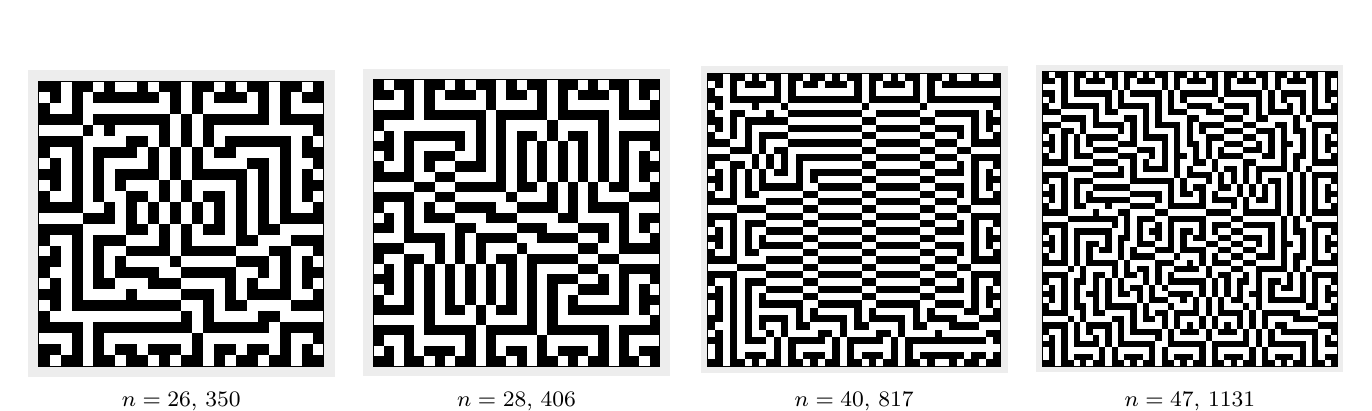
\begin{tikzpicture}
\begin{scope}[xshift=0.000cm]
\begin{scope}[x=0.1393cm,y=0.1393cm]
\fill[black!7] (-1,-1) rectangle (27,27);
\fill[white] (0,0) rectangle (26,26);
\draw[black,line width=.35pt] (0,0) rectangle (26,26);
\fill (0,25) rectangle (2,26);
\fill (3,25) rectangle (5,26);
\fill (6,25) rectangle (7,26);
\fill (9,25) rectangle (10,26);
\fill (11,25) rectangle (13,26);
\fill (14,25) rectangle (16,26);
\fill (17,25) rectangle (18,26);
\fill (19,25) rectangle (21,26);
\fill (22,25) rectangle (24,26);
\fill (25,25) rectangle (26,26);
\fill (1,24) rectangle (2,25);
\fill (3,24) rectangle (4,25);
\fill (5,24) rectangle (11,25);
\fill (12,24) rectangle (13,25);
\fill (14,24) rectangle (15,25);
\fill (16,24) rectangle (19,25);
\fill (20,24) rectangle (21,25);
\fill (22,24) rectangle (23,25);
\fill (24,24) rectangle (26,25);
\fill (0,23) rectangle (1,24);
\fill (3,23) rectangle (4,24);
\fill (12,23) rectangle (13,24);
\fill (14,23) rectangle (15,24);
\fill (20,23) rectangle (21,24);
\fill (22,23) rectangle (23,24);
\fill (0,22) rectangle (4,23);
\fill (5,22) rectangle (12,23);
\fill (13,22) rectangle (14,23);
\fill (15,22) rectangle (21,23);
\fill (22,22) rectangle (26,23);
\fill (4,21) rectangle (5,22);
\fill (6,21) rectangle (7,22);
\fill (11,21) rectangle (12,22);
\fill (13,21) rectangle (14,22);
\fill (15,21) rectangle (16,22);
\fill (25,21) rectangle (26,22);
\fill (0,20) rectangle (4,21);
\fill (8,20) rectangle (10,21);
\fill (11,20) rectangle (12,21);
\fill (13,20) rectangle (14,21);
\fill (15,20) rectangle (16,21);
\fill (17,20) rectangle (23,21);
\fill (24,20) rectangle (25,21);
\fill (0,19) rectangle (1,20);
\fill (3,19) rectangle (4,20);
\fill (5,19) rectangle (9,20);
\fill (10,19) rectangle (11,20);
\fill (12,19) rectangle (13,20);
\fill (14,19) rectangle (15,20);
\fill (16,19) rectangle (18,20);
\fill (22,19) rectangle (23,20);
\fill (24,19) rectangle (26,20);
\fill (1,18) rectangle (2,19);
\fill (3,18) rectangle (4,19);
\fill (5,18) rectangle (6,19);
\fill (10,18) rectangle (11,19);
\fill (12,18) rectangle (13,19);
\fill (14,18) rectangle (15,19);
\fill (19,18) rectangle (21,19);
\fill (22,18) rectangle (23,19);
\fill (25,18) rectangle (26,19);
\fill (0,17) rectangle (2,18);
\fill (3,17) rectangle (4,18);
\fill (5,17) rectangle (6,18);
\fill (7,17) rectangle (11,18);
\fill (12,17) rectangle (13,18);
\fill (14,17) rectangle (19,18);
\fill (20,17) rectangle (21,18);
\fill (22,17) rectangle (23,18);
\fill (24,17) rectangle (25,18);
\fill (1,16) rectangle (2,17);
\fill (3,16) rectangle (4,17);
\fill (5,16) rectangle (6,17);
\fill (7,16) rectangle (8,17);
\fill (11,16) rectangle (12,17);
\fill (13,16) rectangle (14,17);
\fill (18,16) rectangle (19,17);
\fill (20,16) rectangle (21,17);
\fill (22,16) rectangle (23,17);
\fill (24,16) rectangle (26,17);
\fill (0,15) rectangle (1,16);
\fill (3,15) rectangle (4,16);
\fill (5,15) rectangle (6,16);
\fill (8,15) rectangle (10,16);
\fill (11,15) rectangle (12,16);
\fill (13,15) rectangle (14,16);
\fill (15,15) rectangle (17,16);
\fill (18,15) rectangle (19,16);
\fill (20,15) rectangle (21,16);
\fill (22,15) rectangle (23,16);
\fill (24,15) rectangle (25,16);
\fill (0,14) rectangle (4,15);
\fill (6,14) rectangle (7,15);
\fill (8,14) rectangle (9,15);
\fill (10,14) rectangle (11,15);
\fill (12,14) rectangle (13,15);
\fill (14,14) rectangle (15,15);
\fill (16,14) rectangle (17,15);
\fill (18,14) rectangle (19,15);
\fill (20,14) rectangle (21,15);
\fill (22,14) rectangle (23,15);
\fill (25,14) rectangle (26,15);
\fill (4,13) rectangle (7,14);
\fill (8,13) rectangle (9,14);
\fill (10,13) rectangle (11,14);
\fill (12,13) rectangle (13,14);
\fill (14,13) rectangle (15,14);
\fill (16,13) rectangle (17,14);
\fill (18,13) rectangle (19,14);
\fill (20,13) rectangle (21,14);
\fill (22,13) rectangle (26,14);
\fill (0,12) rectangle (4,13);
\fill (8,12) rectangle (10,13);
\fill (11,12) rectangle (12,13);
\fill (13,12) rectangle (14,13);
\fill (15,12) rectangle (17,13);
\fill (18,12) rectangle (19,13);
\fill (20,12) rectangle (22,13);
\fill (0,11) rectangle (1,12);
\fill (3,11) rectangle (4,12);
\fill (5,11) rectangle (8,12);
\fill (11,11) rectangle (12,12);
\fill (13,11) rectangle (14,12);
\fill (18,11) rectangle (20,12);
\fill (23,11) rectangle (26,12);
\fill (1,10) rectangle (2,11);
\fill (3,10) rectangle (4,11);
\fill (5,10) rectangle (6,11);
\fill (8,10) rectangle (12,11);
\fill (13,10) rectangle (18,11);
\fill (21,10) rectangle (23,11);
\fill (25,10) rectangle (26,11);
\fill (0,9) rectangle (2,10);
\fill (3,9) rectangle (4,10);
\fill (5,9) rectangle (6,10);
\fill (7,9) rectangle (8,10);
\fill (12,9) rectangle (13,10);
\fill (18,9) rectangle (21,10);
\fill (22,9) rectangle (23,10);
\fill (24,9) rectangle (25,10);
\fill (0,8) rectangle (1,9);
\fill (3,8) rectangle (4,9);
\fill (5,8) rectangle (6,9);
\fill (7,8) rectangle (11,9);
\fill (13,8) rectangle (18,9);
\fill (20,8) rectangle (21,9);
\fill (22,8) rectangle (23,9);
\fill (24,8) rectangle (26,9);
\fill (1,7) rectangle (2,8);
\fill (3,7) rectangle (4,8);
\fill (5,7) rectangle (7,8);
\fill (10,7) rectangle (13,8);
\fill (17,7) rectangle (18,8);
\fill (19,7) rectangle (20,8);
\fill (22,7) rectangle (23,8);
\fill (24,7) rectangle (25,8);
\fill (0,6) rectangle (2,7);
\fill (3,6) rectangle (4,7);
\fill (8,6) rectangle (9,7);
\fill (13,6) rectangle (16,7);
\fill (17,6) rectangle (18,7);
\fill (19,6) rectangle (23,7);
\fill (25,6) rectangle (26,7);
\fill (1,5) rectangle (2,6);
\fill (3,5) rectangle (13,6);
\fill (15,5) rectangle (16,6);
\fill (17,5) rectangle (19,6);
\fill (23,5) rectangle (26,6);
\fill (0,4) rectangle (1,5);
\fill (13,4) rectangle (14,5);
\fill (15,4) rectangle (16,5);
\fill (20,4) rectangle (22,5);
\fill (0,3) rectangle (4,4);
\fill (5,3) rectangle (14,4);
\fill (15,3) rectangle (21,4);
\fill (22,3) rectangle (26,4);
\fill (3,2) rectangle (4,3);
\fill (5,2) rectangle (6,3);
\fill (14,2) rectangle (15,3);
\fill (22,2) rectangle (23,3);
\fill (25,2) rectangle (26,3);
\fill (0,1) rectangle (2,2);
\fill (3,1) rectangle (4,2);
\fill (5,1) rectangle (6,2);
\fill (7,1) rectangle (9,2);
\fill (10,1) rectangle (13,2);
\fill (14,1) rectangle (15,2);
\fill (16,1) rectangle (18,2);
\fill (19,1) rectangle (21,2);
\fill (22,1) rectangle (23,2);
\fill (24,1) rectangle (25,2);
\fill (0,0) rectangle (1,1);
\fill (2,0) rectangle (4,1);
\fill (5,0) rectangle (7,1);
\fill (8,0) rectangle (10,1);
\fill (11,0) rectangle (12,1);
\fill (13,0) rectangle (15,1);
\fill (16,0) rectangle (17,1);
\fill (18,0) rectangle (20,1);
\fill (21,0) rectangle (23,1);
\fill (24,0) rectangle (26,1);
\end{scope}
\node[align=center,font=\footnotesize] at (1.811,-0.45) {$n=26$, $350$};
\end{scope}
\begin{scope}[xshift=4.250cm]
\begin{scope}[x=0.1300cm,y=0.1300cm]
\fill[black!7] (-1,-1) rectangle (29,29);
\fill[white] (0,0) rectangle (28,28);
\draw[black,line width=.35pt] (0,0) rectangle (28,28);
\fill (0,27) rectangle (1,28);
\fill (2,27) rectangle (4,28);
\fill (5,27) rectangle (7,28);
\fill (8,27) rectangle (9,28);
\fill (10,27) rectangle (12,28);
\fill (13,27) rectangle (14,28);
\fill (15,27) rectangle (17,28);
\fill (18,27) rectangle (20,28);
\fill (21,27) rectangle (22,28);
\fill (23,27) rectangle (25,28);
\fill (26,27) rectangle (28,28);
\fill (0,26) rectangle (2,27);
\fill (3,26) rectangle (4,27);
\fill (5,26) rectangle (6,27);
\fill (7,26) rectangle (10,27);
\fill (11,26) rectangle (12,27);
\fill (13,26) rectangle (15,27);
\fill (16,26) rectangle (17,27);
\fill (18,26) rectangle (19,27);
\fill (20,26) rectangle (23,27);
\fill (24,26) rectangle (25,27);
\fill (26,26) rectangle (27,27);
\fill (3,25) rectangle (4,26);
\fill (5,25) rectangle (6,26);
\fill (11,25) rectangle (12,26);
\fill (16,25) rectangle (17,26);
\fill (18,25) rectangle (19,26);
\fill (24,25) rectangle (25,26);
\fill (27,25) rectangle (28,26);
\fill (0,24) rectangle (4,25);
\fill (5,24) rectangle (11,25);
\fill (12,24) rectangle (17,25);
\fill (18,24) rectangle (23,25);
\fill (24,24) rectangle (28,25);
\fill (0,23) rectangle (1,24);
\fill (10,23) rectangle (11,24);
\fill (12,23) rectangle (13,24);
\fill (17,23) rectangle (18,24);
\fill (22,23) rectangle (23,24);
\fill (1,22) rectangle (2,23);
\fill (3,22) rectangle (9,23);
\fill (10,22) rectangle (11,23);
\fill (12,22) rectangle (13,23);
\fill (14,22) rectangle (16,23);
\fill (17,22) rectangle (18,23);
\fill (19,22) rectangle (21,23);
\fill (22,22) rectangle (23,23);
\fill (24,22) rectangle (28,23);
\fill (0,21) rectangle (2,22);
\fill (3,21) rectangle (4,22);
\fill (8,21) rectangle (9,22);
\fill (10,21) rectangle (11,22);
\fill (12,21) rectangle (13,22);
\fill (14,21) rectangle (15,22);
\fill (16,21) rectangle (17,22);
\fill (18,21) rectangle (19,22);
\fill (20,21) rectangle (21,22);
\fill (22,21) rectangle (23,22);
\fill (24,21) rectangle (25,22);
\fill (27,21) rectangle (28,22);
\fill (1,20) rectangle (2,21);
\fill (3,20) rectangle (4,21);
\fill (5,20) rectangle (8,21);
\fill (10,20) rectangle (11,21);
\fill (12,20) rectangle (13,21);
\fill (14,20) rectangle (15,21);
\fill (16,20) rectangle (17,21);
\fill (18,20) rectangle (19,21);
\fill (20,20) rectangle (21,21);
\fill (22,20) rectangle (23,21);
\fill (24,20) rectangle (25,21);
\fill (26,20) rectangle (27,21);
\fill (0,19) rectangle (1,20);
\fill (3,19) rectangle (4,20);
\fill (5,19) rectangle (6,20);
\fill (8,19) rectangle (11,20);
\fill (12,19) rectangle (13,20);
\fill (14,19) rectangle (15,20);
\fill (16,19) rectangle (17,20);
\fill (18,19) rectangle (19,20);
\fill (20,19) rectangle (21,20);
\fill (22,19) rectangle (23,20);
\fill (24,19) rectangle (25,20);
\fill (26,19) rectangle (28,20);
\fill (0,18) rectangle (4,19);
\fill (6,18) rectangle (8,19);
\fill (12,18) rectangle (13,19);
\fill (14,18) rectangle (15,19);
\fill (16,18) rectangle (17,19);
\fill (18,18) rectangle (19,19);
\fill (20,18) rectangle (21,19);
\fill (22,18) rectangle (23,19);
\fill (24,18) rectangle (25,19);
\fill (26,18) rectangle (27,19);
\fill (4,17) rectangle (6,18);
\fill (8,17) rectangle (13,18);
\fill (14,17) rectangle (16,18);
\fill (17,17) rectangle (18,18);
\fill (19,17) rectangle (20,18);
\fill (21,17) rectangle (22,18);
\fill (23,17) rectangle (25,18);
\fill (27,17) rectangle (28,18);
\fill (0,16) rectangle (4,17);
\fill (6,16) rectangle (8,17);
\fill (13,16) rectangle (14,17);
\fill (17,16) rectangle (18,17);
\fill (19,16) rectangle (20,17);
\fill (21,16) rectangle (22,17);
\fill (25,16) rectangle (28,17);
\fill (0,15) rectangle (1,16);
\fill (3,15) rectangle (4,16);
\fill (5,15) rectangle (6,16);
\fill (8,15) rectangle (12,16);
\fill (14,15) rectangle (18,16);
\fill (19,15) rectangle (20,16);
\fill (21,15) rectangle (25,16);
\fill (1,14) rectangle (2,15);
\fill (3,14) rectangle (4,15);
\fill (5,14) rectangle (8,15);
\fill (11,14) rectangle (14,15);
\fill (18,14) rectangle (20,15);
\fill (24,14) rectangle (25,15);
\fill (26,14) rectangle (28,15);
\fill (0,13) rectangle (2,14);
\fill (3,13) rectangle (4,14);
\fill (8,13) rectangle (10,14);
\fill (14,13) rectangle (17,14);
\fill (20,13) rectangle (23,14);
\fill (24,13) rectangle (25,14);
\fill (26,13) rectangle (27,14);
\fill (3,12) rectangle (7,13);
\fill (8,12) rectangle (9,13);
\fill (10,12) rectangle (14,13);
\fill (16,12) rectangle (20,13);
\fill (22,12) rectangle (23,13);
\fill (24,12) rectangle (25,13);
\fill (27,12) rectangle (28,13);
\fill (0,11) rectangle (3,12);
\fill (6,11) rectangle (7,12);
\fill (8,11) rectangle (9,12);
\fill (10,11) rectangle (11,12);
\fill (14,11) rectangle (15,12);
\fill (20,11) rectangle (22,12);
\fill (24,11) rectangle (28,12);
\fill (0,10) rectangle (1,11);
\fill (3,10) rectangle (5,11);
\fill (6,10) rectangle (7,11);
\fill (8,10) rectangle (9,11);
\fill (10,10) rectangle (11,11);
\fill (12,10) rectangle (14,11);
\fill (15,10) rectangle (20,11);
\fill (22,10) rectangle (24,11);
\fill (1,9) rectangle (2,10);
\fill (3,9) rectangle (4,10);
\fill (5,9) rectangle (6,10);
\fill (7,9) rectangle (8,10);
\fill (9,9) rectangle (10,10);
\fill (11,9) rectangle (12,10);
\fill (13,9) rectangle (14,10);
\fill (15,9) rectangle (16,10);
\fill (20,9) rectangle (22,10);
\fill (24,9) rectangle (28,10);
\fill (0,8) rectangle (2,9);
\fill (3,8) rectangle (4,9);
\fill (5,8) rectangle (6,9);
\fill (7,8) rectangle (8,9);
\fill (9,8) rectangle (10,9);
\fill (11,8) rectangle (12,9);
\fill (13,8) rectangle (14,9);
\fill (15,8) rectangle (16,9);
\fill (17,8) rectangle (20,9);
\fill (22,8) rectangle (23,9);
\fill (24,8) rectangle (25,9);
\fill (27,8) rectangle (28,9);
\fill (1,7) rectangle (2,8);
\fill (3,7) rectangle (4,8);
\fill (5,7) rectangle (6,8);
\fill (7,7) rectangle (8,8);
\fill (9,7) rectangle (10,8);
\fill (11,7) rectangle (12,8);
\fill (13,7) rectangle (14,8);
\fill (15,7) rectangle (16,8);
\fill (17,7) rectangle (18,8);
\fill (20,7) rectangle (23,8);
\fill (24,7) rectangle (25,8);
\fill (26,7) rectangle (27,8);
\fill (0,6) rectangle (1,7);
\fill (3,6) rectangle (4,7);
\fill (5,6) rectangle (6,7);
\fill (7,6) rectangle (8,7);
\fill (9,6) rectangle (10,7);
\fill (11,6) rectangle (12,7);
\fill (13,6) rectangle (14,7);
\fill (15,6) rectangle (16,7);
\fill (17,6) rectangle (18,7);
\fill (19,6) rectangle (20,7);
\fill (24,6) rectangle (25,7);
\fill (26,6) rectangle (28,7);
\fill (0,5) rectangle (4,6);
\fill (5,5) rectangle (6,6);
\fill (7,5) rectangle (9,6);
\fill (10,5) rectangle (11,6);
\fill (12,5) rectangle (14,6);
\fill (15,5) rectangle (16,6);
\fill (17,5) rectangle (18,6);
\fill (19,5) rectangle (25,6);
\fill (26,5) rectangle (27,6);
\fill (5,4) rectangle (6,5);
\fill (10,4) rectangle (11,5);
\fill (15,4) rectangle (16,5);
\fill (17,4) rectangle (18,5);
\fill (27,4) rectangle (28,5);
\fill (0,3) rectangle (4,4);
\fill (5,3) rectangle (10,4);
\fill (11,3) rectangle (16,4);
\fill (17,3) rectangle (23,4);
\fill (24,3) rectangle (28,4);
\fill (0,2) rectangle (1,3);
\fill (3,2) rectangle (4,3);
\fill (9,2) rectangle (10,3);
\fill (11,2) rectangle (12,3);
\fill (16,2) rectangle (17,3);
\fill (22,2) rectangle (23,3);
\fill (24,2) rectangle (25,3);
\fill (1,1) rectangle (2,2);
\fill (3,1) rectangle (4,2);
\fill (5,1) rectangle (8,2);
\fill (9,1) rectangle (10,2);
\fill (11,1) rectangle (12,2);
\fill (13,1) rectangle (15,2);
\fill (16,1) rectangle (17,2);
\fill (18,1) rectangle (21,2);
\fill (22,1) rectangle (23,2);
\fill (24,1) rectangle (25,2);
\fill (26,1) rectangle (28,2);
\fill (0,0) rectangle (2,1);
\fill (3,0) rectangle (5,1);
\fill (6,0) rectangle (7,1);
\fill (8,0) rectangle (10,1);
\fill (11,0) rectangle (13,1);
\fill (14,0) rectangle (15,1);
\fill (16,0) rectangle (18,1);
\fill (19,0) rectangle (20,1);
\fill (21,0) rectangle (23,1);
\fill (24,0) rectangle (26,1);
\fill (27,0) rectangle (28,1);
\end{scope}
\node[align=center,font=\footnotesize] at (1.820,-0.45) {$n=28$, $406$};
\end{scope}
\begin{scope}[xshift=8.500cm]
\begin{scope}[x=0.0929cm,y=0.0929cm]
\fill[black!7] (-1,-1) rectangle (41,41);
\fill[white] (0,0) rectangle (40,40);
\draw[black,line width=.35pt] (0,0) rectangle (40,40);
\fill (0,39) rectangle (2,40);
\fill (3,39) rectangle (5,40);
\fill (6,39) rectangle (7,40);
\fill (8,39) rectangle (10,40);
\fill (11,39) rectangle (13,40);
\fill (14,39) rectangle (16,40);
\fill (17,39) rectangle (18,40);
\fill (19,39) rectangle (21,40);
\fill (22,39) rectangle (24,40);
\fill (25,39) rectangle (26,40);
\fill (27,39) rectangle (29,40);
\fill (30,39) rectangle (32,40);
\fill (33,39) rectangle (34,40);
\fill (36,39) rectangle (37,40);
\fill (39,39) rectangle (40,40);
\fill (1,38) rectangle (2,39);
\fill (3,38) rectangle (4,39);
\fill (5,38) rectangle (8,39);
\fill (9,38) rectangle (10,39);
\fill (11,38) rectangle (12,39);
\fill (13,38) rectangle (15,39);
\fill (16,38) rectangle (19,39);
\fill (20,38) rectangle (21,39);
\fill (22,38) rectangle (23,39);
\fill (24,38) rectangle (27,39);
\fill (28,38) rectangle (29,39);
\fill (30,38) rectangle (31,39);
\fill (32,38) rectangle (40,39);
\fill (0,37) rectangle (1,38);
\fill (3,37) rectangle (4,38);
\fill (9,37) rectangle (10,38);
\fill (11,37) rectangle (12,38);
\fill (20,37) rectangle (21,38);
\fill (22,37) rectangle (23,38);
\fill (28,37) rectangle (29,38);
\fill (30,37) rectangle (31,38);
\fill (0,36) rectangle (2,37);
\fill (3,36) rectangle (10,37);
\fill (11,36) rectangle (21,37);
\fill (22,36) rectangle (29,37);
\fill (30,36) rectangle (40,37);
\fill (1,35) rectangle (2,36);
\fill (6,35) rectangle (7,36);
\fill (10,35) rectangle (11,36);
\fill (21,35) rectangle (22,36);
\fill (29,35) rectangle (30,36);
\fill (39,35) rectangle (40,36);
\fill (0,34) rectangle (1,35);
\fill (3,34) rectangle (5,35);
\fill (8,34) rectangle (9,35);
\fill (11,34) rectangle (21,35);
\fill (23,34) rectangle (29,35);
\fill (31,34) rectangle (37,35);
\fill (38,34) rectangle (39,35);
\fill (0,33) rectangle (2,34);
\fill (3,33) rectangle (4,34);
\fill (5,33) rectangle (11,34);
\fill (21,33) rectangle (23,34);
\fill (29,33) rectangle (31,34);
\fill (36,33) rectangle (37,34);
\fill (38,33) rectangle (40,34);
\fill (1,32) rectangle (2,33);
\fill (3,32) rectangle (4,33);
\fill (5,32) rectangle (6,33);
\fill (11,32) rectangle (21,33);
\fill (23,32) rectangle (29,33);
\fill (31,32) rectangle (35,33);
\fill (36,32) rectangle (37,33);
\fill (38,32) rectangle (39,33);
\fill (0,31) rectangle (1,32);
\fill (3,31) rectangle (4,32);
\fill (5,31) rectangle (6,32);
\fill (7,31) rectangle (11,32);
\fill (21,31) rectangle (23,32);
\fill (29,31) rectangle (31,32);
\fill (34,31) rectangle (35,32);
\fill (36,31) rectangle (37,32);
\fill (39,31) rectangle (40,32);
\fill (0,30) rectangle (3,31);
\fill (5,30) rectangle (6,31);
\fill (7,30) rectangle (8,31);
\fill (11,30) rectangle (21,31);
\fill (23,30) rectangle (29,31);
\fill (31,30) rectangle (34,31);
\fill (36,30) rectangle (40,31);
\fill (3,29) rectangle (6,30);
\fill (7,29) rectangle (8,30);
\fill (9,29) rectangle (11,30);
\fill (21,29) rectangle (23,30);
\fill (29,29) rectangle (31,30);
\fill (34,29) rectangle (36,30);
\fill (0,28) rectangle (3,29);
\fill (6,28) rectangle (7,29);
\fill (8,28) rectangle (9,29);
\fill (10,28) rectangle (11,29);
\fill (12,28) rectangle (21,29);
\fill (23,28) rectangle (29,29);
\fill (31,28) rectangle (34,29);
\fill (36,28) rectangle (40,29);
\fill (0,27) rectangle (1,28);
\fill (3,27) rectangle (5,28);
\fill (6,27) rectangle (7,28);
\fill (8,27) rectangle (9,28);
\fill (10,27) rectangle (11,28);
\fill (12,27) rectangle (13,28);
\fill (21,27) rectangle (23,28);
\fill (29,27) rectangle (31,28);
\fill (34,27) rectangle (35,28);
\fill (36,27) rectangle (37,28);
\fill (39,27) rectangle (40,28);
\fill (1,26) rectangle (2,27);
\fill (3,26) rectangle (4,27);
\fill (5,26) rectangle (6,27);
\fill (7,26) rectangle (8,27);
\fill (9,26) rectangle (11,27);
\fill (12,26) rectangle (13,27);
\fill (14,26) rectangle (21,27);
\fill (23,26) rectangle (29,27);
\fill (31,26) rectangle (35,27);
\fill (36,26) rectangle (37,27);
\fill (38,26) rectangle (39,27);
\fill (0,25) rectangle (2,26);
\fill (3,25) rectangle (4,26);
\fill (5,25) rectangle (6,26);
\fill (7,25) rectangle (8,26);
\fill (12,25) rectangle (13,26);
\fill (14,25) rectangle (15,26);
\fill (21,25) rectangle (23,26);
\fill (29,25) rectangle (31,26);
\fill (36,25) rectangle (37,26);
\fill (38,25) rectangle (40,26);
\fill (1,24) rectangle (2,25);
\fill (3,24) rectangle (4,25);
\fill (5,24) rectangle (6,25);
\fill (7,24) rectangle (13,25);
\fill (15,24) rectangle (21,25);
\fill (23,24) rectangle (29,25);
\fill (31,24) rectangle (35,25);
\fill (36,24) rectangle (37,25);
\fill (38,24) rectangle (39,25);
\fill (0,23) rectangle (1,24);
\fill (3,23) rectangle (4,24);
\fill (5,23) rectangle (7,24);
\fill (13,23) rectangle (15,24);
\fill (21,23) rectangle (23,24);
\fill (29,23) rectangle (31,24);
\fill (34,23) rectangle (35,24);
\fill (36,23) rectangle (37,24);
\fill (39,23) rectangle (40,24);
\fill (0,22) rectangle (4,23);
\fill (8,22) rectangle (13,23);
\fill (15,22) rectangle (21,23);
\fill (23,22) rectangle (29,23);
\fill (31,22) rectangle (34,23);
\fill (36,22) rectangle (40,23);
\fill (4,21) rectangle (8,22);
\fill (13,21) rectangle (15,22);
\fill (21,21) rectangle (23,22);
\fill (29,21) rectangle (31,22);
\fill (34,21) rectangle (36,22);
\fill (0,20) rectangle (4,21);
\fill (8,20) rectangle (13,21);
\fill (15,20) rectangle (21,21);
\fill (23,20) rectangle (29,21);
\fill (31,20) rectangle (34,21);
\fill (36,20) rectangle (40,21);
\fill (0,19) rectangle (1,20);
\fill (3,19) rectangle (4,20);
\fill (5,19) rectangle (8,20);
\fill (13,19) rectangle (15,20);
\fill (21,19) rectangle (23,20);
\fill (29,19) rectangle (31,20);
\fill (34,19) rectangle (35,20);
\fill (36,19) rectangle (37,20);
\fill (39,19) rectangle (40,20);
\fill (1,18) rectangle (2,19);
\fill (3,18) rectangle (4,19);
\fill (5,18) rectangle (6,19);
\fill (8,18) rectangle (13,19);
\fill (15,18) rectangle (21,19);
\fill (23,18) rectangle (29,19);
\fill (31,18) rectangle (35,19);
\fill (36,18) rectangle (37,19);
\fill (38,18) rectangle (39,19);
\fill (0,17) rectangle (2,18);
\fill (3,17) rectangle (4,18);
\fill (5,17) rectangle (6,18);
\fill (7,17) rectangle (8,18);
\fill (13,17) rectangle (15,18);
\fill (21,17) rectangle (23,18);
\fill (29,17) rectangle (31,18);
\fill (36,17) rectangle (37,18);
\fill (38,17) rectangle (40,18);
\fill (1,16) rectangle (2,17);
\fill (3,16) rectangle (4,17);
\fill (5,16) rectangle (6,17);
\fill (7,16) rectangle (13,17);
\fill (15,16) rectangle (21,17);
\fill (23,16) rectangle (29,17);
\fill (31,16) rectangle (35,17);
\fill (36,16) rectangle (37,17);
\fill (38,16) rectangle (39,17);
\fill (0,15) rectangle (1,16);
\fill (3,15) rectangle (4,16);
\fill (5,15) rectangle (7,16);
\fill (13,15) rectangle (15,16);
\fill (21,15) rectangle (23,16);
\fill (29,15) rectangle (31,16);
\fill (34,15) rectangle (35,16);
\fill (36,15) rectangle (37,16);
\fill (39,15) rectangle (40,16);
\fill (0,14) rectangle (4,15);
\fill (8,14) rectangle (13,15);
\fill (15,14) rectangle (21,15);
\fill (23,14) rectangle (29,15);
\fill (31,14) rectangle (34,15);
\fill (36,14) rectangle (40,15);
\fill (4,13) rectangle (8,14);
\fill (13,13) rectangle (15,14);
\fill (21,13) rectangle (23,14);
\fill (29,13) rectangle (31,14);
\fill (34,13) rectangle (36,14);
\fill (0,12) rectangle (4,13);
\fill (8,12) rectangle (13,13);
\fill (15,12) rectangle (21,13);
\fill (23,12) rectangle (29,13);
\fill (31,12) rectangle (34,13);
\fill (36,12) rectangle (40,13);
\fill (0,11) rectangle (1,12);
\fill (3,11) rectangle (4,12);
\fill (5,11) rectangle (8,12);
\fill (13,11) rectangle (15,12);
\fill (21,11) rectangle (23,12);
\fill (29,11) rectangle (31,12);
\fill (34,11) rectangle (35,12);
\fill (36,11) rectangle (37,12);
\fill (39,11) rectangle (40,12);
\fill (1,10) rectangle (2,11);
\fill (3,10) rectangle (4,11);
\fill (5,10) rectangle (6,11);
\fill (8,10) rectangle (13,11);
\fill (15,10) rectangle (21,11);
\fill (23,10) rectangle (29,11);
\fill (31,10) rectangle (35,11);
\fill (36,10) rectangle (37,11);
\fill (38,10) rectangle (39,11);
\fill (0,9) rectangle (2,10);
\fill (3,9) rectangle (4,10);
\fill (5,9) rectangle (6,10);
\fill (7,9) rectangle (8,10);
\fill (13,9) rectangle (15,10);
\fill (21,9) rectangle (23,10);
\fill (29,9) rectangle (31,10);
\fill (36,9) rectangle (37,10);
\fill (38,9) rectangle (40,10);
\fill (1,8) rectangle (2,9);
\fill (3,8) rectangle (4,9);
\fill (5,8) rectangle (6,9);
\fill (7,8) rectangle (13,9);
\fill (15,8) rectangle (21,9);
\fill (23,8) rectangle (29,9);
\fill (31,8) rectangle (35,9);
\fill (36,8) rectangle (37,9);
\fill (38,8) rectangle (39,9);
\fill (1,7) rectangle (2,8);
\fill (3,7) rectangle (4,8);
\fill (5,7) rectangle (6,8);
\fill (12,7) rectangle (13,8);
\fill (14,7) rectangle (15,8);
\fill (20,7) rectangle (21,8);
\fill (22,7) rectangle (23,8);
\fill (28,7) rectangle (29,8);
\fill (30,7) rectangle (31,8);
\fill (35,7) rectangle (37,8);
\fill (39,7) rectangle (40,8);
\fill (0,6) rectangle (2,7);
\fill (3,6) rectangle (4,7);
\fill (5,6) rectangle (6,7);
\fill (7,6) rectangle (11,7);
\fill (12,6) rectangle (13,7);
\fill (14,6) rectangle (19,7);
\fill (20,6) rectangle (21,7);
\fill (22,6) rectangle (27,7);
\fill (28,6) rectangle (29,7);
\fill (30,6) rectangle (34,7);
\fill (37,6) rectangle (40,7);
\fill (0,5) rectangle (1,6);
\fill (3,5) rectangle (4,6);
\fill (5,5) rectangle (6,6);
\fill (7,5) rectangle (8,6);
\fill (10,5) rectangle (11,6);
\fill (12,5) rectangle (14,6);
\fill (18,5) rectangle (19,6);
\fill (20,5) rectangle (22,6);
\fill (26,5) rectangle (27,6);
\fill (28,5) rectangle (30,6);
\fill (33,5) rectangle (37,6);
\fill (1,4) rectangle (2,5);
\fill (3,4) rectangle (4,5);
\fill (5,4) rectangle (6,5);
\fill (8,4) rectangle (9,5);
\fill (10,4) rectangle (11,5);
\fill (15,4) rectangle (17,5);
\fill (18,4) rectangle (19,5);
\fill (23,4) rectangle (25,5);
\fill (26,4) rectangle (27,5);
\fill (31,4) rectangle (32,5);
\fill (38,4) rectangle (40,5);
\fill (0,3) rectangle (2,4);
\fill (3,3) rectangle (4,4);
\fill (5,3) rectangle (8,4);
\fill (9,3) rectangle (10,4);
\fill (11,3) rectangle (16,4);
\fill (17,3) rectangle (18,4);
\fill (19,3) rectangle (24,4);
\fill (25,3) rectangle (26,4);
\fill (27,3) rectangle (38,4);
\fill (39,3) rectangle (40,4);
\fill (1,2) rectangle (2,3);
\fill (3,2) rectangle (4,3);
\fill (9,2) rectangle (10,3);
\fill (11,2) rectangle (12,3);
\fill (17,2) rectangle (18,3);
\fill (19,2) rectangle (20,3);
\fill (25,2) rectangle (26,3);
\fill (27,2) rectangle (28,3);
\fill (1,1) rectangle (2,2);
\fill (3,1) rectangle (4,2);
\fill (5,1) rectangle (8,2);
\fill (9,1) rectangle (10,2);
\fill (11,1) rectangle (12,2);
\fill (13,1) rectangle (16,2);
\fill (17,1) rectangle (18,2);
\fill (19,1) rectangle (20,2);
\fill (21,1) rectangle (24,2);
\fill (25,1) rectangle (26,2);
\fill (27,1) rectangle (28,2);
\fill (29,1) rectangle (35,2);
\fill (36,1) rectangle (38,2);
\fill (39,1) rectangle (40,2);
\fill (0,0) rectangle (2,1);
\fill (3,0) rectangle (5,1);
\fill (6,0) rectangle (7,1);
\fill (8,0) rectangle (10,1);
\fill (11,0) rectangle (13,1);
\fill (14,0) rectangle (15,1);
\fill (16,0) rectangle (18,1);
\fill (19,0) rectangle (21,1);
\fill (22,0) rectangle (23,1);
\fill (24,0) rectangle (26,1);
\fill (27,0) rectangle (29,1);
\fill (30,0) rectangle (31,1);
\fill (33,0) rectangle (34,1);
\fill (35,0) rectangle (37,1);
\fill (38,0) rectangle (40,1);
\end{scope}
\node[align=center,font=\footnotesize] at (1.857,-0.45) {$n=40$, $817$};
\end{scope}
\begin{scope}[xshift=12.750cm]
\begin{scope}[x=0.0796cm,y=0.0796cm]
\fill[black!7] (-1,-1) rectangle (48,48);
\fill[white] (0,0) rectangle (47,47);
\draw[black,line width=.35pt] (0,0) rectangle (47,47);
\fill (0,46) rectangle (1,47);
\fill (2,46) rectangle (4,47);
\fill (5,46) rectangle (7,47);
\fill (8,46) rectangle (9,47);
\fill (10,46) rectangle (12,47);
\fill (13,46) rectangle (15,47);
\fill (16,46) rectangle (17,47);
\fill (18,46) rectangle (20,47);
\fill (21,46) rectangle (23,47);
\fill (24,46) rectangle (25,47);
\fill (26,46) rectangle (28,47);
\fill (29,46) rectangle (31,47);
\fill (32,46) rectangle (33,47);
\fill (34,46) rectangle (36,47);
\fill (37,46) rectangle (39,47);
\fill (40,46) rectangle (41,47);
\fill (42,46) rectangle (44,47);
\fill (45,46) rectangle (47,47);
\fill (0,45) rectangle (2,46);
\fill (3,45) rectangle (4,46);
\fill (5,45) rectangle (6,46);
\fill (7,45) rectangle (10,46);
\fill (11,45) rectangle (12,46);
\fill (13,45) rectangle (14,46);
\fill (15,45) rectangle (18,46);
\fill (19,45) rectangle (20,46);
\fill (21,45) rectangle (22,46);
\fill (23,45) rectangle (26,46);
\fill (27,45) rectangle (28,46);
\fill (29,45) rectangle (30,46);
\fill (31,45) rectangle (34,46);
\fill (35,45) rectangle (36,46);
\fill (37,45) rectangle (38,46);
\fill (39,45) rectangle (42,46);
\fill (43,45) rectangle (44,46);
\fill (45,45) rectangle (46,46);
\fill (3,44) rectangle (4,45);
\fill (5,44) rectangle (6,45);
\fill (11,44) rectangle (12,45);
\fill (13,44) rectangle (14,45);
\fill (19,44) rectangle (20,45);
\fill (21,44) rectangle (22,45);
\fill (27,44) rectangle (28,45);
\fill (29,44) rectangle (30,45);
\fill (35,44) rectangle (36,45);
\fill (37,44) rectangle (38,45);
\fill (43,44) rectangle (44,45);
\fill (45,44) rectangle (46,45);
\fill (0,43) rectangle (2,44);
\fill (3,43) rectangle (4,44);
\fill (5,43) rectangle (11,44);
\fill (12,43) rectangle (13,44);
\fill (14,43) rectangle (19,44);
\fill (20,43) rectangle (21,44);
\fill (22,43) rectangle (28,44);
\fill (29,43) rectangle (35,44);
\fill (36,43) rectangle (37,44);
\fill (38,43) rectangle (42,44);
\fill (43,43) rectangle (44,44);
\fill (45,43) rectangle (47,44);
\fill (1,42) rectangle (2,43);
\fill (3,42) rectangle (4,43);
\fill (10,42) rectangle (11,43);
\fill (12,42) rectangle (13,43);
\fill (18,42) rectangle (19,43);
\fill (20,42) rectangle (21,43);
\fill (22,42) rectangle (23,43);
\fill (28,42) rectangle (29,43);
\fill (34,42) rectangle (35,43);
\fill (36,42) rectangle (37,43);
\fill (38,42) rectangle (39,43);
\fill (41,42) rectangle (42,43);
\fill (43,42) rectangle (44,43);
\fill (45,42) rectangle (46,43);
\fill (0,41) rectangle (1,42);
\fill (3,41) rectangle (9,42);
\fill (10,41) rectangle (11,42);
\fill (12,41) rectangle (17,42);
\fill (18,41) rectangle (19,42);
\fill (20,41) rectangle (21,42);
\fill (23,41) rectangle (27,42);
\fill (29,41) rectangle (33,42);
\fill (34,41) rectangle (35,42);
\fill (36,41) rectangle (37,42);
\fill (39,41) rectangle (40,42);
\fill (41,41) rectangle (42,42);
\fill (43,41) rectangle (44,42);
\fill (46,41) rectangle (47,42);
\fill (0,40) rectangle (3,41);
\fill (8,40) rectangle (9,41);
\fill (10,40) rectangle (12,41);
\fill (16,40) rectangle (17,41);
\fill (18,40) rectangle (19,41);
\fill (20,40) rectangle (23,41);
\fill (26,40) rectangle (29,41);
\fill (32,40) rectangle (33,41);
\fill (34,40) rectangle (35,41);
\fill (36,40) rectangle (40,41);
\fill (41,40) rectangle (42,41);
\fill (43,40) rectangle (47,41);
\fill (3,39) rectangle (7,40);
\fill (8,39) rectangle (9,40);
\fill (13,39) rectangle (15,40);
\fill (16,39) rectangle (17,40);
\fill (18,39) rectangle (19,40);
\fill (23,39) rectangle (25,40);
\fill (29,39) rectangle (32,40);
\fill (34,39) rectangle (36,40);
\fill (40,39) rectangle (41,40);
\fill (42,39) rectangle (43,40);
\fill (0,38) rectangle (3,39);
\fill (6,38) rectangle (7,39);
\fill (8,38) rectangle (13,39);
\fill (14,38) rectangle (15,39);
\fill (16,38) rectangle (17,39);
\fill (18,38) rectangle (22,39);
\fill (23,38) rectangle (24,39);
\fill (25,38) rectangle (29,39);
\fill (32,38) rectangle (34,39);
\fill (37,38) rectangle (39,39);
\fill (40,38) rectangle (41,39);
\fill (43,38) rectangle (47,39);
\fill (0,37) rectangle (1,38);
\fill (3,37) rectangle (5,38);
\fill (6,37) rectangle (7,38);
\fill (12,37) rectangle (13,38);
\fill (14,37) rectangle (15,38);
\fill (16,37) rectangle (17,38);
\fill (21,37) rectangle (22,38);
\fill (23,37) rectangle (24,38);
\fill (25,37) rectangle (26,38);
\fill (29,37) rectangle (32,38);
\fill (34,37) rectangle (37,38);
\fill (38,37) rectangle (39,38);
\fill (40,37) rectangle (42,38);
\fill (43,37) rectangle (44,38);
\fill (46,37) rectangle (47,38);
\fill (1,36) rectangle (2,37);
\fill (3,36) rectangle (4,37);
\fill (5,36) rectangle (6,37);
\fill (7,36) rectangle (12,37);
\fill (14,36) rectangle (15,37);
\fill (16,36) rectangle (20,37);
\fill (21,36) rectangle (22,37);
\fill (23,36) rectangle (24,37);
\fill (26,36) rectangle (29,37);
\fill (32,36) rectangle (34,37);
\fill (36,36) rectangle (37,37);
\fill (38,36) rectangle (39,37);
\fill (41,36) rectangle (42,37);
\fill (43,36) rectangle (44,37);
\fill (45,36) rectangle (46,37);
\fill (0,35) rectangle (2,36);
\fill (3,35) rectangle (4,36);
\fill (5,35) rectangle (6,36);
\fill (7,35) rectangle (8,36);
\fill (12,35) rectangle (15,36);
\fill (19,35) rectangle (20,36);
\fill (21,35) rectangle (22,36);
\fill (23,35) rectangle (25,36);
\fill (26,35) rectangle (27,36);
\fill (29,35) rectangle (32,36);
\fill (34,35) rectangle (35,36);
\fill (36,35) rectangle (37,36);
\fill (38,35) rectangle (40,36);
\fill (41,35) rectangle (42,36);
\fill (43,35) rectangle (44,36);
\fill (45,35) rectangle (47,36);
\fill (1,34) rectangle (2,35);
\fill (3,34) rectangle (4,35);
\fill (5,34) rectangle (6,35);
\fill (8,34) rectangle (12,35);
\fill (15,34) rectangle (18,35);
\fill (19,34) rectangle (20,35);
\fill (21,34) rectangle (22,35);
\fill (24,34) rectangle (25,35);
\fill (26,34) rectangle (27,35);
\fill (28,34) rectangle (29,35);
\fill (32,34) rectangle (35,35);
\fill (36,34) rectangle (37,35);
\fill (38,34) rectangle (39,35);
\fill (41,34) rectangle (42,35);
\fill (43,34) rectangle (44,35);
\fill (45,34) rectangle (46,35);
\fill (0,33) rectangle (1,34);
\fill (3,33) rectangle (4,34);
\fill (5,33) rectangle (8,34);
\fill (12,33) rectangle (15,34);
\fill (17,33) rectangle (18,34);
\fill (19,33) rectangle (20,34);
\fill (21,33) rectangle (23,34);
\fill (24,33) rectangle (25,34);
\fill (26,33) rectangle (27,34);
\fill (28,33) rectangle (32,34);
\fill (35,33) rectangle (37,34);
\fill (38,33) rectangle (39,34);
\fill (40,33) rectangle (42,34);
\fill (43,33) rectangle (44,34);
\fill (46,33) rectangle (47,34);
\fill (0,32) rectangle (4,33);
\fill (8,32) rectangle (12,33);
\fill (14,32) rectangle (15,33);
\fill (16,32) rectangle (17,33);
\fill (19,32) rectangle (20,33);
\fill (21,32) rectangle (22,33);
\fill (24,32) rectangle (26,33);
\fill (27,32) rectangle (28,33);
\fill (32,32) rectangle (34,33);
\fill (38,32) rectangle (39,33);
\fill (40,32) rectangle (41,33);
\fill (43,32) rectangle (47,33);
\fill (4,31) rectangle (8,32);
\fill (12,31) rectangle (13,32);
\fill (14,31) rectangle (15,32);
\fill (16,31) rectangle (20,32);
\fill (21,31) rectangle (22,32);
\fill (23,31) rectangle (24,32);
\fill (27,31) rectangle (28,32);
\fill (29,31) rectangle (31,32);
\fill (32,31) rectangle (33,32);
\fill (34,31) rectangle (39,32);
\fill (40,31) rectangle (41,32);
\fill (42,31) rectangle (43,32);
\fill (0,30) rectangle (4,31);
\fill (8,30) rectangle (13,31);
\fill (14,30) rectangle (15,31);
\fill (21,30) rectangle (22,31);
\fill (23,30) rectangle (27,31);
\fill (28,30) rectangle (29,31);
\fill (30,30) rectangle (31,31);
\fill (32,30) rectangle (33,31);
\fill (34,30) rectangle (35,31);
\fill (39,30) rectangle (40,31);
\fill (41,30) rectangle (42,31);
\fill (43,30) rectangle (47,31);
\fill (0,29) rectangle (1,30);
\fill (3,29) rectangle (4,30);
\fill (5,29) rectangle (8,30);
\fill (14,29) rectangle (21,30);
\fill (22,29) rectangle (23,30);
\fill (26,29) rectangle (27,30);
\fill (28,29) rectangle (29,30);
\fill (30,29) rectangle (31,30);
\fill (32,29) rectangle (33,30);
\fill (34,29) rectangle (35,30);
\fill (36,29) rectangle (38,30);
\fill (39,29) rectangle (40,30);
\fill (41,29) rectangle (42,30);
\fill (43,29) rectangle (44,30);
\fill (46,29) rectangle (47,30);
\fill (1,28) rectangle (2,29);
\fill (3,28) rectangle (4,29);
\fill (5,28) rectangle (6,29);
\fill (8,28) rectangle (14,29);
\fill (20,28) rectangle (21,29);
\fill (22,28) rectangle (23,29);
\fill (24,28) rectangle (26,29);
\fill (28,28) rectangle (30,29);
\fill (31,28) rectangle (32,29);
\fill (33,28) rectangle (34,29);
\fill (35,28) rectangle (36,29);
\fill (37,28) rectangle (38,29);
\fill (39,28) rectangle (40,29);
\fill (41,28) rectangle (42,29);
\fill (43,28) rectangle (44,29);
\fill (45,28) rectangle (46,29);
\fill (0,27) rectangle (2,28);
\fill (3,27) rectangle (4,28);
\fill (5,27) rectangle (6,28);
\fill (7,27) rectangle (8,28);
\fill (14,27) rectangle (19,28);
\fill (20,27) rectangle (21,28);
\fill (22,27) rectangle (24,28);
\fill (25,27) rectangle (26,28);
\fill (27,27) rectangle (28,28);
\fill (31,27) rectangle (32,28);
\fill (33,27) rectangle (34,28);
\fill (35,27) rectangle (36,28);
\fill (37,27) rectangle (38,28);
\fill (39,27) rectangle (40,28);
\fill (41,27) rectangle (42,28);
\fill (43,27) rectangle (44,28);
\fill (45,27) rectangle (47,28);
\fill (1,26) rectangle (2,27);
\fill (3,26) rectangle (4,27);
\fill (5,26) rectangle (6,27);
\fill (7,26) rectangle (14,27);
\fill (18,26) rectangle (19,27);
\fill (20,26) rectangle (21,27);
\fill (25,26) rectangle (26,27);
\fill (27,26) rectangle (31,27);
\fill (32,26) rectangle (33,27);
\fill (34,26) rectangle (36,27);
\fill (37,26) rectangle (38,27);
\fill (39,26) rectangle (40,27);
\fill (41,26) rectangle (42,27);
\fill (43,26) rectangle (44,27);
\fill (45,26) rectangle (46,27);
\fill (0,25) rectangle (1,26);
\fill (3,25) rectangle (4,26);
\fill (5,25) rectangle (7,26);
\fill (10,25) rectangle (11,26);
\fill (14,25) rectangle (18,26);
\fill (20,25) rectangle (26,26);
\fill (30,25) rectangle (31,26);
\fill (32,25) rectangle (33,26);
\fill (37,25) rectangle (38,26);
\fill (39,25) rectangle (40,26);
\fill (41,25) rectangle (42,26);
\fill (43,25) rectangle (44,26);
\fill (46,25) rectangle (47,26);
\fill (0,24) rectangle (4,25);
\fill (8,24) rectangle (9,25);
\fill (12,24) rectangle (14,25);
\fill (18,24) rectangle (20,25);
\fill (26,24) rectangle (30,25);
\fill (32,24) rectangle (38,25);
\fill (39,24) rectangle (40,25);
\fill (41,24) rectangle (42,25);
\fill (43,24) rectangle (47,25);
\fill (4,23) rectangle (12,24);
\fill (13,23) rectangle (14,24);
\fill (15,23) rectangle (18,24);
\fill (20,23) rectangle (26,24);
\fill (30,23) rectangle (32,24);
\fill (38,23) rectangle (39,24);
\fill (40,23) rectangle (41,24);
\fill (42,23) rectangle (43,24);
\fill (0,22) rectangle (4,23);
\fill (11,22) rectangle (12,23);
\fill (13,22) rectangle (14,23);
\fill (15,22) rectangle (16,23);
\fill (18,22) rectangle (19,23);
\fill (20,22) rectangle (21,23);
\fill (25,22) rectangle (26,23);
\fill (27,22) rectangle (30,23);
\fill (32,22) rectangle (37,23);
\fill (38,22) rectangle (39,23);
\fill (40,22) rectangle (41,23);
\fill (43,22) rectangle (47,23);
\fill (0,21) rectangle (1,22);
\fill (3,21) rectangle (4,22);
\fill (5,21) rectangle (11,22);
\fill (13,21) rectangle (14,22);
\fill (15,21) rectangle (16,22);
\fill (17,21) rectangle (19,22);
\fill (20,21) rectangle (21,22);
\fill (22,21) rectangle (24,22);
\fill (25,21) rectangle (26,22);
\fill (27,21) rectangle (28,22);
\fill (30,21) rectangle (32,22);
\fill (36,21) rectangle (37,22);
\fill (38,21) rectangle (39,22);
\fill (40,21) rectangle (42,22);
\fill (43,21) rectangle (44,22);
\fill (46,21) rectangle (47,22);
\fill (1,20) rectangle (2,21);
\fill (3,20) rectangle (4,21);
\fill (5,20) rectangle (6,21);
\fill (10,20) rectangle (11,21);
\fill (12,20) rectangle (14,21);
\fill (15,20) rectangle (16,21);
\fill (18,20) rectangle (19,21);
\fill (20,20) rectangle (21,21);
\fill (22,20) rectangle (23,21);
\fill (24,20) rectangle (26,21);
\fill (28,20) rectangle (30,21);
\fill (32,20) rectangle (35,21);
\fill (36,20) rectangle (37,21);
\fill (38,20) rectangle (39,21);
\fill (41,20) rectangle (42,21);
\fill (43,20) rectangle (44,21);
\fill (45,20) rectangle (46,21);
\fill (0,19) rectangle (2,20);
\fill (3,19) rectangle (4,20);
\fill (5,19) rectangle (6,20);
\fill (7,19) rectangle (9,20);
\fill (10,19) rectangle (11,20);
\fill (12,19) rectangle (13,20);
\fill (15,19) rectangle (18,20);
\fill (20,19) rectangle (21,20);
\fill (22,19) rectangle (23,20);
\fill (26,19) rectangle (28,20);
\fill (30,19) rectangle (32,20);
\fill (34,19) rectangle (35,20);
\fill (36,19) rectangle (37,20);
\fill (38,19) rectangle (40,20);
\fill (41,19) rectangle (42,20);
\fill (43,19) rectangle (44,20);
\fill (45,19) rectangle (47,20);
\fill (1,18) rectangle (2,19);
\fill (3,18) rectangle (4,19);
\fill (5,18) rectangle (6,19);
\fill (7,18) rectangle (8,19);
\fill (9,18) rectangle (11,19);
\fill (12,18) rectangle (13,19);
\fill (14,18) rectangle (15,19);
\fill (18,18) rectangle (21,19);
\fill (22,18) rectangle (26,19);
\fill (28,18) rectangle (30,19);
\fill (32,18) rectangle (34,19);
\fill (36,18) rectangle (37,19);
\fill (38,18) rectangle (39,19);
\fill (41,18) rectangle (42,19);
\fill (43,18) rectangle (44,19);
\fill (45,18) rectangle (46,19);
\fill (0,17) rectangle (1,18);
\fill (3,17) rectangle (4,18);
\fill (5,17) rectangle (6,18);
\fill (7,17) rectangle (8,18);
\fill (12,17) rectangle (13,18);
\fill (14,17) rectangle (18,18);
\fill (21,17) rectangle (22,18);
\fill (25,17) rectangle (26,18);
\fill (27,17) rectangle (28,18);
\fill (30,17) rectangle (32,18);
\fill (34,17) rectangle (37,18);
\fill (38,17) rectangle (39,18);
\fill (40,17) rectangle (42,18);
\fill (43,17) rectangle (44,18);
\fill (46,17) rectangle (47,18);
\fill (0,16) rectangle (4,17);
\fill (5,16) rectangle (6,17);
\fill (7,16) rectangle (12,17);
\fill (13,16) rectangle (14,17);
\fill (18,16) rectangle (21,17);
\fill (23,16) rectangle (24,17);
\fill (25,16) rectangle (26,17);
\fill (27,16) rectangle (30,17);
\fill (32,16) rectangle (34,17);
\fill (38,16) rectangle (39,17);
\fill (40,16) rectangle (41,17);
\fill (43,16) rectangle (47,17);
\fill (4,15) rectangle (5,16);
\fill (6,15) rectangle (7,16);
\fill (11,15) rectangle (12,16);
\fill (13,15) rectangle (14,16);
\fill (15,15) rectangle (17,16);
\fill (18,15) rectangle (19,16);
\fill (21,15) rectangle (25,16);
\fill (26,15) rectangle (27,16);
\fill (30,15) rectangle (32,16);
\fill (34,15) rectangle (39,16);
\fill (40,15) rectangle (41,16);
\fill (42,15) rectangle (43,16);
\fill (0,14) rectangle (4,15);
\fill (6,14) rectangle (7,15);
\fill (8,14) rectangle (10,15);
\fill (11,14) rectangle (12,15);
\fill (13,14) rectangle (15,15);
\fill (16,14) rectangle (17,15);
\fill (18,14) rectangle (19,15);
\fill (20,14) rectangle (21,15);
\fill (26,14) rectangle (27,15);
\fill (28,14) rectangle (30,15);
\fill (32,14) rectangle (33,15);
\fill (34,14) rectangle (35,15);
\fill (39,14) rectangle (40,15);
\fill (41,14) rectangle (42,15);
\fill (43,14) rectangle (47,15);
\fill (0,13) rectangle (1,14);
\fill (3,13) rectangle (4,14);
\fill (5,13) rectangle (7,14);
\fill (8,13) rectangle (9,14);
\fill (10,13) rectangle (11,14);
\fill (12,13) rectangle (13,14);
\fill (16,13) rectangle (17,14);
\fill (18,13) rectangle (19,14);
\fill (20,13) rectangle (26,14);
\fill (27,13) rectangle (28,14);
\fill (29,13) rectangle (30,14);
\fill (31,13) rectangle (33,14);
\fill (34,13) rectangle (35,14);
\fill (36,13) rectangle (38,14);
\fill (39,13) rectangle (40,14);
\fill (41,13) rectangle (42,14);
\fill (43,13) rectangle (44,14);
\fill (46,13) rectangle (47,14);
\fill (1,12) rectangle (2,13);
\fill (3,12) rectangle (4,13);
\fill (5,12) rectangle (6,13);
\fill (8,12) rectangle (9,13);
\fill (10,12) rectangle (11,13);
\fill (12,12) rectangle (13,13);
\fill (14,12) rectangle (16,13);
\fill (17,12) rectangle (18,13);
\fill (19,12) rectangle (20,13);
\fill (25,12) rectangle (26,13);
\fill (27,12) rectangle (28,13);
\fill (29,12) rectangle (30,13);
\fill (31,12) rectangle (32,13);
\fill (34,12) rectangle (35,13);
\fill (36,12) rectangle (37,13);
\fill (38,12) rectangle (40,13);
\fill (41,12) rectangle (42,13);
\fill (43,12) rectangle (44,13);
\fill (45,12) rectangle (46,13);
\fill (0,11) rectangle (2,12);
\fill (3,11) rectangle (4,12);
\fill (5,11) rectangle (6,12);
\fill (7,11) rectangle (9,12);
\fill (10,11) rectangle (11,12);
\fill (12,11) rectangle (14,12);
\fill (15,11) rectangle (16,12);
\fill (17,11) rectangle (18,12);
\fill (20,11) rectangle (24,12);
\fill (25,11) rectangle (26,12);
\fill (27,11) rectangle (28,12);
\fill (29,11) rectangle (30,12);
\fill (31,11) rectangle (32,12);
\fill (33,11) rectangle (35,12);
\fill (36,11) rectangle (37,12);
\fill (41,11) rectangle (42,12);
\fill (43,11) rectangle (44,12);
\fill (45,11) rectangle (47,12);
\fill (1,10) rectangle (2,11);
\fill (3,10) rectangle (4,11);
\fill (5,10) rectangle (6,11);
\fill (8,10) rectangle (9,11);
\fill (10,10) rectangle (11,11);
\fill (15,10) rectangle (16,11);
\fill (17,10) rectangle (20,11);
\fill (22,10) rectangle (23,11);
\fill (24,10) rectangle (25,11);
\fill (26,10) rectangle (27,11);
\fill (28,10) rectangle (29,11);
\fill (30,10) rectangle (32,11);
\fill (34,10) rectangle (35,11);
\fill (36,10) rectangle (42,11);
\fill (43,10) rectangle (44,11);
\fill (45,10) rectangle (46,11);
\fill (0,9) rectangle (1,10);
\fill (3,9) rectangle (4,10);
\fill (5,9) rectangle (7,10);
\fill (8,9) rectangle (9,10);
\fill (10,9) rectangle (15,10);
\fill (16,9) rectangle (17,10);
\fill (20,9) rectangle (21,10);
\fill (24,9) rectangle (25,10);
\fill (26,9) rectangle (27,10);
\fill (28,9) rectangle (29,10);
\fill (32,9) rectangle (33,10);
\fill (34,9) rectangle (35,10);
\fill (42,9) rectangle (44,10);
\fill (46,9) rectangle (47,10);
\fill (0,8) rectangle (4,9);
\fill (6,8) rectangle (7,9);
\fill (8,8) rectangle (10,9);
\fill (14,8) rectangle (15,9);
\fill (16,8) rectangle (17,9);
\fill (18,8) rectangle (20,9);
\fill (21,8) rectangle (25,9);
\fill (26,8) rectangle (27,9);
\fill (28,8) rectangle (32,9);
\fill (33,8) rectangle (34,9);
\fill (35,8) rectangle (41,9);
\fill (44,8) rectangle (47,9);
\fill (4,7) rectangle (5,8);
\fill (6,7) rectangle (7,8);
\fill (11,7) rectangle (13,8);
\fill (14,7) rectangle (15,8);
\fill (16,7) rectangle (18,8);
\fill (19,7) rectangle (20,8);
\fill (21,7) rectangle (22,8);
\fill (25,7) rectangle (26,8);
\fill (27,7) rectangle (28,8);
\fill (31,7) rectangle (32,8);
\fill (33,7) rectangle (34,8);
\fill (35,7) rectangle (36,8);
\fill (40,7) rectangle (44,8);
\fill (0,6) rectangle (4,7);
\fill (5,6) rectangle (6,7);
\fill (7,6) rectangle (11,7);
\fill (12,6) rectangle (13,7);
\fill (14,6) rectangle (15,7);
\fill (19,6) rectangle (20,7);
\fill (21,6) rectangle (22,7);
\fill (23,6) rectangle (24,7);
\fill (25,6) rectangle (26,7);
\fill (27,6) rectangle (28,7);
\fill (29,6) rectangle (30,7);
\fill (31,6) rectangle (32,7);
\fill (33,6) rectangle (34,7);
\fill (35,6) rectangle (36,7);
\fill (37,6) rectangle (39,7);
\fill (44,6) rectangle (47,7);
\fill (0,5) rectangle (1,6);
\fill (3,5) rectangle (4,6);
\fill (5,5) rectangle (6,6);
\fill (7,5) rectangle (8,6);
\fill (10,5) rectangle (11,6);
\fill (12,5) rectangle (13,6);
\fill (14,5) rectangle (19,6);
\fill (20,5) rectangle (21,6);
\fill (22,5) rectangle (25,6);
\fill (26,5) rectangle (27,6);
\fill (28,5) rectangle (31,6);
\fill (32,5) rectangle (33,6);
\fill (34,5) rectangle (35,6);
\fill (36,5) rectangle (37,6);
\fill (38,5) rectangle (44,6);
\fill (46,5) rectangle (47,6);
\fill (1,4) rectangle (2,5);
\fill (3,4) rectangle (4,5);
\fill (5,4) rectangle (6,5);
\fill (8,4) rectangle (9,5);
\fill (10,4) rectangle (11,5);
\fill (12,4) rectangle (13,5);
\fill (18,4) rectangle (19,5);
\fill (20,4) rectangle (21,5);
\fill (26,4) rectangle (27,5);
\fill (32,4) rectangle (33,5);
\fill (34,4) rectangle (35,5);
\fill (36,4) rectangle (37,5);
\fill (43,4) rectangle (44,5);
\fill (45,4) rectangle (46,5);
\fill (0,3) rectangle (2,4);
\fill (3,3) rectangle (4,4);
\fill (5,3) rectangle (9,4);
\fill (10,3) rectangle (11,4);
\fill (12,3) rectangle (18,4);
\fill (20,3) rectangle (26,4);
\fill (27,3) rectangle (33,4);
\fill (34,3) rectangle (35,4);
\fill (36,3) rectangle (42,4);
\fill (43,3) rectangle (44,4);
\fill (45,3) rectangle (47,4);
\fill (1,2) rectangle (2,3);
\fill (3,2) rectangle (4,3);
\fill (9,2) rectangle (10,3);
\fill (11,2) rectangle (12,3);
\fill (17,2) rectangle (18,3);
\fill (19,2) rectangle (20,3);
\fill (25,2) rectangle (26,3);
\fill (27,2) rectangle (28,3);
\fill (33,2) rectangle (34,3);
\fill (35,2) rectangle (36,3);
\fill (41,2) rectangle (42,3);
\fill (43,2) rectangle (44,3);
\fill (1,1) rectangle (2,2);
\fill (3,1) rectangle (4,2);
\fill (5,1) rectangle (8,2);
\fill (9,1) rectangle (10,2);
\fill (11,1) rectangle (12,2);
\fill (13,1) rectangle (16,2);
\fill (17,1) rectangle (18,2);
\fill (19,1) rectangle (20,2);
\fill (21,1) rectangle (24,2);
\fill (25,1) rectangle (26,2);
\fill (27,1) rectangle (28,2);
\fill (29,1) rectangle (32,2);
\fill (33,1) rectangle (34,2);
\fill (35,1) rectangle (36,2);
\fill (37,1) rectangle (40,2);
\fill (41,1) rectangle (42,2);
\fill (43,1) rectangle (44,2);
\fill (45,1) rectangle (47,2);
\fill (0,0) rectangle (2,1);
\fill (3,0) rectangle (5,1);
\fill (6,0) rectangle (7,1);
\fill (8,0) rectangle (10,1);
\fill (11,0) rectangle (13,1);
\fill (14,0) rectangle (15,1);
\fill (16,0) rectangle (18,1);
\fill (19,0) rectangle (21,1);
\fill (22,0) rectangle (23,1);
\fill (24,0) rectangle (26,1);
\fill (27,0) rectangle (29,1);
\fill (30,0) rectangle (31,1);
\fill (32,0) rectangle (34,1);
\fill (35,0) rectangle (37,1);
\fill (38,0) rectangle (39,1);
\fill (40,0) rectangle (42,1);
\fill (43,0) rectangle (45,1);
\fill (46,0) rectangle (47,1);
\end{scope}
\node[align=center,font=\footnotesize] at (1.870,-0.45) {$n=47$, $1131$};
\end{scope}
\end{tikzpicture}

\caption{Verified boards at four open sizes: the first open case $n=26$, $n=28$
one cell below the unrestricted optimum, the endpoint of the $n=40$ search, and
$n=47$ with gap one.}
\label{fig:open-constructions}
\end{figure}

\section{Earlier periodic families}\label{app:families}

\emph{A period-six pond lattice.}  Let
$P=\{(0,1),(0,2),(1,0),(1,3),(2,0),(2,3),(3,1),(3,2)\}$, the eight-cell pond in a
$4\times4$ square, $m=\lfloor(n-1)/3\rfloor$, and
$S_n^{\rm pond}=\bigcup\{P+(3i,3j):0\le i,j<m,\ i\equiv j\pmod2\}$.  The copies are disjoint and lie in $\B_n$, diagonally
consecutive ponds are Moore-adjacent, the index set is connected under diagonal
steps, and the only neighbourhoods are those of an isolated pond, a diagonal
interface, and the outer boundary.  Hence for $n\ge4$, $S_n^{\rm pond}$ is a
connected still life of population
$8(\lceil m/2\rceil^2+\lfloor m/2\rfloor^2)=(4/9)n^2+O(n)$.

\emph{Period-eight capped bricks.}  The interior is the $2\times8$ tile
\[
T=
\begin{pmatrix}
0&0&0&1&1&0&0&0\\
1&1&1&0&0&1&1&1
\end{pmatrix}
\]
of Jaswal~\cite{caisc-jaswal}, repeated with periods two and eight.  For each
residue $r\pmod8$ a fixed width-four template replaces the four strips and
corners; a finite local certificate checks every $3\times3$ window at a cap, an
interface, or a corner, and a finite quotient graph checks connectivity.  This
gives connected still lifes of population $P_r(n)$ for all $n\equiv r\pmod8$
above the thresholds of \cref{tab:brick}.

\begin{table}[h]
\centering
\caption{Period-eight capped-brick populations.}
\label{tab:brick}
\small
\begin{tabular}{@{}crl@{\hspace{3em}}crl@{}}
\toprule
$r$ & least $n$ & $P_r(n)$ & $r$ & least $n$ & $P_r(n)$\\
\midrule
0 & 16 & $\frac12n^2-3n+13$ & 4 & 12 & $\frac12n^2-\frac{19}{8}n+\frac{19}{2}$\\
1 & 17 & $\frac12n^2-\frac92n+5$ & 5 & 13 & $\frac12n^2-\frac{11}{8}n+\frac{51}{8}$\\
2 & 10 & $\frac12n^2-\frac58n-\frac{23}{4}$ & 6 & 14 & $\frac12n^2-3n+12$\\
3 & 11 & $\frac12n^2-\frac{23}{8}n-\frac{87}{8}$ & 7 & 15 & $\frac12n^2-\frac34n+\frac{19}{4}$\\
\bottomrule
\end{tabular}
\end{table}

\emph{A period-fifty-four macrotile family.}  Split the rows of a connected
$154\times154$ board into blocks of heights $42,54,58$ and its columns into
blocks of widths $48,54,52$, and repeat the central row and column bands together
$k$ times ($k=0$ deletes one copy of each).  The side is $n=100+54k$ and the nine
macrotile populations give a connected still life of population
$1458k^2+5426k+5051=n^2/2+26k+51$.  The members $k=0,1,2$ contain every cap and
seam type, so stability for all $k$ follows from finitely many windows; the
largest component of every macrotile meets the largest components across every
interface, and the secondary components in the right-hand macrotiles have
certified interface edges to adjacent main components.

\begin{figure}[h]
\centering
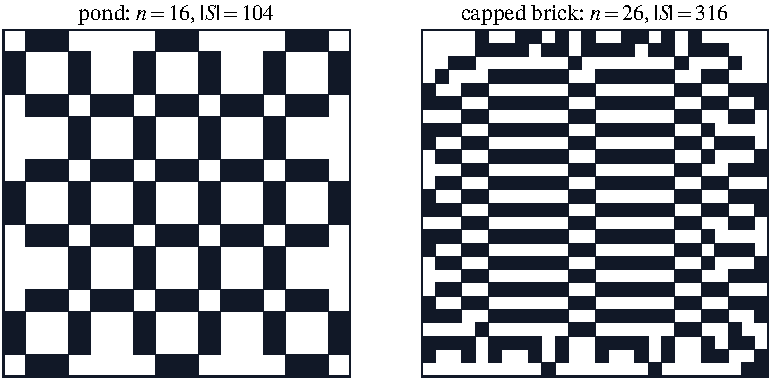
\includegraphics[width=.6\textwidth]{periodic_families.pdf}
\caption{Members of the pond and capped-brick families.}
\label{fig:periodic-families}
\end{figure}

\section{Computational certificates and ancillary data}\label{app:certificates}

The public repository~\cite{repo} contains the verified boards for
$2\le n\le50$, the boundary, equality-support, closure, and row certificates, two
independent board verifiers, regeneration scripts, regression tests, and a proof
index recording the upper-bound route for each exact value of its ledger.  The
certificates for the small proof-logged exclusions are those distributed with the
first version of this paper.  The directory \nolinkurl{ancillary/} accompanying
this version contains what is new in it: the eleven boards that improve lower
endpoints at $n=26,29,35,37,40,41,43,45,46,47,49$ (closing $n=29,37,41,45,49$),
the boards at $n=53,55,57,65$, the nine band-family seeds, the updated ledger,
the script that regenerates the figures and tables, and a standalone audit script.

The construction verifiers recompute the Life rule and connectivity from the grid
and do not trust stored counts.  The SAT objects are threshold statements: a
satisfying assignment at the target would refute the bound, whereas a checked
refutation proves it.

Running \texttt{python3 ancillary/scripts/verify\_manuscript.py}, which uses only
the Python standard library, recomputes the population, stability on the full
dead ring, and connectivity of every board used here; rebuilds the ledger for
$2\le n\le50$; checks the statements about exact values, open intervals, and the
chains of \cref{sec:closures-U}; and certifies the nine band families as in the
proof of \cref{thm:bands}.  It reads the upper bounds of the repository ledger
and does not replay the boundary, row, or closure certificates, which are audited
by the repository's own scripts.  The unrestricted maxima $M(n)$ are cited, not
recomputed.  No proof-assistant formalization is claimed.

\section{Atlas of verified boards}\label{app:atlas}

The verified board for every $n$ from $2$ to $50$, and the optimal boards at
$n=53,57,65$.  Solid blue frames mark proved optima; dashed gray frames mark open
sizes, labelled with the current interval.

\medskip
\noindent
\begin{minipage}[t]{.235\textwidth}\centering
\includegraphics[width=.92\linewidth]{atlas/n02.pdf}\\[1pt]{\scriptsize $n=2$: $C(n)=4$}\end{minipage}%
\hfill%
\begin{minipage}[t]{.235\textwidth}\centering
\includegraphics[width=.92\linewidth]{atlas/n03.pdf}\\[1pt]{\scriptsize $n=3$: $C(n)=6$}\end{minipage}%
\hfill%
\begin{minipage}[t]{.235\textwidth}\centering
\includegraphics[width=.92\linewidth]{atlas/n04.pdf}\\[1pt]{\scriptsize $n=4$: $C(n)=8$}\end{minipage}%
\hfill%
\begin{minipage}[t]{.235\textwidth}\centering
\includegraphics[width=.92\linewidth]{atlas/n05.pdf}\\[1pt]{\scriptsize $n=5$: $C(n)=11$}\end{minipage}%
\par\medskip\noindent
\begin{minipage}[t]{.235\textwidth}\centering
\includegraphics[width=.92\linewidth]{atlas/n06.pdf}\\[1pt]{\scriptsize $n=6$: $C(n)=18$}\end{minipage}%
\hfill%
\begin{minipage}[t]{.235\textwidth}\centering
\includegraphics[width=.92\linewidth]{atlas/n07.pdf}\\[1pt]{\scriptsize $n=7$: $C(n)=28$}\end{minipage}%
\hfill%
\begin{minipage}[t]{.235\textwidth}\centering
\includegraphics[width=.92\linewidth]{atlas/n08.pdf}\\[1pt]{\scriptsize $n=8$: $C(n)=32$}\end{minipage}%
\hfill%
\begin{minipage}[t]{.235\textwidth}\centering
\includegraphics[width=.92\linewidth]{atlas/n09.pdf}\\[1pt]{\scriptsize $n=9$: $C(n)=43$}\end{minipage}%
\par\medskip\noindent
\begin{minipage}[t]{.235\textwidth}\centering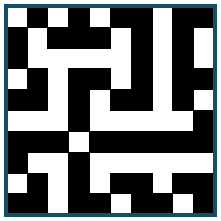
\includegraphics[width=.92\linewidth]{atlas/n10.pdf}\\[1pt]{\scriptsize $n=10$: $C(n)=53$}\end{minipage}%
\hfill%
\begin{minipage}[t]{.235\textwidth}\centering
\includegraphics[width=.92\linewidth]{atlas/n11.pdf}\\[1pt]{\scriptsize $n=11$: $C(n)=63$}\end{minipage}%
\hfill%
\begin{minipage}[t]{.235\textwidth}\centering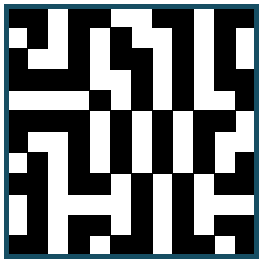
\includegraphics[width=.92\linewidth]{atlas/n12.pdf}\\[1pt]{\scriptsize $n=12$: $C(n)=76$}\end{minipage}%
\hfill%
\begin{minipage}[t]{.235\textwidth}\centering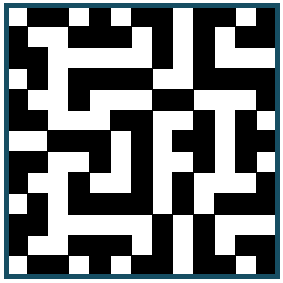
\includegraphics[width=.92\linewidth]{atlas/n13.pdf}\\[1pt]{\scriptsize $n=13$: $C(n)=88$}\end{minipage}%
\par\medskip\noindent
\begin{minipage}[t]{.235\textwidth}\centering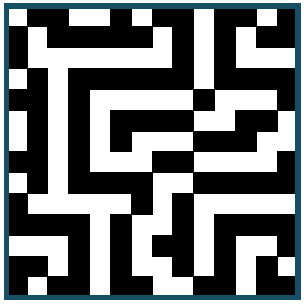
\includegraphics[width=.92\linewidth]{atlas/n14.pdf}\\[1pt]{\scriptsize $n=14$: $C(n)=102$}\end{minipage}%
\hfill%
\begin{minipage}[t]{.235\textwidth}\centering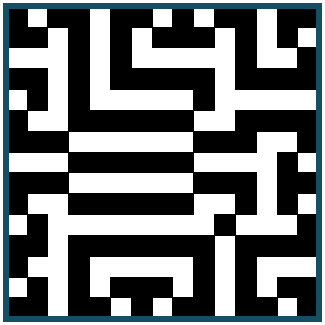
\includegraphics[width=.92\linewidth]{atlas/n15.pdf}\\[1pt]{\scriptsize $n=15$: $C(n)=119$}\end{minipage}%
\hfill%
\begin{minipage}[t]{.235\textwidth}\centering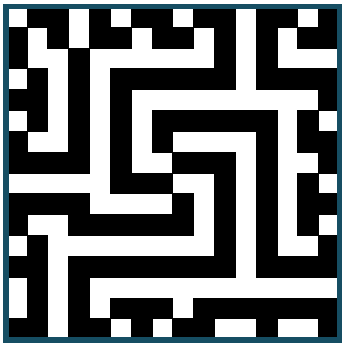
\includegraphics[width=.92\linewidth]{atlas/n16.pdf}\\[1pt]{\scriptsize $n=16$: $C(n)=134$}\end{minipage}%
\hfill%
\begin{minipage}[t]{.235\textwidth}\centering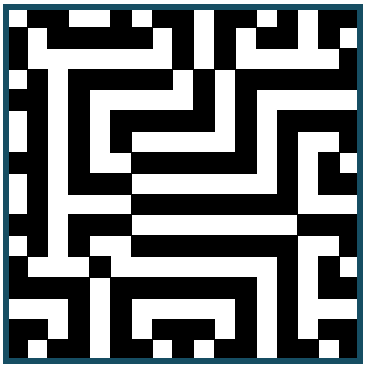
\includegraphics[width=.92\linewidth]{atlas/n17.pdf}\\[1pt]{\scriptsize $n=17$: $C(n)=151$}\end{minipage}%
\par\medskip\noindent
\begin{minipage}[t]{.235\textwidth}\centering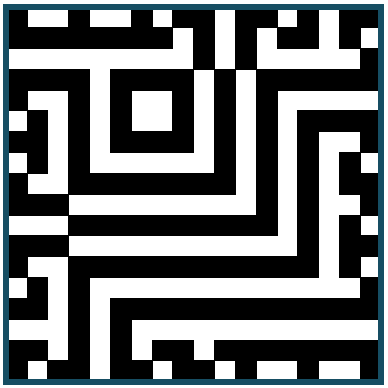
\includegraphics[width=.92\linewidth]{atlas/n18.pdf}\\[1pt]{\scriptsize $n=18$: $C(n)=170$}\end{minipage}%
\hfill%
\begin{minipage}[t]{.235\textwidth}\centering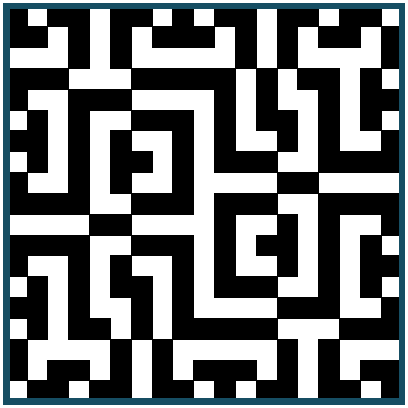
\includegraphics[width=.92\linewidth]{atlas/n19.pdf}\\[1pt]{\scriptsize $n=19$: $C(n)=188$}\end{minipage}%
\hfill%
\begin{minipage}[t]{.235\textwidth}\centering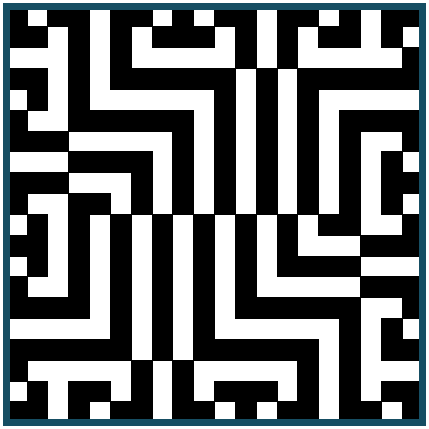
\includegraphics[width=.92\linewidth]{atlas/n20.pdf}\\[1pt]{\scriptsize $n=20$: $C(n)=210$}\end{minipage}%
\hfill%
\begin{minipage}[t]{.235\textwidth}\centering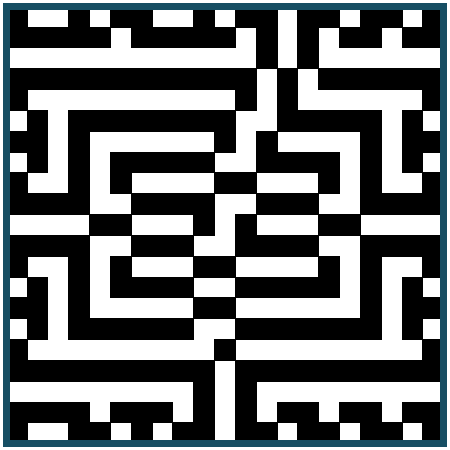
\includegraphics[width=.92\linewidth]{atlas/n21.pdf}\\[1pt]{\scriptsize $n=21$: $C(n)=230$}\end{minipage}%
\par\medskip\noindent
\begin{minipage}[t]{.235\textwidth}\centering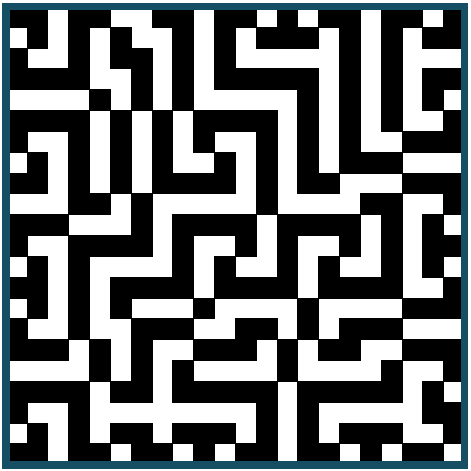
\includegraphics[width=.92\linewidth]{atlas/n22.pdf}\\[1pt]{\scriptsize $n=22$: $C(n)=251$}\end{minipage}%
\hfill%
\begin{minipage}[t]{.235\textwidth}\centering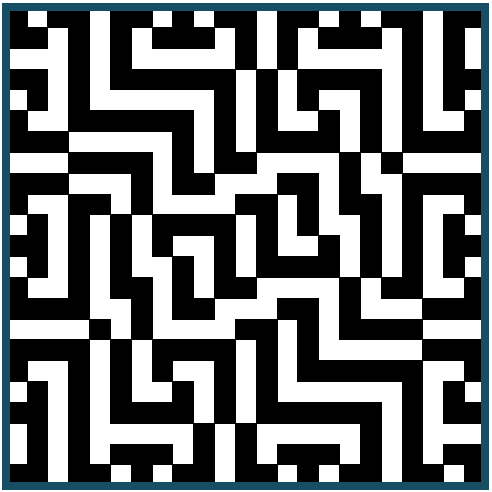
\includegraphics[width=.92\linewidth]{atlas/n23.pdf}\\[1pt]{\scriptsize $n=23$: $C(n)=276$}\end{minipage}%
\hfill%
\begin{minipage}[t]{.235\textwidth}\centering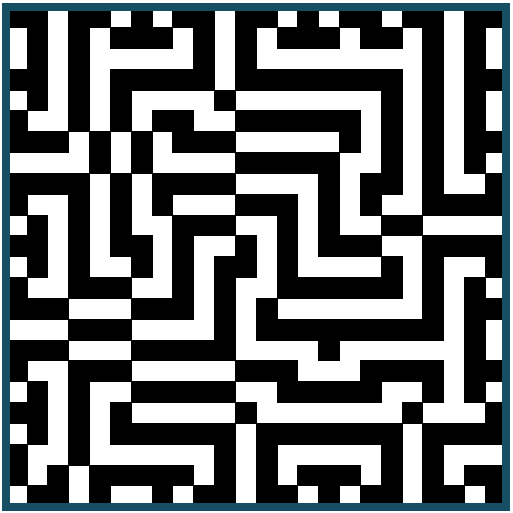
\includegraphics[width=.92\linewidth]{atlas/n24.pdf}\\[1pt]{\scriptsize $n=24$: $C(n)=299$}\end{minipage}%
\hfill%
\begin{minipage}[t]{.235\textwidth}\centering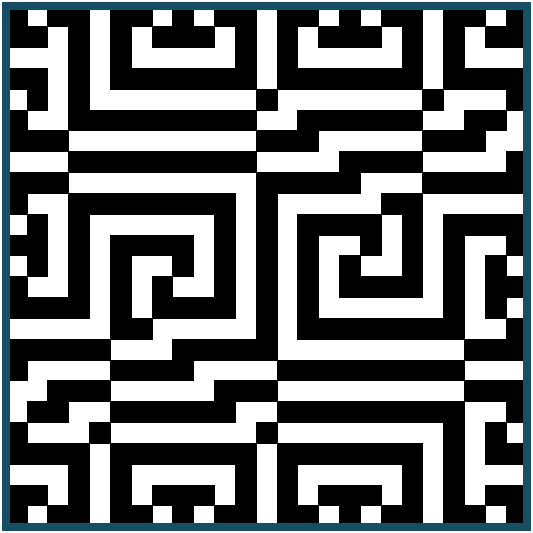
\includegraphics[width=.92\linewidth]{atlas/n25.pdf}\\[1pt]{\scriptsize $n=25$: $C(n)=325$}\end{minipage}%
\par\medskip\noindent
\begin{minipage}[t]{.235\textwidth}\centering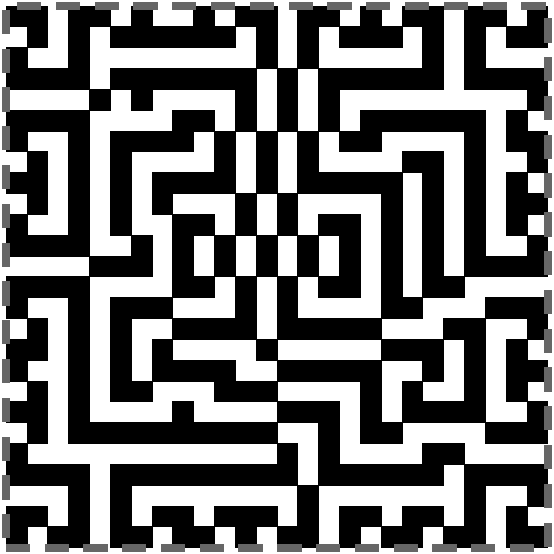
\includegraphics[width=.92\linewidth]{atlas/n26.pdf}\\[1pt]{\scriptsize $n=26$: $350\le C(n)\le352$}\end{minipage}%
\hfill%
\begin{minipage}[t]{.235\textwidth}\centering
\includegraphics[width=.92\linewidth]{atlas/n27.pdf}\\[1pt]{\scriptsize $n=27$: $375\le C(n)\le378$}\end{minipage}%
\hfill%
\begin{minipage}[t]{.235\textwidth}\centering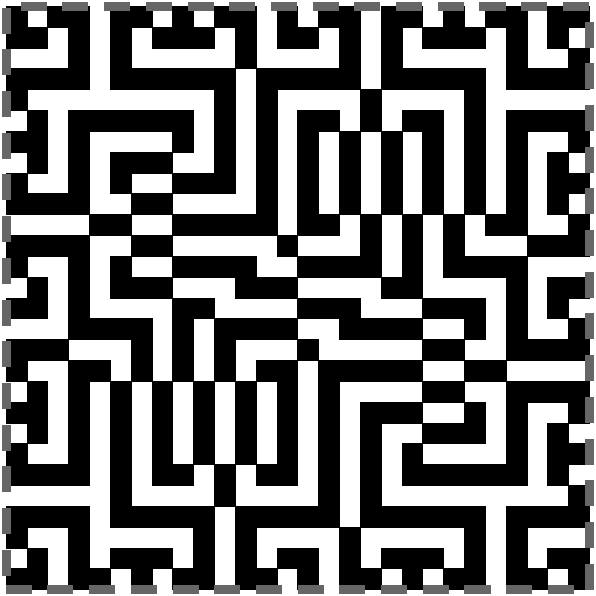
\includegraphics[width=.92\linewidth]{atlas/n28.pdf}\\[1pt]{\scriptsize $n=28$: $406\le C(n)\le407$}\end{minipage}%
\hfill%
\begin{minipage}[t]{.235\textwidth}\centering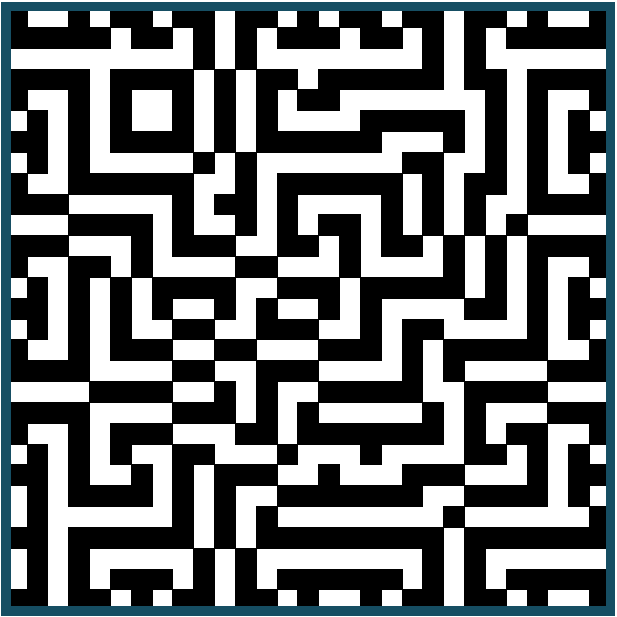
\includegraphics[width=.92\linewidth]{atlas/n29.pdf}\\[1pt]{\scriptsize $n=29$: $C(n)=435$}\end{minipage}%
\par\medskip\noindent
\begin{minipage}[t]{.235\textwidth}\centering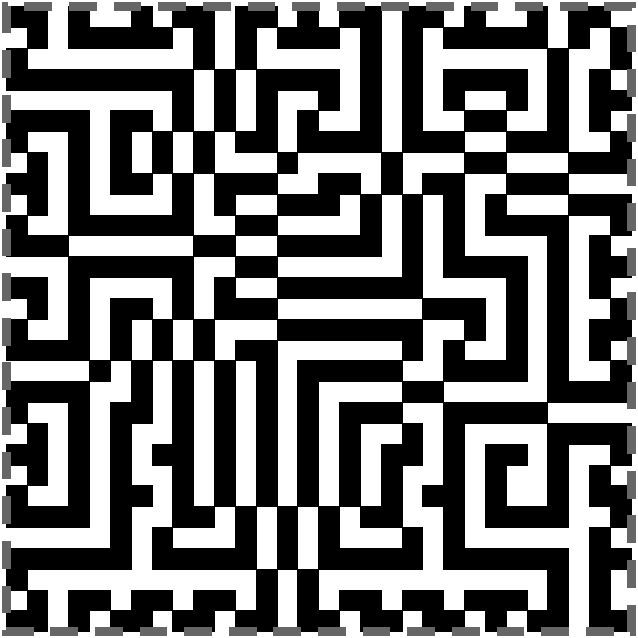
\includegraphics[width=.92\linewidth]{atlas/n30.pdf}\\[1pt]{\scriptsize $n=30$: $462\le C(n)\le465$}\end{minipage}%
\hfill%
\begin{minipage}[t]{.235\textwidth}\centering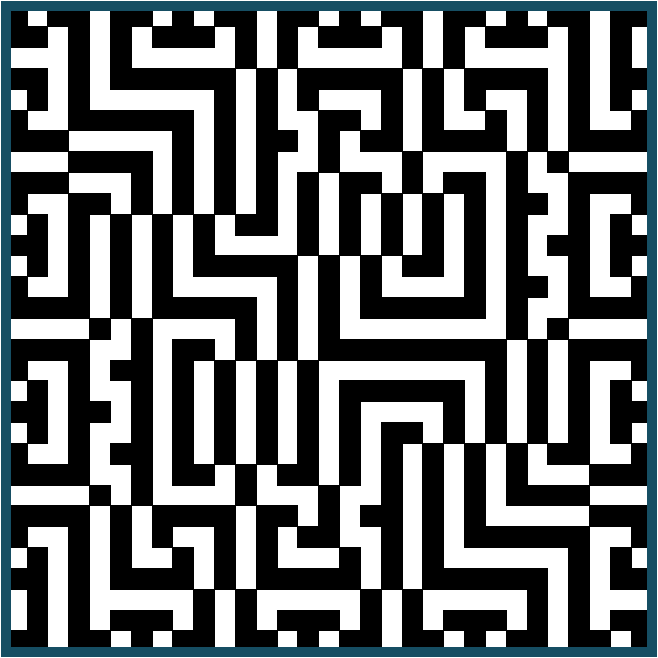
\includegraphics[width=.92\linewidth]{atlas/n31.pdf}\\[1pt]{\scriptsize $n=31$: $C(n)=497$}\end{minipage}%
\hfill%
\begin{minipage}[t]{.235\textwidth}\centering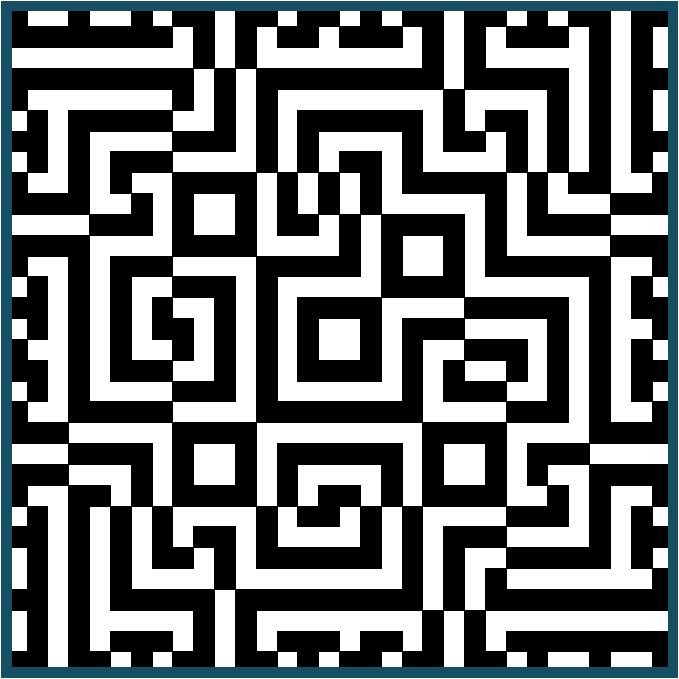
\includegraphics[width=.92\linewidth]{atlas/n32.pdf}\\[1pt]{\scriptsize $n=32$: $C(n)=528$}\end{minipage}%
\hfill%
\begin{minipage}[t]{.235\textwidth}\centering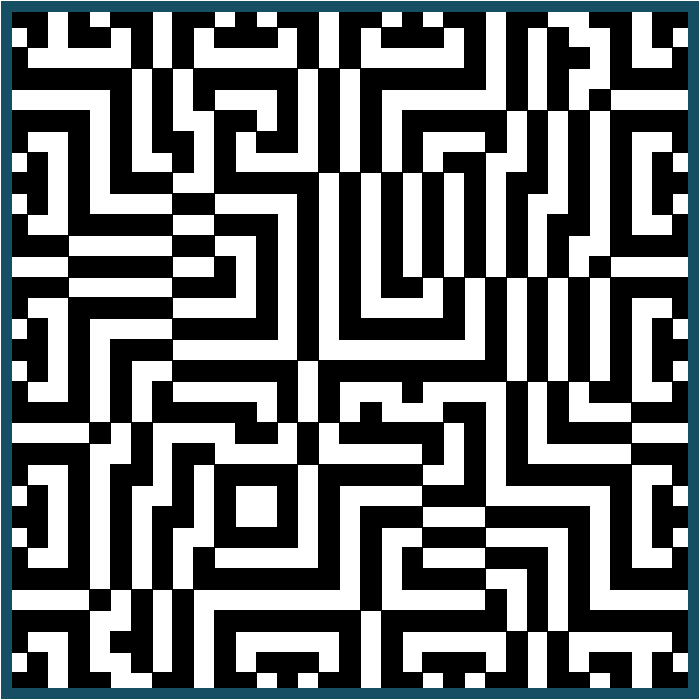
\includegraphics[width=.92\linewidth]{atlas/n33.pdf}\\[1pt]{\scriptsize $n=33$: $C(n)=562$}\end{minipage}%
\par\medskip\noindent
\begin{minipage}[t]{.235\textwidth}\centering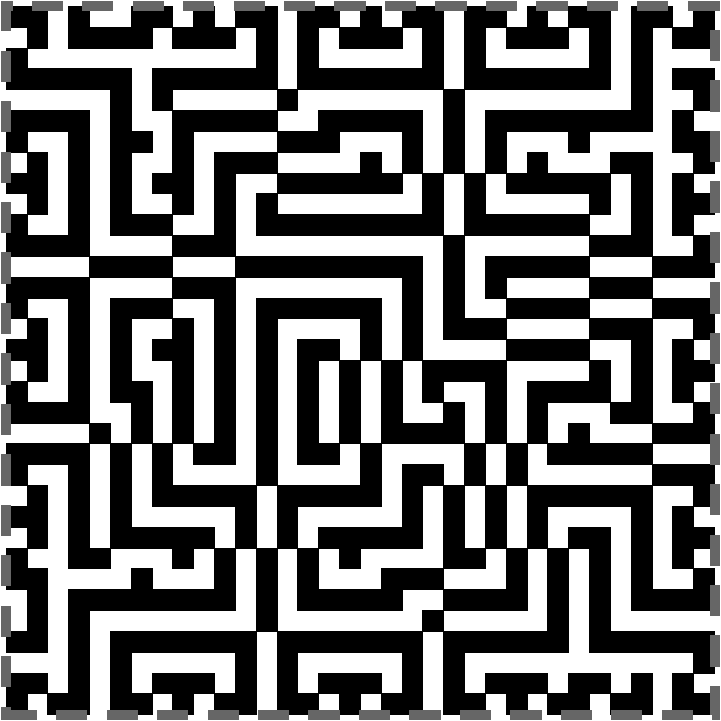
\includegraphics[width=.92\linewidth]{atlas/n34.pdf}\\[1pt]{\scriptsize $n=34$: $594\le C(n)\le597$}\end{minipage}%
\hfill%
\begin{minipage}[t]{.235\textwidth}\centering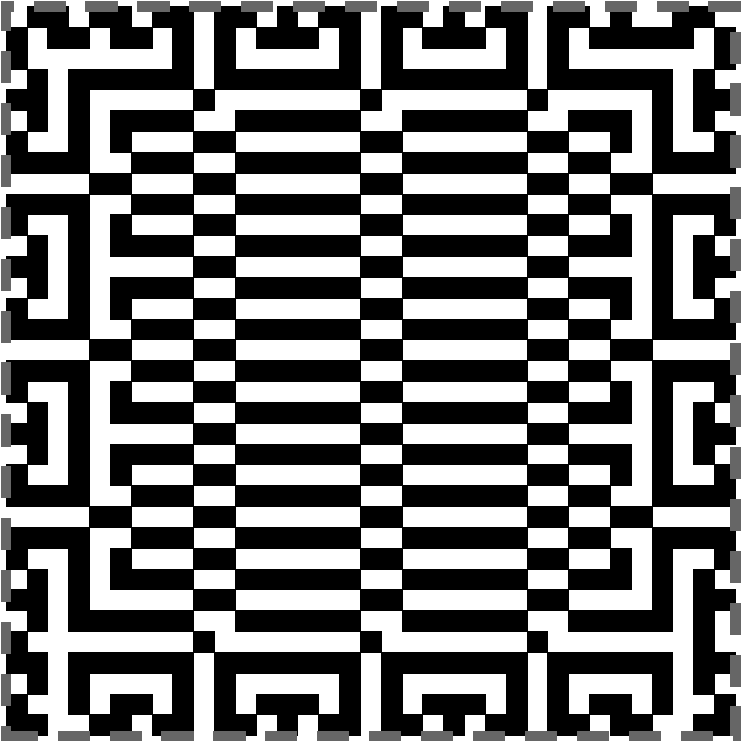
\includegraphics[width=.92\linewidth]{atlas/n35.pdf}\\[1pt]{\scriptsize $n=35$: $627\le C(n)\le631$}\end{minipage}%
\hfill%
\begin{minipage}[t]{.235\textwidth}\centering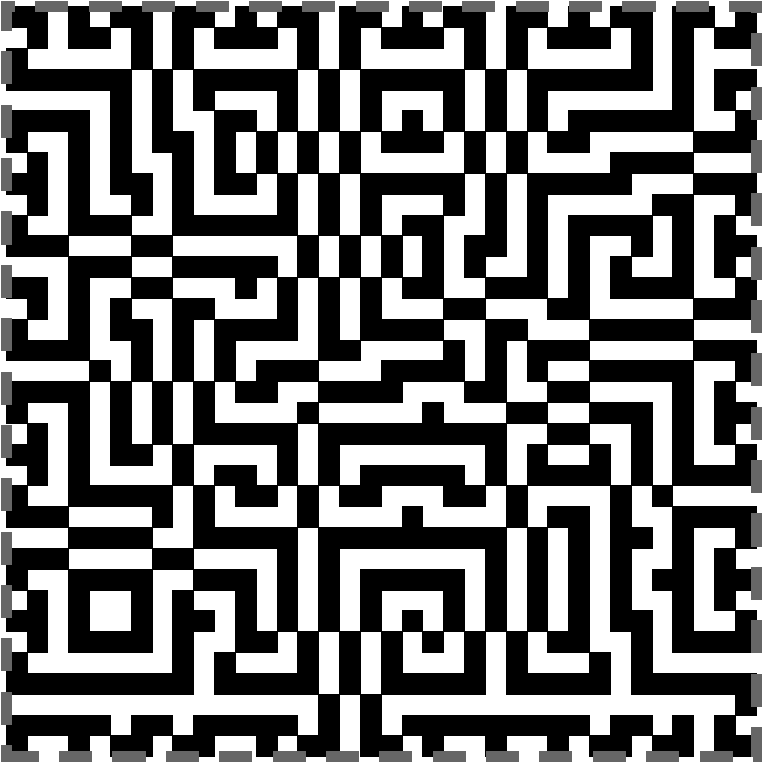
\includegraphics[width=.92\linewidth]{atlas/n36.pdf}\\[1pt]{\scriptsize $n=36$: $665\le C(n)\le668$}\end{minipage}%
\hfill%
\begin{minipage}[t]{.235\textwidth}\centering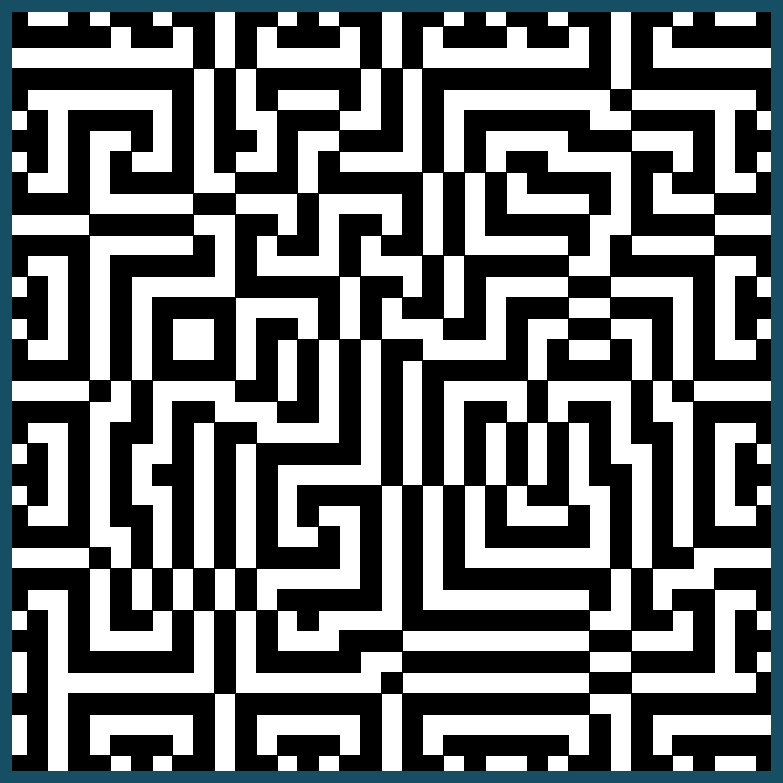
\includegraphics[width=.92\linewidth]{atlas/n37.pdf}\\[1pt]{\scriptsize $n=37$: $C(n)=704$}\end{minipage}%
\par\medskip\noindent
\begin{minipage}[t]{.235\textwidth}\centering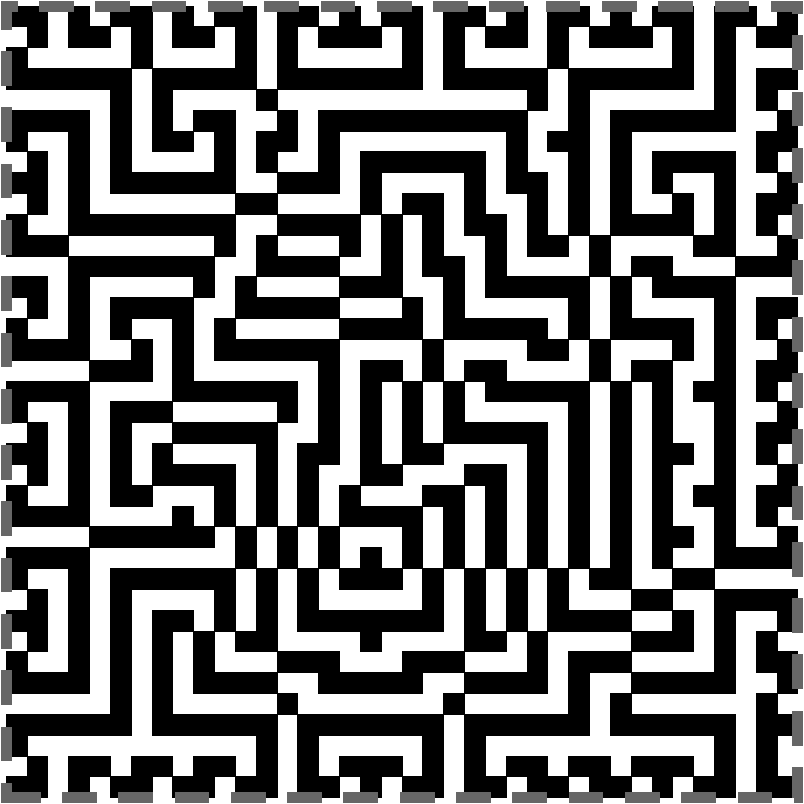
\includegraphics[width=.92\linewidth]{atlas/n38.pdf}\\[1pt]{\scriptsize $n=38$: $738\le C(n)\le742$}\end{minipage}%
\hfill%
\begin{minipage}[t]{.235\textwidth}\centering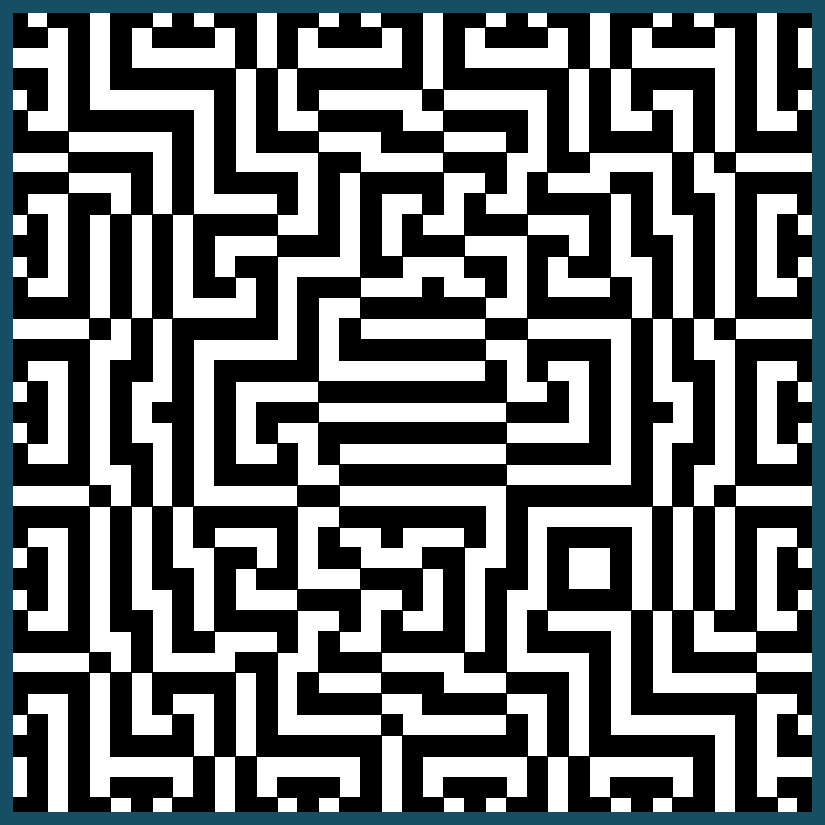
\includegraphics[width=.92\linewidth]{atlas/n39.pdf}\\[1pt]{\scriptsize $n=39$: $C(n)=782$}\end{minipage}%
\hfill%
\begin{minipage}[t]{.235\textwidth}\centering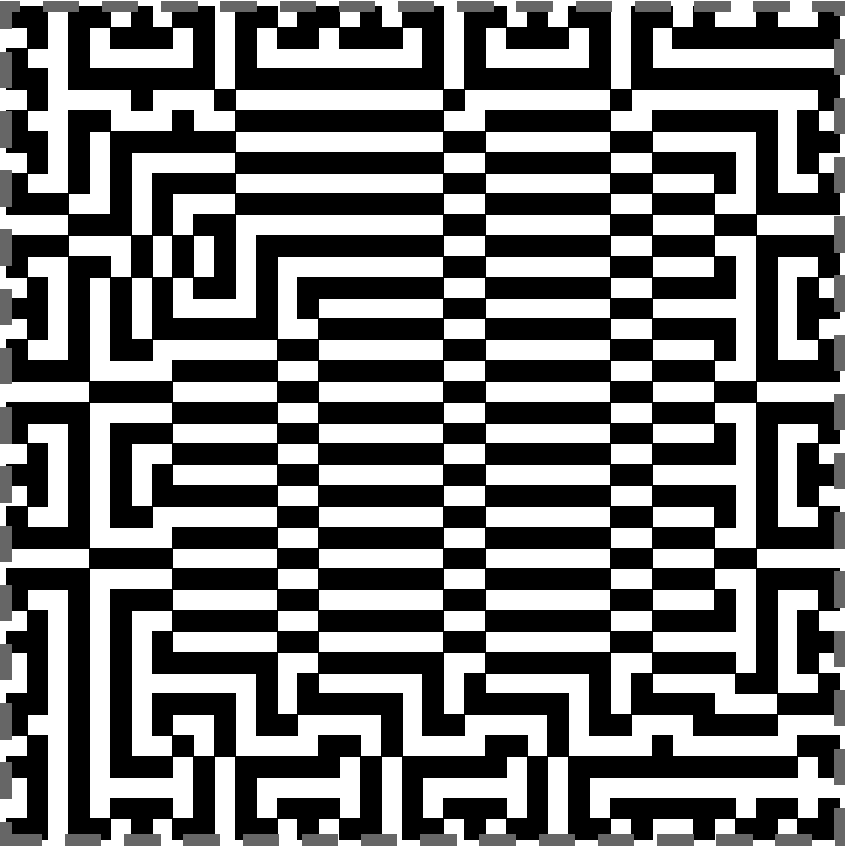
\includegraphics[width=.92\linewidth]{atlas/n40.pdf}\\[1pt]{\scriptsize $n=40$: $817\le C(n)\le821$}\end{minipage}%
\hfill%
\begin{minipage}[t]{.235\textwidth}\centering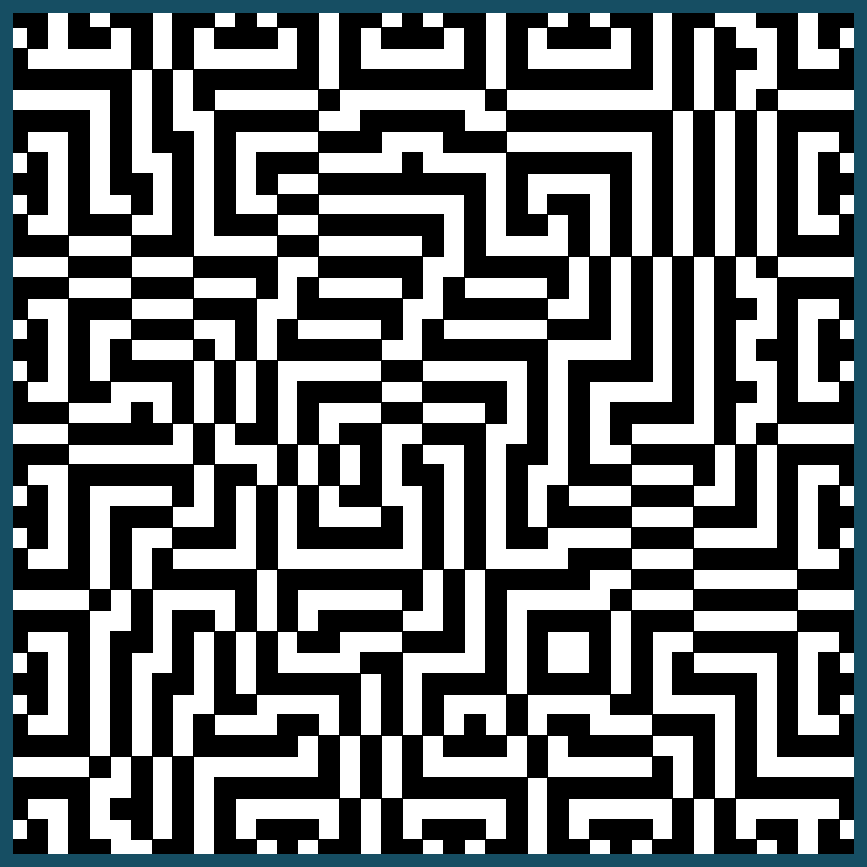
\includegraphics[width=.92\linewidth]{atlas/n41.pdf}\\[1pt]{\scriptsize $n=41$: $C(n)=863$}\end{minipage}%
\par\medskip\noindent
\begin{minipage}[t]{.235\textwidth}\centering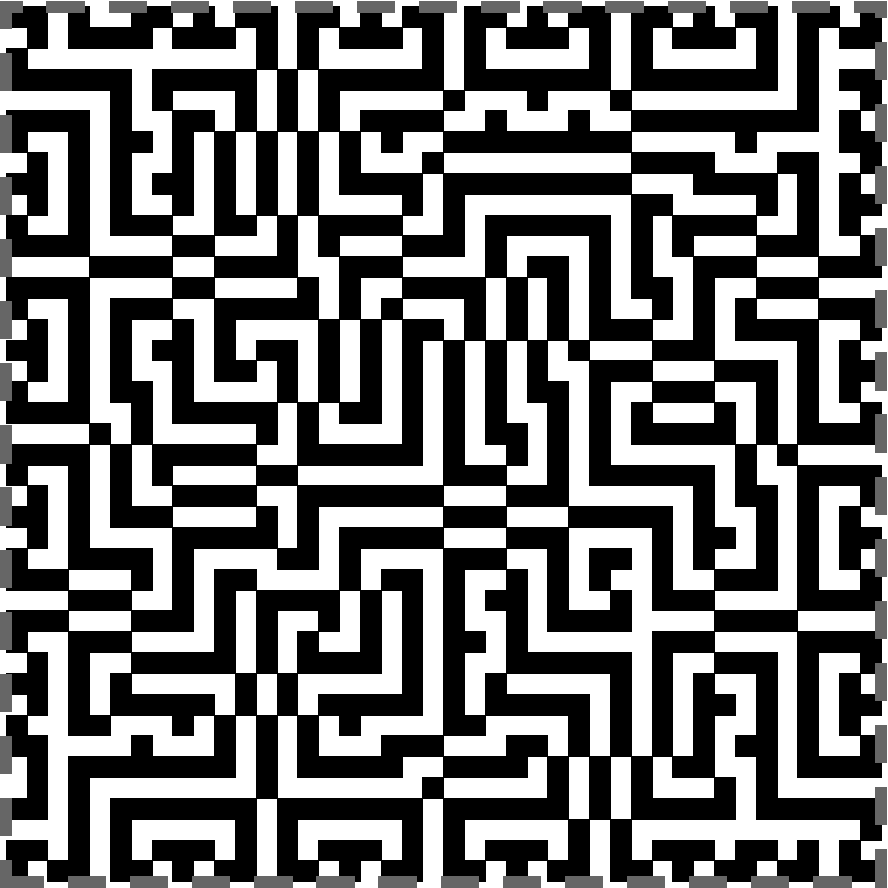
\includegraphics[width=.92\linewidth]{atlas/n42.pdf}\\[1pt]{\scriptsize $n=42$: $902\le C(n)\le906$}\end{minipage}%
\hfill%
\begin{minipage}[t]{.235\textwidth}\centering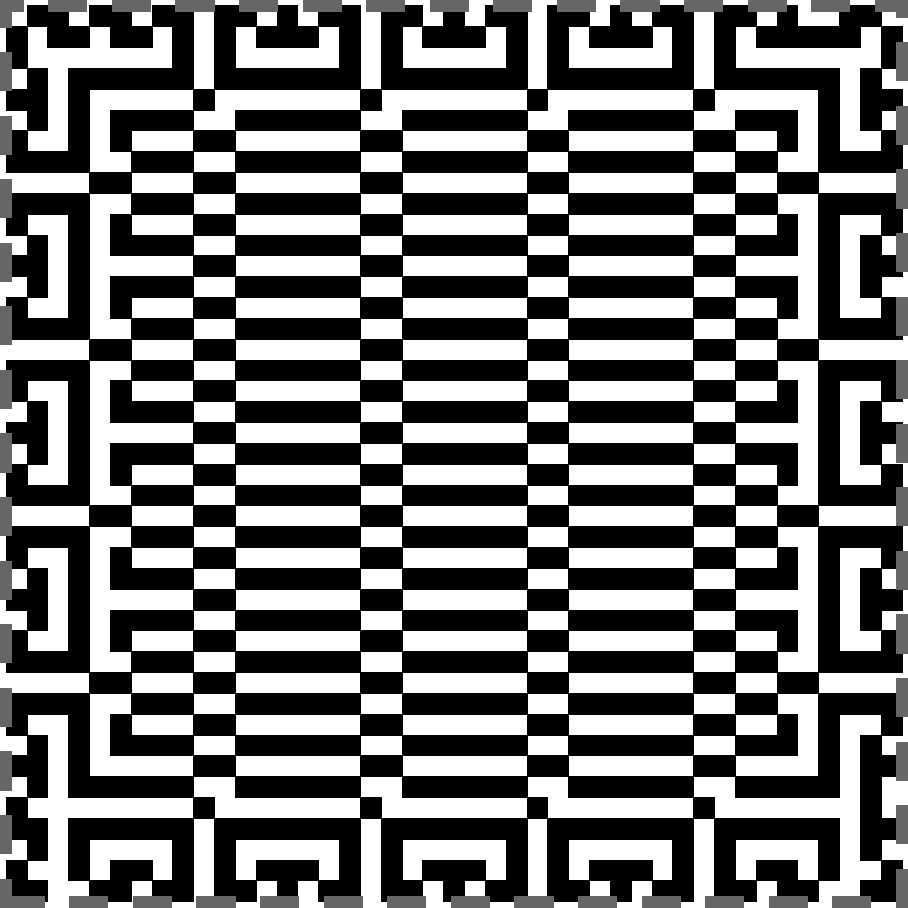
\includegraphics[width=.92\linewidth]{atlas/n43.pdf}\\[1pt]{\scriptsize $n=43$: $943\le C(n)\le948$}\end{minipage}%
\hfill%
\begin{minipage}[t]{.235\textwidth}\centering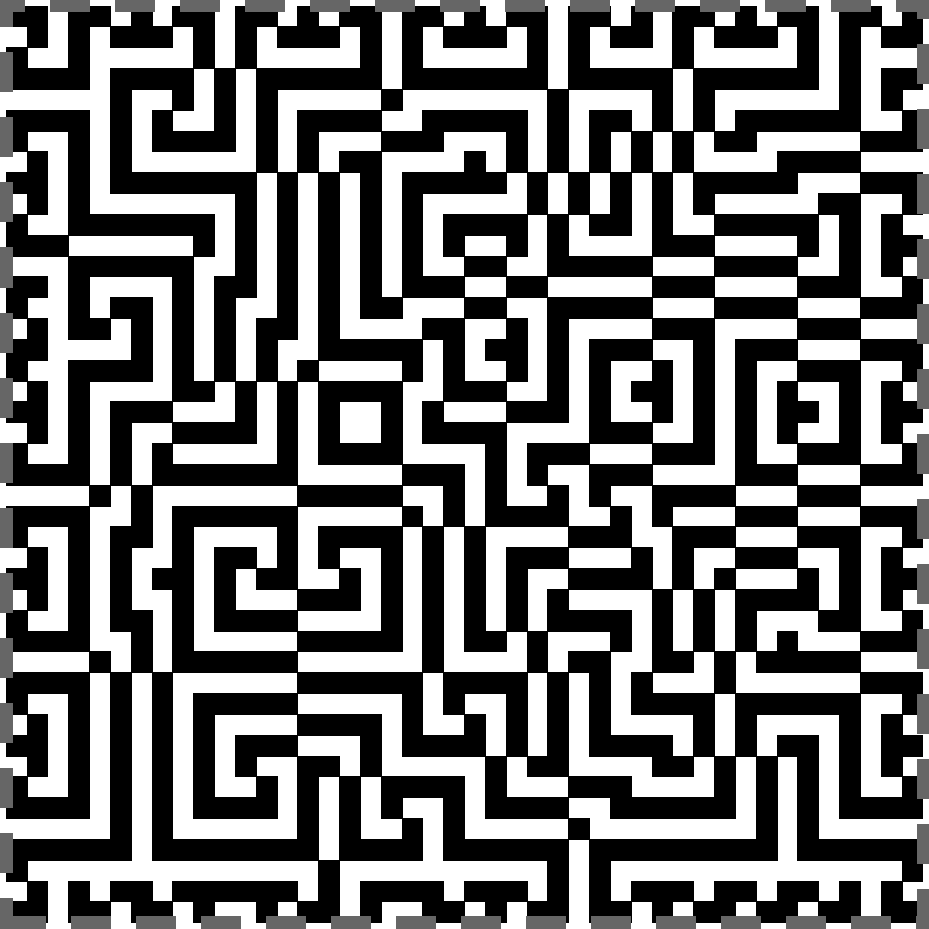
\includegraphics[width=.92\linewidth]{atlas/n44.pdf}\\[1pt]{\scriptsize $n=44$: $989\le C(n)\le993$}\end{minipage}%
\hfill%
\begin{minipage}[t]{.235\textwidth}\centering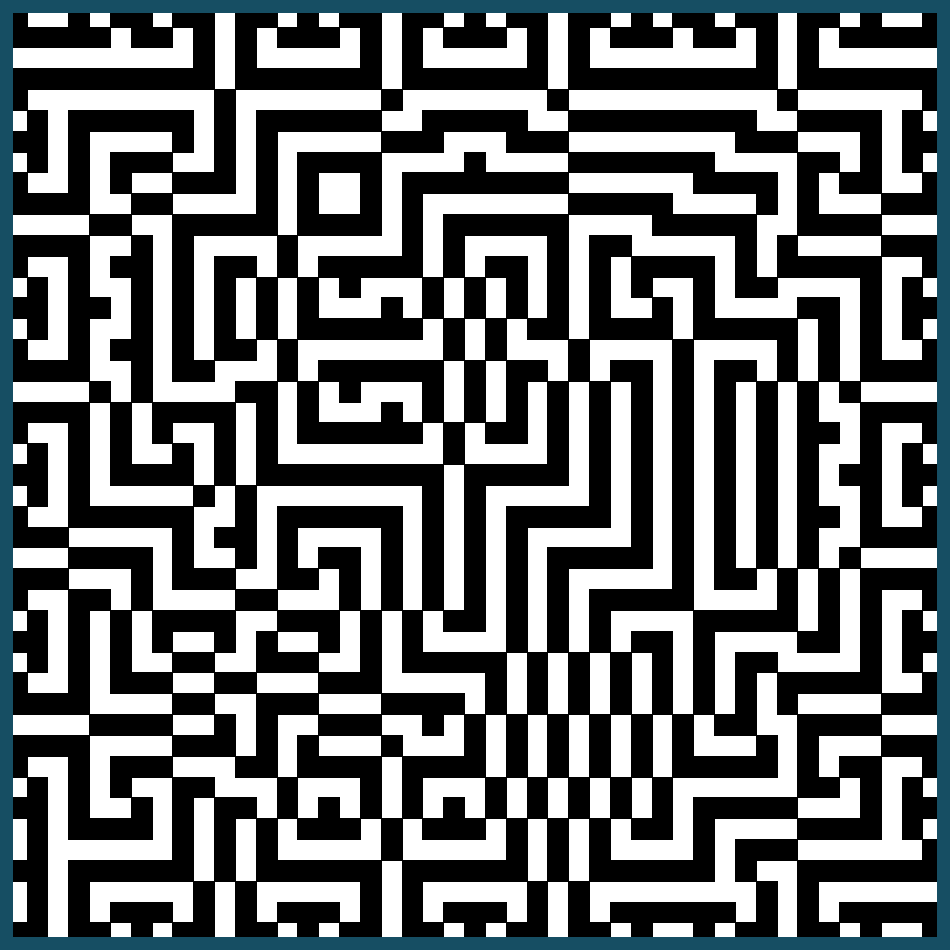
\includegraphics[width=.92\linewidth]{atlas/n45.pdf}\\[1pt]{\scriptsize $n=45$: $C(n)=1037$}\end{minipage}%
\par\medskip\noindent
\begin{minipage}[t]{.235\textwidth}\centering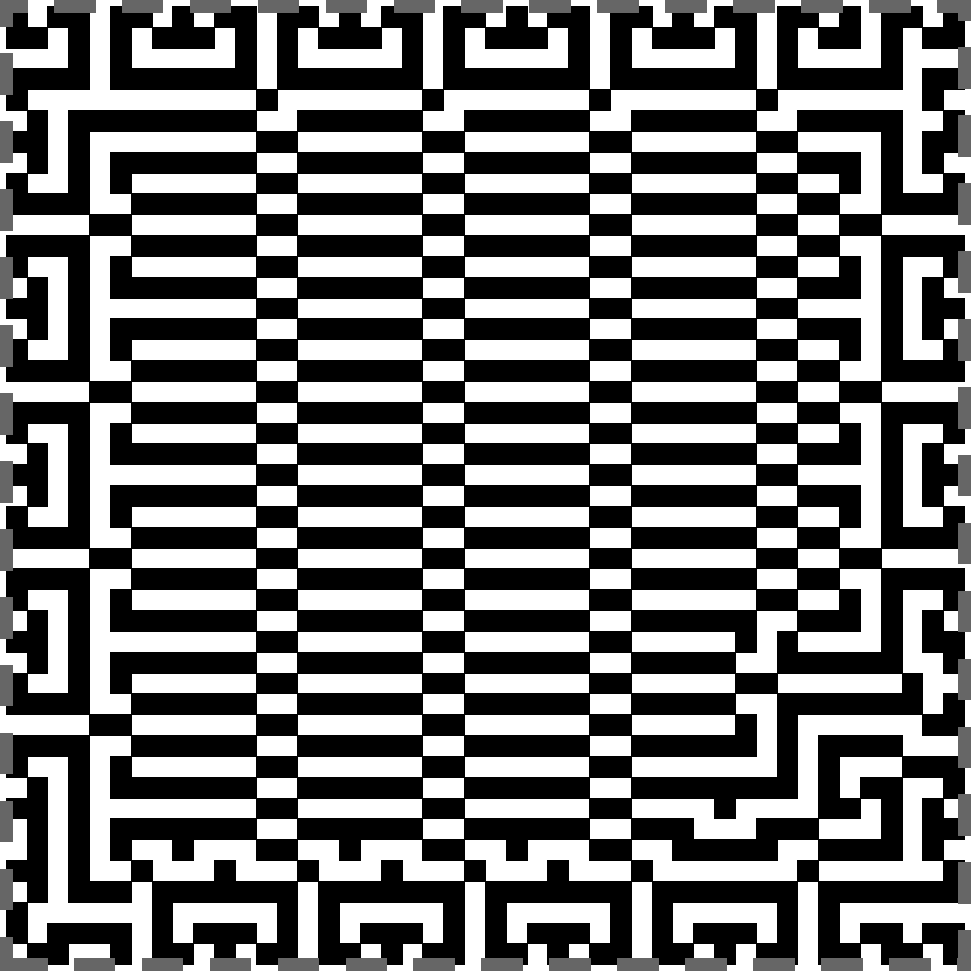
\includegraphics[width=.92\linewidth]{atlas/n46.pdf}\\[1pt]{\scriptsize $n=46$: $1078\le C(n)\le1083$}\end{minipage}%
\hfill%
\begin{minipage}[t]{.235\textwidth}\centering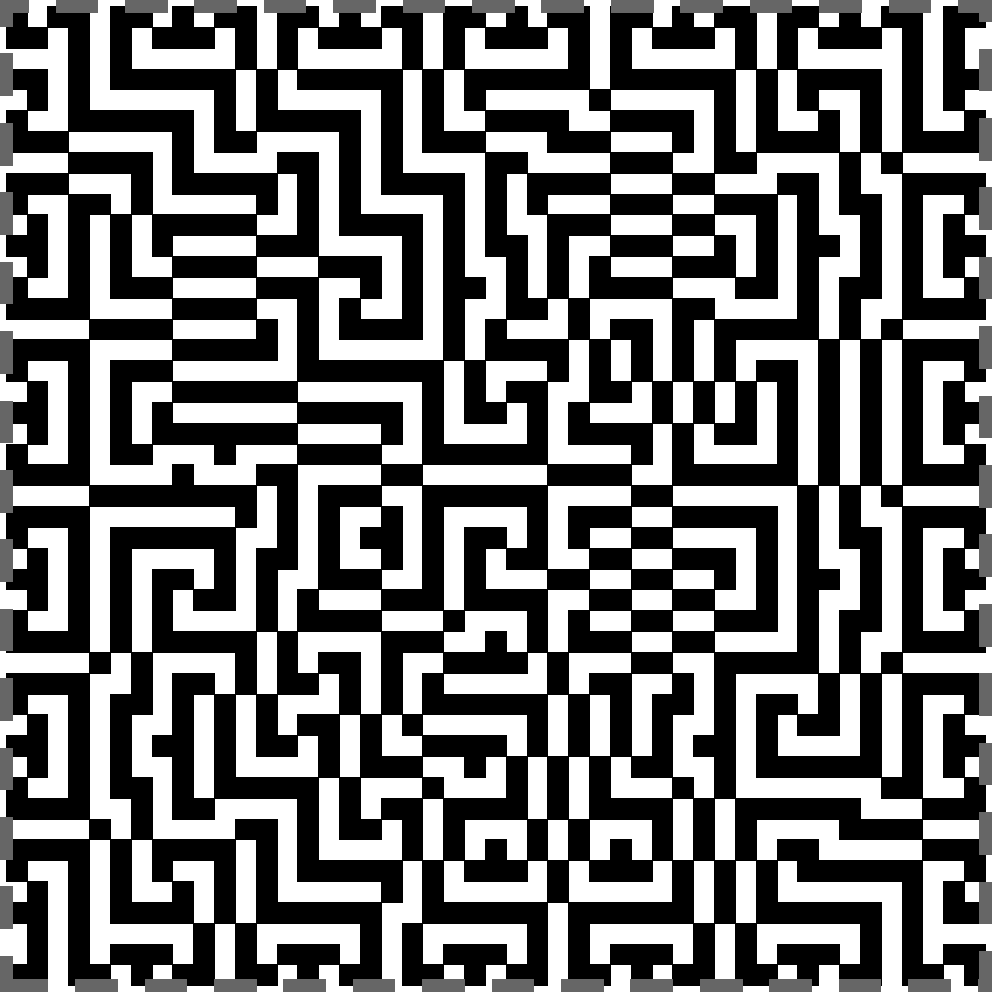
\includegraphics[width=.92\linewidth]{atlas/n47.pdf}\\[1pt]{\scriptsize $n=47$: $1131\le C(n)\le1132$}\end{minipage}%
\hfill%
\begin{minipage}[t]{.235\textwidth}\centering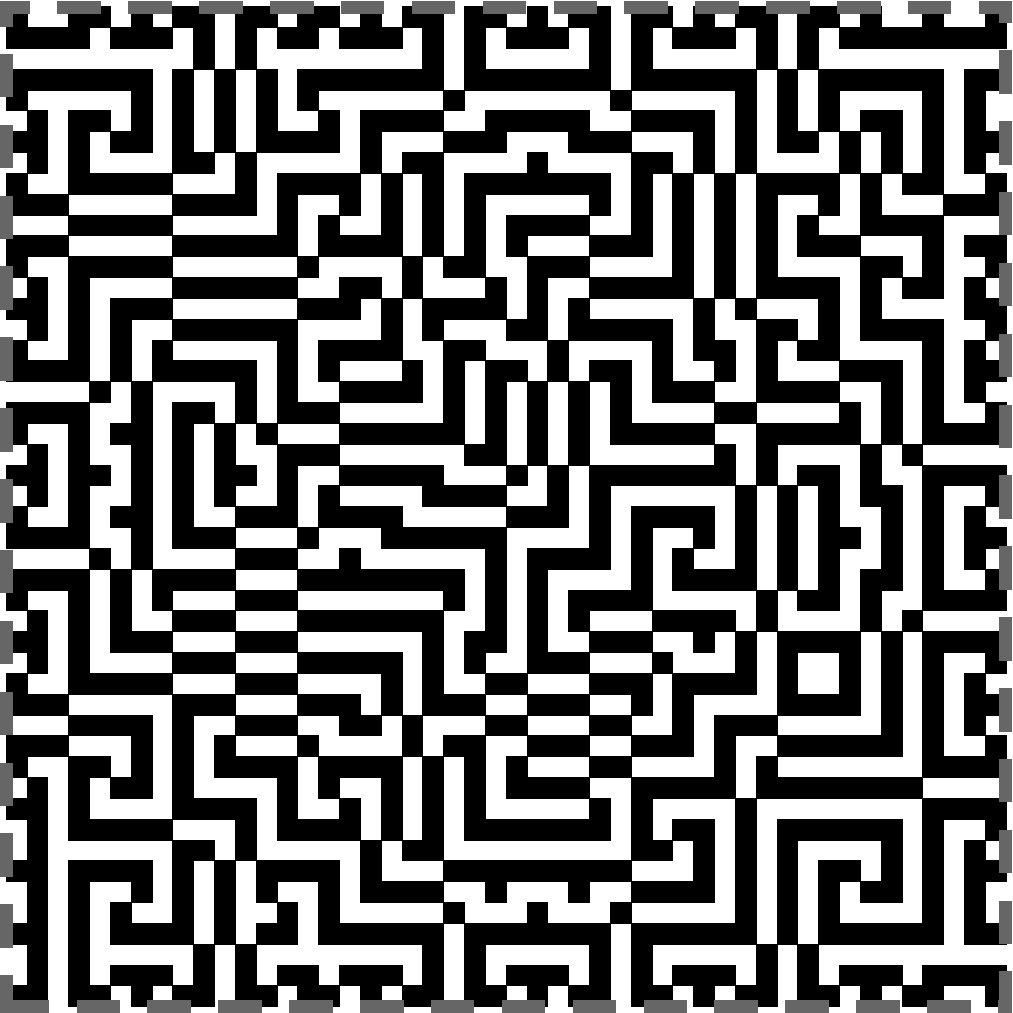
\includegraphics[width=.92\linewidth]{atlas/n48.pdf}\\[1pt]{\scriptsize $n=48$: $1174\le C(n)\le1178$}\end{minipage}%
\hfill%
\begin{minipage}[t]{.235\textwidth}\centering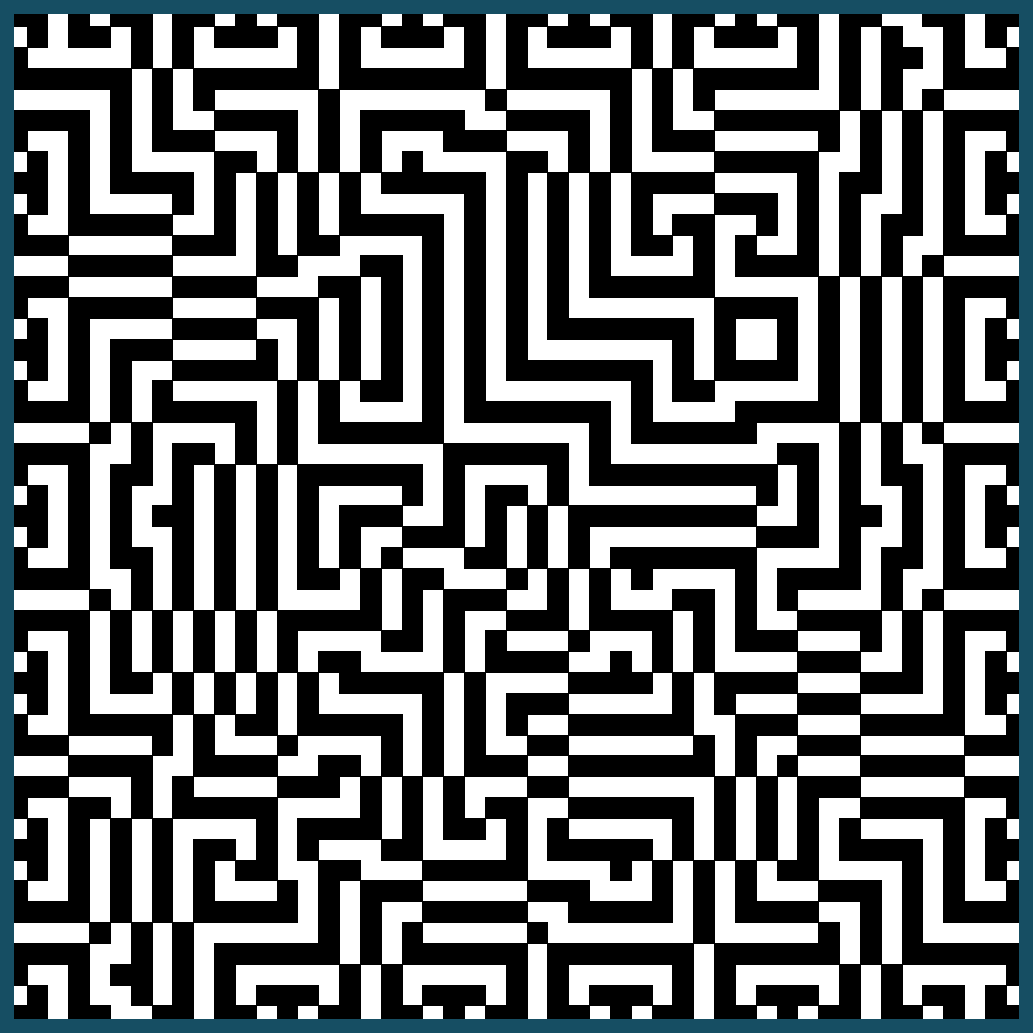
\includegraphics[width=.92\linewidth]{atlas/n49.pdf}\\[1pt]{\scriptsize $n=49$: $C(n)=1228$}\end{minipage}%
\par\medskip\noindent
\begin{minipage}[t]{.235\textwidth}\centering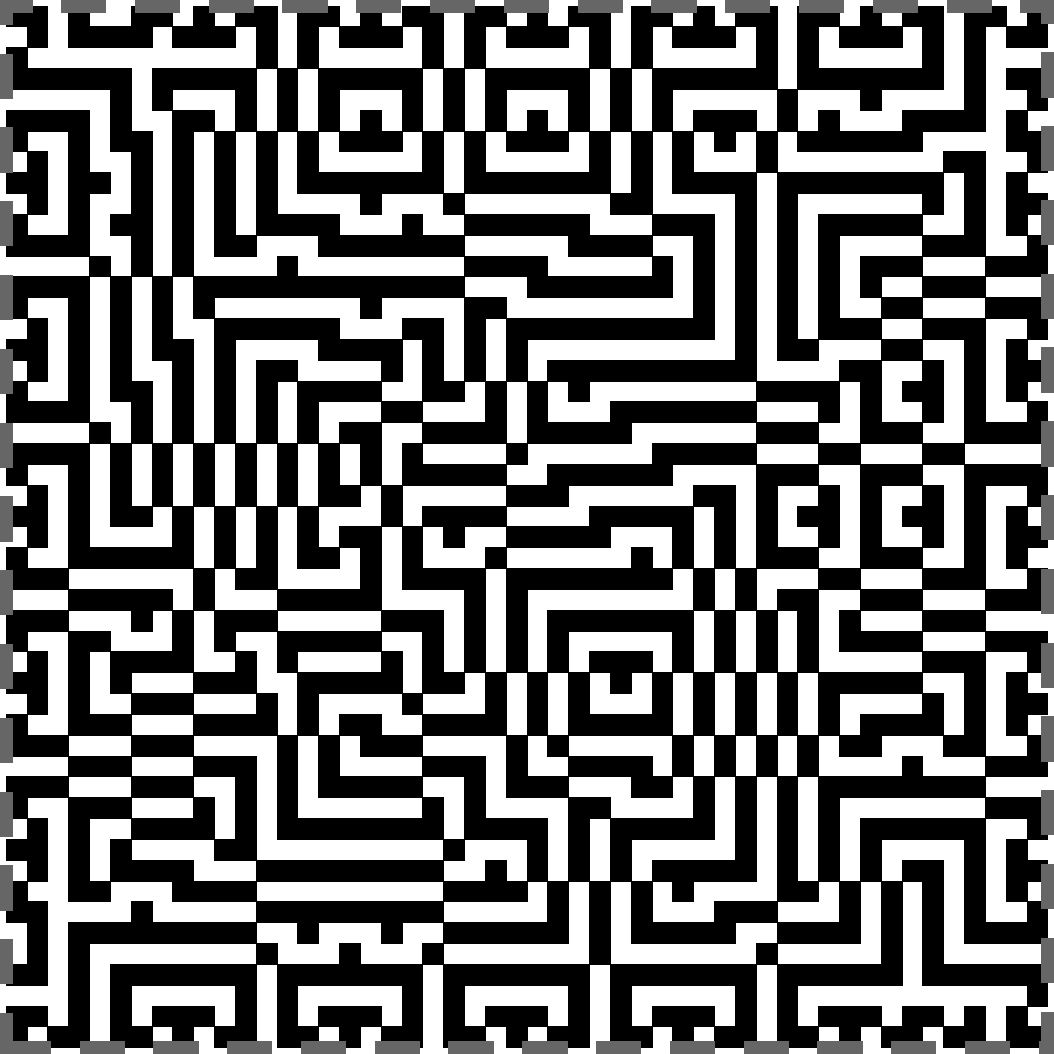
\includegraphics[width=.92\linewidth]{atlas/n50.pdf}\\[1pt]{\scriptsize $n=50$: $1276\le C(n)\le1279$}\end{minipage}%
\hfill%
\begin{minipage}[t]{.235\textwidth}\centering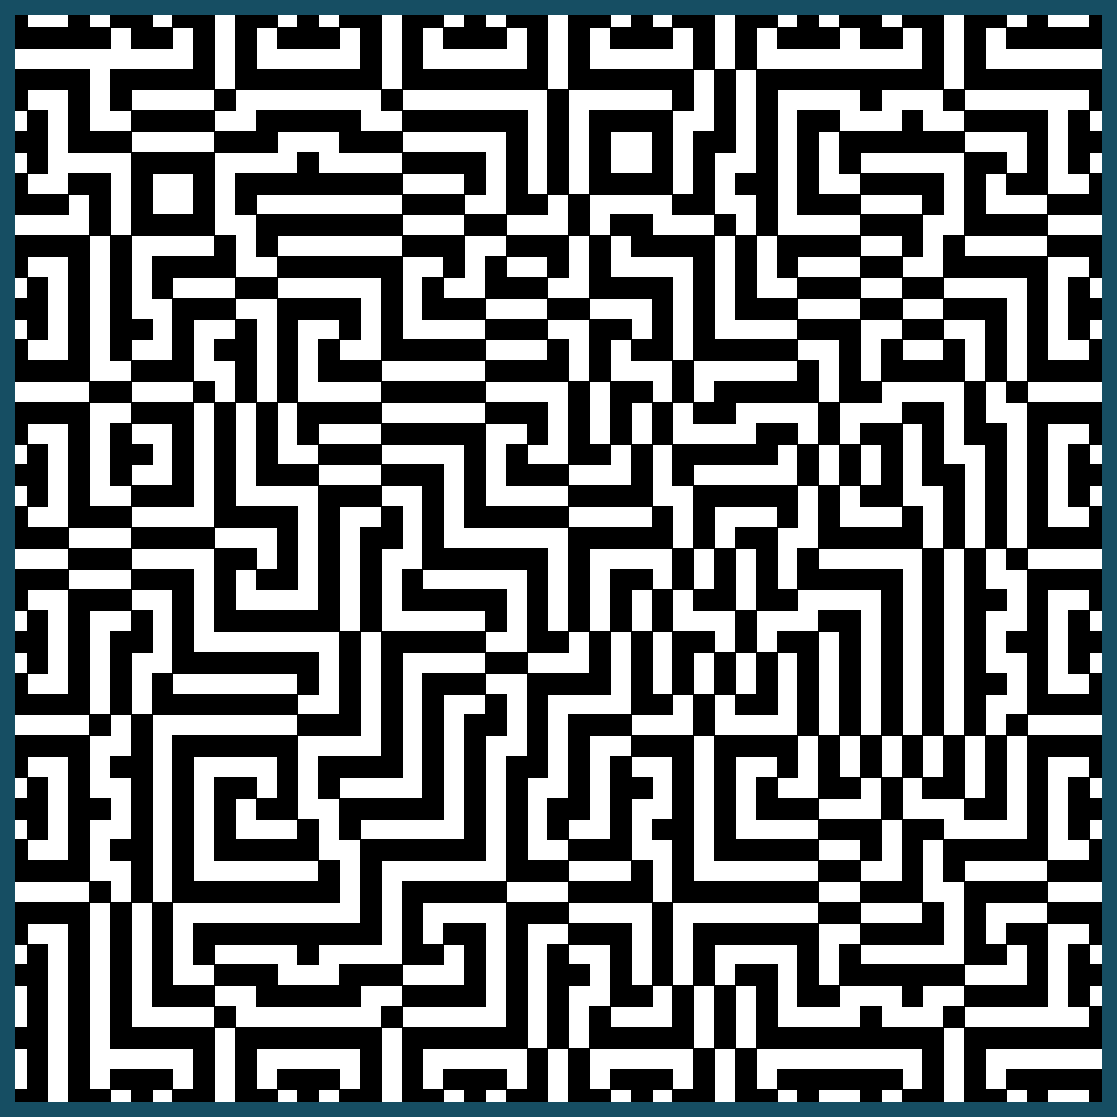
\includegraphics[width=.92\linewidth]{atlas/n53.pdf}\\[1pt]{\scriptsize $n=53$: $C(n)=1434$}\end{minipage}%
\hfill%
\begin{minipage}[t]{.235\textwidth}\centering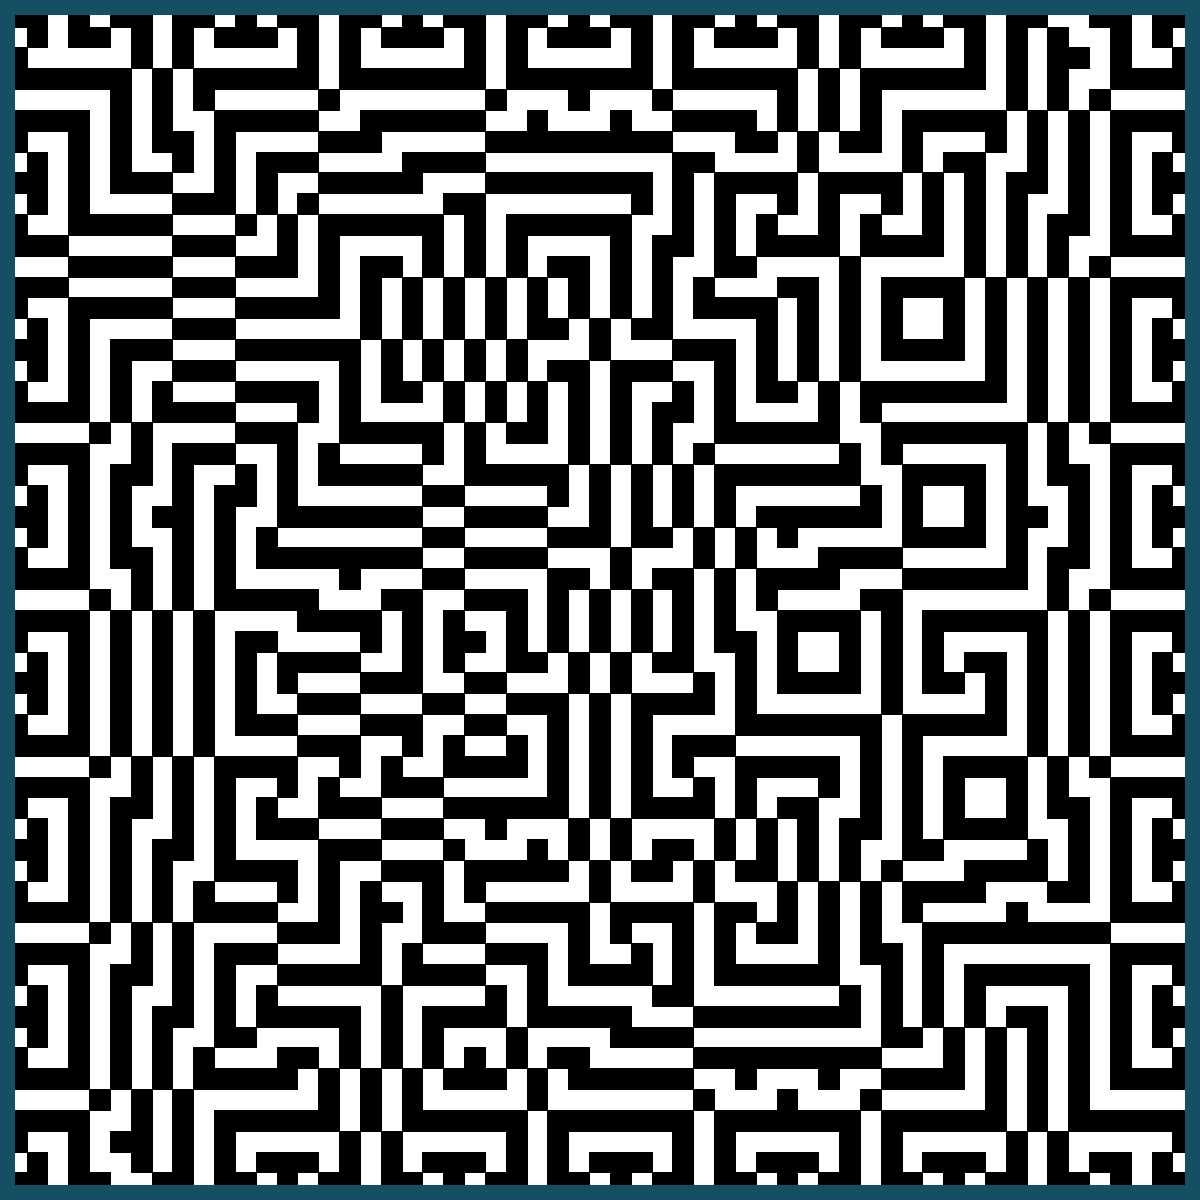
\includegraphics[width=.92\linewidth]{atlas/n57.pdf}\\[1pt]{\scriptsize $n=57$: $C(n)=1657$}\end{minipage}%
\hfill%
\begin{minipage}[t]{.235\textwidth}\centering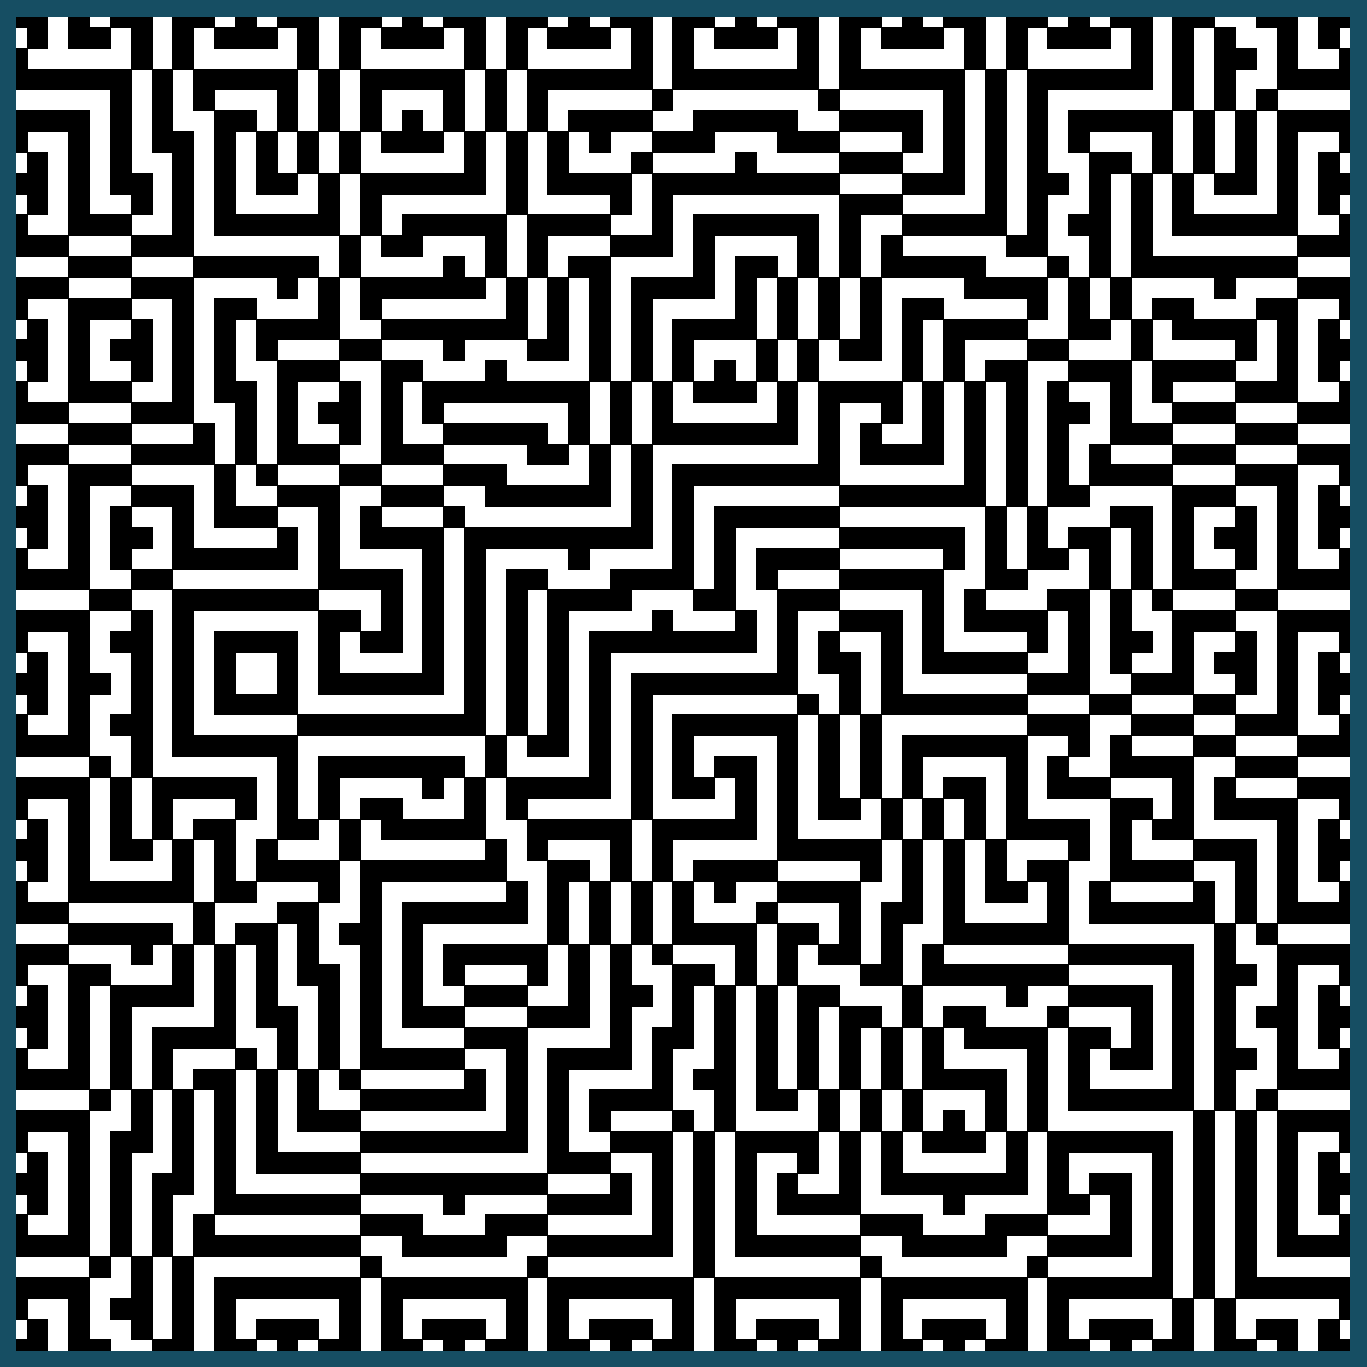
\includegraphics[width=.92\linewidth]{atlas/n65.pdf}\\[1pt]{\scriptsize $n=65$: $C(n)=2150$}\end{minipage}%
\par\medskip\noindent


\end{document}
